\title{DISCRETE GROUPS AND Q-STRUCTURES ON SEMI-SIMPLE LIE GROUPS}
\markright{DISCRETE GROUPS AND Q-STRUCTURES ON SEMI-SIMPLE LIE GROUPS}

\author{By~ M. S. RAGHUNATHAN}
\markboth{M. S. RAGHUNATHAN}{DISCRETE GROUPS AND Q-STRUCTURES ON SEMI-SIMPLE LIE GROUPS}

\date{}
\maketitle


%\setcounter{page}{21}
\setcounter{pageoriginal}{224}

\noindent
\textsc{Introduction.} The\pageoriginale main aim of this paper is to establish the following result.

\begin{maintheorem*}
Let $G$ be a connected linear semisimple algebraic group defined over $\bR$ of $\bR$-rank $\geqslant$ 2 and with trivial centre. Let $G$ be the connected component of the identity in $\bG_{\bR}$, the group of $\bR$-rational points of $\bG$. Assume that $G$ has no non-trivial compact connected normal subgroup. Let $\Gamma \subset G$ be a discrete subgroup such that $G/\Gamma$ is non-compact ans has finite Haar measure. Assume further that $\Gamma \cap G'$ is finite for every connected proper normal subgroup $G'$ of $G$. Then there exists a $\bQ$-algebraic group $\bG^\ast$ and an isomorphism (defined over $\bR$)  $f: \bG^\ast \to \bG$ such that $f^{-1} (\Gamma) \subset G^\ast_\bQ$ and for every proper $\bQ$-parabolic subgroup $\bP$ of $G^\ast$, $\bP \cap f^{-1} (\Gamma)$ is an arithmetic subgroup of $\bP$.

If in addition, there exists a unipotent $\theta \in \Gamma$ which is contained in two distinct maximal unipotent subgroups of $\theta \in \Gamma$ which is contained in two distinct maximal unipotent subgroups of $\Gamma$, then $f^{-1}(\Gamma)$ is an arithmetic subgroup of $\bG^\ast$; in this case, $\bQ$-rank $\bG^\ast \geqslant 2$.
\end{maintheorem*}

The main theorem with the exception of the last assertion was announced by Margolis \cite{art9-key1} in 1969. (In a recent letter Margolis informs the author that he has proved the arithmeticity of $f^{-1}(\Gamma)$ in all cases.) As no proofs were available for a long time the present author pursued the problem on his own despite the announcement. Most of the work in this paper was done while the author was visiting at Osaka University during March-June 1972. The author would like to take this opportunity to express his warmest thanks to the J.S.P.S. and Professor Murakami and his colleagues for their king hospitality. Later, in January 1973, the author spoke on the work at the International Colloquium on ``Discrete subgroups of Lie groups'' held in Bombay.\footnote{The proofs given here are somewhat different from those outlined in the talk.}

Margolis' proof is apparently based on the following result:

\begin{theorem*}
Let $X \in M(n, \bR)$\pageoriginale be a nilpotent matrix. Then the map $f: \bR \to SL (n, \bR)/ SL (n, \bZ)$ defined by $f(t) = \pi(\exp t X)$, where $\pi: SL (n, \bR) \to S L (n, \bR)/ SL (n,\bZ)$ is the natural map, is not proper.
\end{theorem*}

(A proof of the theorem by Margolis \cite{art9-key2} has appeared. The result was conjectured first by Pjatetski-Shapiro \cite{art9-key1} and some years later, independently by H. Garland and the author (see Raghunathan \cite{art9-key4})).

The author tried without success to prove this result and eventually obtained the main theorem without the use of the lemma. Some parts of this paper especially in \S \ref{art9-sec2} can perhaps be shortened with the aid of this theorem; but it does not help shorten the paper on the whole significantly. A theorem proved by the author (Raghunathan \cite{art9-key1}, Theorem 11.16) can in some ways be regarded as the starting point. Repeated use is also made of the basic result on the existence of unipotent elements in discrete groups due to Kazdan-Margolis \cite{art9-key1}.

We now indicate how the main result is proved explaining in the process also how the paper is organised.

The main result above is formulated for lattices. However, we will work with what we call ``$L$-subgroups''. The class of $L$-subgroups is \textit{a priori} a wider class than that of lattices. (However, at the end of the paper one finds that $L$-subgroups are indeed lattices). In \S \ref{art9-sec1} we generalise Borel's density theorem (Borel \cite{art9-key1}) to $L$-subgroups. A justification for including this material here can perhaps be found in the following: that arithmetic subgroups are $L$-subgroups is essentially the Godement compactness-criterion which is only the first step towards proving that arithmetic groups are indeed lattices.\footnote{Curiously enough, we never use the fact, that arithmetic groups are lattices, in this paper.} The impatient reader can skip this section beyond \S \ref{art9-subsec1.8} altogether and go on to \S \ref{art9-sec2}. He need only read ``lattice'' for ``$L$-subgroup'' everywhere.

The material in \S \ref{art9-sec2} contains the most difficult steps.  We prove here the following (notation as in the statement of the main theorem):

There exists an $\bR$-parabolic subgroup $\bN$ of $\bG$ and a normal $\bR$-subgroup $\bN_0$ of codimension  1 in $\bN$ containing the unipotent radical\pageoriginale  $\bF$ of $\bN$ with the following properties: let $\bL$ be the Zariski-closure of $\bN \cap \Gamma$  in $\bG$ and $\bE$ the centre of $\bF$; then $\bL/\bE$ and $\bF$ carry natural $\bQ$-structures such that (a) $\bF \cap \Gamma$ (\resp. image of $\bL\cap \Gamma$ in $\bL/ \bE$)is arithmetic and (b) the natural action of $\bL/\bE$ on $\bF$ is defined over $\bQ$; moreover if $L = \bL \cap G$ and $N_0 = \bN_0 \cap G$, then $L \subset N_0$ and $N_0/ L$ is compact.

The proof is involved and rather difficult to outline. It makes use of the techniques---not merely the final results---of Kazdan and Margolis \cite{art9-key1}. In this section, we also introduce the notion of rank for an $L$-subgroup. $L$-subgroups of rank 1 and rank $> 1$ are treated separately in the subsequent sections.

\S\ref{art9-sec3} begins with the following characterisation of $L$-subgroups of rank 1. 

$\Gamma \subset G$ is ($L$-subgroup) of rank 1 if and only if every unipotent ($\neq$ identity) in $\Gamma$ is contained in a unique maximal unipotent subgroup of $\Gamma$.

The case of rank 1 $L$-subgroups is then handled as follows. One starts with a parabolic subgroup $\bN$ as described above and shows that a conjugate of $\bN$ by any element of $\Gamma$ not in $\bN$ is opposed to $\bN$; as a consequence one obtains a semi-direct product decomposition $\bN = \bM. \bF$ with $\bF$ the unipotent radical such that $(\bM \cap \Gamma) (\bF \cap \Gamma)$  has finite index in $\bN \cap \Gamma$. Also the assumption that $\bR$-rank $\bG>1$ guarantees that $\bM \cap \Gamma$ is sufficiently big (to guarantee that its centraliser in $\bF$ is in the centre of $\sF$). If $\bM_1$ is the Zariski-closure of $\bM \cap \Gamma$, then $\bD = \bM_1 \cdot \bF$ has a natural $\bQ$-structure in which $\bD \cap \Gamma$ is arithmetic. Now let $\theta \in \Gamma -N$; then $\bM^\theta_1 = \theta \bN \theta^{-1} \cap \bD$ is shown to be a maximal reductive $\bQ$-subgroup of $\bD$ so that one can find $x$, $y \in \bF_\bQ$ such that $x \bM^\theta_1 x^{-1} = \bM_1$, $y \bM_1 y^{1} = \theta^{-1} (\bM^\theta_1) \theta$, leading to: $x\theta^{-1} y$ is in the normaliser of $\bM_1$. From this we immediately obtain, what one expects should be the Bruhat-decomposition of elements of $\Gamma$. Using this decomposition, it is then shown that trace $(\ad(\Ad \theta (X)) \ad Y) \in \bQ$, for every pair $X$, $Y \in \ff$ (= Lie algebra of $\bF$) such that exp $X$, exp $Y \in \bF \cap \Gamma$.

\S \S \ref{art9-sec4}-\ref{art9-sec5} are independent of \S \ref{art9-sec3} (and can be read without reading \S \ref{art9-sec3}).

In the\pageoriginale higher rank case we start again with a parabolic group $\bN$ as above. The problem of finding $\bM \subset \bN$ such that $\bM \cap \Gamma$. $\bF \cap \Gamma$ has finite index in $\bN \cap \Gamma$, now presents certain difficulties (because no conjugate of $\bN$ need be opposed to $\bN$). However in \S \ref{art9-sec4},  we prove the main theorem for $L$-subgroups of rank $\geqslant 2$ under the additional hypothesis that we can indeed find such an $\bM$ in $\bN$. Under this additional assumption, one constructs a complete set of what one would expect to be the conjugacy classes maximal $\bQ$-parabolics---if there was a $\bQ$-structure on $\bG$ with $\Gamma$ arithmetic. Once this is done, there are ``enough'' unipotents to play around with to obtain the main theorem (including the arithmeticity of $\Gamma$).

The problem of finding $\bM$ as described in the paragraph above is taken up in \S \ref{art9-sec5}. It is interpreted as a cohomology-vanishing result and the requisite vanishing theorem are proved when $\bN$ is not conjugate to any opposing parabolic subgroup. Where $\bN$ is conjugate to an opposing group, the problem is handled as in the rank 1 case.

The appendix contains the proofs of two results used in the main body of the paper.

The following notational conventions are used.  As usual $\bQ$ (\resp. $\bR$, \resp. $\bC$) denotes the field of rational (\resp. real, resp. complex) numbers and $\bZ$, the ring of integers. By an algebraic group we mean a complex algebraic subgroup of $GL(n, \bC)$ in general. However (especially in \S \ref{art9-sec1} and \ref{art9-sec2}) the term algebraic group sometimes refers to the group of $\bR$-rational points $\bG_\bR$ of an algebraic group $\bG$ defined over $\bR$ or even a subgroup of $\bG_\bR$ containing the identity component of $\bG_\bR$. Correspondingly the meaning of terms like ``Zariski-dense'' and ``Zariski-closure'' will depend on the context. To avoid (or atleast reduce the possibilities of) confusion, we adopt the following convention: bold face capital roman letters are used to denote complex algebraic groups while real Lie groups are usually denoted by ordinary capital \textit{italic} letters. Further, if $\bG$ is an algebraic group defined over $\bR$ and $H \subset G_\bR$ is any ``algebraic'' subgroup, $\bH$, the corresponding bold face letter is used to denote its Zariski-closure in $\bG$. Greek capital letters are usually used to denote discrete groups: as far as possible we use corresponding roman (bold face) capital letters\pageoriginale  to denote their ``real'' (complex) Zariski-closures (in algebraic groups that contain them). Lie algebras over $\bR$ (\resp. $\bC$) are denoted by gothic lower case (\resp. capital gothic) letters. The Lie algebra of a Lie group is denoted by the gothic equivalent of the roman letter used to denote the group. For a Lie group $H$, $H^0$ denotes its identity component. (On the whole the notation used is inevitably somewhat unwieldy and, possibly a little confusing; the author seeks the reader's indulgence for this).

Standard results on algebraic groups are used without giving any references. They can in any event be found in Borel \cite{art9-key3} or Borel-Tits \cite{art9-key2}. Proofs of most of the results on discrete groups used in this paper can be found in Raghunathan \cite{art9-key1}. Some results of which we make frequent use are listed below for convenient reference.

\begin{romanlemma}\label{art9-romanlem1}
Let $G$ be a Lie group and $\Gamma \subset G$ a discrete subgroup. Let $\Phi \subset \Gamma$ be any finite set and $Z$ be the centraliser of $\Phi$ in $G$. Then the map $Z/ Z \cap \Gamma \to G/ \Gamma$ is proper.
\end{romanlemma}

\begin{proof}
(It suffices to show that $Z\Gamma$ is closed in $G$. Let $z_n \in Z$, $\gamma_n \in \Gamma$ be sequences such that $z_n \gamma_n$ converges to a limit $x \in G$. For $\theta \in \Phi$, $\gamma^{-1}_n z^{-1}_n \theta z_n \gamma_n = \gamma_n^{-1} \theta \gamma_n$ is a convergent sequence contained in $\Gamma$. Since $\Phi$ is finite, there exists $m$ such that $\gamma^{-1}_n \theta \gamma_n = \gamma^{-1}_m \theta \gamma_m$ for all $\theta \in \Phi$ and $n \geqslant m$ \ie $\gamma_n \gamma^{-1}_m \in Z$ consequently $x = x \gamma^{-1}_m \gamma_m \in Z \gamma$).
\end{proof}

\begin{romantheorem}{\rm (Malcev \cite{art9-key1}).}\label{art9-romanthm2}
Let $N$ be a nilpotent connected simply connected Lie group and $\fn$ its Lie algebra and $\exp: \fn \to N$, the exponential map. Let $\Gamma \subset N$ be any discrete subgroup. Let $\bN$ be a unipotent algebraic subgroup such that $N \subset \bN_\bR$. Then we have the following results.
\begin{itemize}
\item[(i)] $\Gamma$ is finitely generated.

\item[(ii)] $N/\Gamma$ is compact if and only if $\Gamma$ is Zariski-dense in $\bN$.

\item[(iii)] If $N/ \Gamma$ is compact, the $\bZ$-linear span of $\exp^{-1} (\Gamma)$ is a lattice in the (vector space) $\fn$. The $\bQ$-Linear span of $\exp^{-1} (\Gamma)$ is a $\bQ$-Lie subalgebra of $\fn$. Consequently $\bN$ acquires a $\bQ$-structure. For a subgroup $U \subset N$, $U/U \cap \Gamma$ is compact if and only if the Zariski-closure $\bU$ of $\bU$\pageoriginale is defined over $\bQ$. In particular if $E$ denotes the centre of $N$, $E/E \cap \Gamma$ is compact.
\end{itemize}
\end{romantheorem}

Proofs are also available in Raghunathan (\cite{art9-key1}, Chapter II).

\begin{romantheorem}{\rm (Auslander \cite{art9-key1}, Wang \cite{art9-key1}).}\label{art9-romanthm3}
Let $G$ be a connected Lie group and $\Gamma$ a lattice in $G$. Let $R$ (\resp. $N$) be the radical (\resp. maximal connected nilpotent normal subgroup of $G$). Let $S$ be a maximal connected semisimple subgroup of $G$ and $S'$ the kernel of the action of $S$ on $R$. If $S'$ has no nontrivial compact connected normal subgroup, then $R/R \cap \Gamma$ and $N/N \cap \Gamma$ are compact.
\end{romantheorem}

A proof is given in Chapter VIII of Raghunathan (\cite{art9-key1}, Corollary 8.28).

\begin{romantheorem}{\rm (Garland-Raghunathan \cite{art9-key1}).}\label{art9-romanthm4}
Let $G$ be a connected linear semisimple Lie group and $U \subset G$ a connected unipotent subgroup. Let $Z$ be the centraliser of $U$ in $G$ and $B$ a maximal reductive subgroup of $Z$. Then the kernel of the action of $B$ on $U$ is normal in $G$. If $U$ is not contained in any proper normal subgroup of $G$, this kernel is discrete (hence central).
\end{romantheorem}

A proof can also be found in Chapter XI of Raghunathan (\cite{art9-key1}, Proposition 11.19).

\begin{romantheorem}{\rm (Borel-Tits \cite{art9-key2})}\label{art9-romanthm5}
Let $G$ be a connected linear semisimple Lie group and $U$ be a unipotent subgroup. Let $P$ be the normaliser of $U$. Let $\fp$ (\resp $\fu$) be the Lie algebra of $P$ (\resp $\bU$). If $U$ is the unipotent radical of $P$, we can find $X \in \fg$ with the following properties:
\begin{itemize}
\item[(i)] $\ad X$ is semisimple and all its eigen-values are real;

\item[(ii)] for $\lambda \in \bR$, let $\fg(\lambda) = \{v \in \fg  \big| [X, v] = \lambda v\}$; then
$$
\fu = \sum\limits_{\lambda > 0} \fg (\lambda), \;\; \fp = \sum\limits_{\lambda \geq 0 } \fg (\lambda).
$$
\end{itemize}
 \end{romantheorem}

For a proof see Borel-Tits \cite{art9-key1} (The theorem proved in this reference is for algebraic groups, but the present formulation is an immediate consequence; see also Mostow \cite{art9-key1} and Raghunathan (\cite{art9-key1}, Chap. XII).


\begin{romancorollary}\label{art9-romancoro6}
Let $G$ be a connected linear semisimple Lie group and $H \subset G$ an algebraic subgroup with a non-trivial unipotent radical $V$.
Let $B$\pageoriginale be a maximal reductive subgroup. Then there exists $X \in \fg$ (= Lie algebra of $G$) such that
\begin{itemize}
\item[(i)] $\ad X$ is semisimple and has all eigen-values real,

\item[(ii)] for $\lambda \in \bR$, let $\fg (\lambda) = \{v \in \fg \big [X, v] = \lambda, v\}$; then the Lie algebra of $V$ is contained in $\sum\limits_{\lambda > 0} \fg (\lambda)$, 

\item[(iii)] $\{\exp t X\}_{- \infty < t < \infty}$ centralises $B$.
\end{itemize}
\end{romancorollary}

\begin{romancorollary}{\rm (Mahler's criterion).}\label{art9-romancoro7}
Let 
$$
\pi : S L (n, \bR) \to SL (n, \bR) / SL (n, \bZ)
$$
denote the natural map. Let $\{x_n\}_{1 \leq n < \infty}$ be any sequence in $SL (n, \bR)$. Then the following two conditions are equivalent:
\begin{itemize}
\item[(i)] $\pi (x_n)$ has no convergent subsequence;

\item[(ii)] There exist unipotents $\theta_n \in\Gamma - \{e\}$ such that $x_n \theta_n x^{-1}_n$ tends to $e$.
\end{itemize}
\end{romancorollary}

For a proof, see for instance, Raghunathan (\cite{art9-key1}, Chapter X).

\begin{romantheorem}{\rm (Zassenhaus \cite{art9-key1}, Kazdan-Margolis \cite{art9-key1}).}\label{art9-romanthm9}
Let $G$ be a Lie group. Then there exists a neighbourhood $\Omega$ of $e$ in $G$ with the following property: if $\Gamma \subset G$ is any discrete subgroup, $\Gamma \cap \Omega$ is contained in a connected nilpotent subgroup of $G$.
\end{romantheorem}

A neighbourhood $\Omega$ of $e$ in $G$ as in the above theorem will be called a \textit{Zassenhaus neighbourhood} of $e$ in $G$.

A proof is given in Raghunathan (\cite{art9-key1}, Chapter VIII).

\section{$L$-subgroup: a density theorem and consequences.}\pageoriginale\label{art9-sec1}

\subsection{}\label{art9-subsec1.1}
Let $G$ be a connected linear semisimple Lie group without compact factors. Let $\fg$ be the Lie algebra of $G$. We fix once for all a norm, $||\;\; ||$, on $\fg$. For $a>0$, let $V(a) = \{X \in \fg ||X|| < a \}$. Fix also a constant $a_0>0$ such that the exponential map $\exp : \fg \to G$ maps $V = V(a_0)$ diffeomorphically onto an open subset $U$ of $G$. For $a< a_0$, let $U (a) = \exp V(a)$. For $g \in U$, we set $|g| = ||X||$ where $X \in V$ is the unique element such that $\exp  X = g$. We need two definitions for the formulation of the first result.

\setcounter{definition}{1}
\begin{definition}\label{art9-def1.2}
For constants $C > c > 1$ and $a > 0$ with $0 < a < b = aC < a_0$ and a discrete subgroup $\Phi$ of $G$, an element $g \in G$ is $(a, c, C)$-adapted to $\Phi$ if the following conditions hold:
\begin{itemize}
\item[(i)] $\Ad g(V(a)) \cup \Ad g^{-1} (V(a)) \subset V (b)$,
$$
(\text{hence } g U (a) g^{-1} \cup g^{-1} U (a) g \subset U (b)) \text{ where } b = a C;
$$

\item[(ii)] for $x \in \Phi \cap U (b)$, $g x g^{-1} \in U$ and $c|x| < | gxg^{-1} |< C |x|$.
\end{itemize}
\end{definition}

\begin{definition}\label{art9-def1.3}
A discrete subgroup $\Gamma \subset G$ is an $L$-subgroup if it has the following property:

Let $p : G \to G / \Gamma$ be the natural map and $E \subset G$ any subset; then $p (E)$ is relatively compact if and only if there exists a neighbourhood $W$ of $e$ in $G$ such that $g \Gamma g^{-1} \cap W = \{e\}$ for all $g \in E$.

(Equivalently, for a sequence $g_n \in G$, $p (g)_n$ has no convergent subsequence if and only if there exists a sequence $\theta_n \in \Gamma-\{e\}$ such that $g_n \theta_n g^{-1}_n$ converges to $e$).
\end{definition}


\begin{subremark}\label{art9-subrem1.4}
A lattice in $G$ is an $L$-subgroup. An arithmetic subgroup of $G$ is an $L$-subgroup (this last fact can be proved directly without appealing to the fact that arithmetic subgroups are lattices).
\end{subremark}

The next lemma is essentially due to Kazdan and Margolis \cite{art9-key1}. We give a proof, as the technique of the proof itself is needed later. Kazdan and Margolis \cite{art9-key1} formulate and prove the lemma for lattices; the present formulation is to be found in Raghunathan (\cite{art9-key1}, Ch. XI).

\begin{lemma}\label{art9-lem1.5}
Fix\pageoriginale constants $C$, $c$, a with $C > c>1$ and $0 < aC = b < a_0$. Let $\Gamma \subset G$ be an $L$-subgroup and $E$ a compact subset of $G$ such that
$$
E \Gamma \supset \{g \in G \big| g \Gamma g^{-1} \cap U (a) = (e)\}.
$$
Let $S'$ be the finite set $\{\gamma \in \Gamma \big| E_\gamma \cap E U (b) \neq \empty\}$ and $S$ the set of unipotents in $S'$. Let $d'> 0$, $a > d'$, be a constant such that no element of $S'$---$S$ has a conjugate in $U (d')$. Let $m$ be the least positive integer such that $c^{m+1} d' \geqslant a$ and let $d = C^{-(m)+1}a$. Suppose now that we are given elements $g, \{g_1 \big| \; \big| \leqslant r < \infty\}$ with the following properties: let $h_r = g_r h_{r-1}$ with $h_1 = g_1$ and $\Gamma_r = h_r g \Gamma g^{-1} h_r^{-1}$; then $g_{r+1}$ is $(C, c, a)$-adapted to $\Gamma_r$ and $g_{r+1} = (e)$ if $\Gamma_r \cap U (a) = (e)$.

Then, there exists a minimal integer $k \geqslant 0$ such that $\Gamma_{k+1} \cap U (a) = (e)$. Further we can find $\theta \in \Gamma$ such that $h_{k+1} g \theta \in E$. Moreover if $g\Gamma g^{-1} \cap U (d) \neq (e)$, then for any $x \in \Gamma$ with $h_{k-1} g x g^{-1} h^{-1}_{k-1} \in U (a)$, $g x g^{-1} \in U (d')$ and $\theta^{-1} x \theta \in S$. In particular, $x$ is unipotent.
\end{lemma}

\begin{proof}
Let $a' = \inf \left\{\left|g x g^{-1} \right|  \; \big| x \in \Gamma - (e), g x g^{-1} \in U (a) \right\}$. Let $p$ be an integer such that $c^p a' > a$. We then claim that $\Gamma_p \cap U (a) = (e)$. For this we observe first that if for some integer $r > 0$, we have $h_r g x g^{-1} h^{-1}_r \in U (a)$ then $|g x g^{-1}| \leqslant c^{-r} |h_r g x g^{-1} h^{-1}_r|$. To see this we argue by induction on $r$. In fact if
$$
h_r g x g^{-1} h^{-1}_r \in U (a),
$$
we have 
$$
h_{r-1} g x g^{-1} h^{-1}_{r-1} = g^{-1}_r (h_r g x g^{-1} h_r^{-1}) g_r \in U (b).
$$
Since $g_r$ is $(C, c, a)$-adapted to $\Gamma_{r-1}$ we have 
\begin{equation*}
c|h_{r-1} g x g^{-1} h^{-1}_{r-1}| < | h_r g x g^{-1} h_r^{-1}|. \tag*{($\ast$)}
\end{equation*}
Thus $h_{r-1} g x g^{-1} h^{-1}_{r-1} \in U (a)$ so that by induction hypothesis,
\begin{equation*}
|h_{r-1} g x g^{-1} h^{-1}_{r-1}|  \geqslant c^{r-1} |g x g^{-1}|.
\tag*{($\ast\ast$)}
\end{equation*}
The claim now follows from ($\ast$) and ($\ast\ast$). Consider now $\Gamma_p \cap U (a)$. If $h_p g x g^{-1} h^{-1}_p \in U (a)$, we conclude that $|g x g^{-1}| < c^{-p} a < a'$ (by virtue of our choice of $p$); this implies that $g x g^{-1} = (e)$ in view of the definition of $a'$.
\end{proof}

This proves the first assertion.

Let\pageoriginale $k$ be the minimal integer such that $\Gamma_{k+1} \cap U (a) = (e)$. This means that
$$
(h_{k+1} g \Gamma g^{-1} h^{-1}_{k+1}) \cap U (a) = (e)
$$
and by the definition of $E$, we can find $\theta \in \Gamma$ such that $q = h_{k+1} g \theta \in E$. This proves the second assertion.

Suppose now $g \Gamma g^{-1} \cap U (d) \neq (e)$. Let $r$ be the smallest integer such that for $x \in \Gamma$ with $g x g^{-1} \in U (d)$, $h_{r+1} gx g^{-1} h^{-1}_{r+1} \not\in U (a)$. Evidently $r \leqslant k$. Moreover since $h_r g x g^{-1} h_r \in U (a)$, we conclude  that $h_p g x g^{-1} h^{-1}_p \in U (a)$ for all $p \leqslant r$ and hence that for $0 \leqslant p \leqslant r$, we have
$$
|h_p g x g^{-1} h^{-1}_p| \leqslant C^{p} |x|.
$$
It follows that $C^{r+1} |x|>a$. Since $|x|<d$, we conclude that $r \geqslant m$. Evidently $k \geqslant r$ so that $k \geqslant m$. Now if $x \in \Gamma$ is such that $h_k g x g^{-1} h^{-1}_k \in U (a)$, we see that $|g x g^{-1}| < c^{-k} \cdot a \leqslant c^{-m} \cdot a\leqslant d'$. This proves that $|g xg^{-1}| < d'$ \ie, $gxg^{-1} \in U (d')$. Finally we note that we have
$$
h_{k+1} g x g^{-1} h^{-1}_{k+1} = q \theta^{-1} x \theta q^{-1} \in U (b) (= U (aC))
$$
where $q \in E$. Thus
$$
E \theta^{-1} x \theta \cap U (b) E \neq \empty
$$
\ie, $\theta^{-1} x \theta \in S'$. Since $\theta^{-1} x \theta$ has a conjugate $g x g^{-1}$ in $U(d')$, $\theta^{-1} x \theta \in S$.

\begin{remark}\label{art9-rem1.6}
According to Kazdan and Margolis \cite{art9-key1} we can find $C, c$, a with $1 < c < C$, $0 < a C = b < a_0$ such that for any discrete subgroup $\Phi$ of $G$, we can find $g \in G (a, c, C)$-adapted to $\Phi$.
\end{remark}

As a consequence we observe that we have

\begin{theorem}\label{art9-thm1.7}
Let $\Gamma \subset G$ be an $L$-subgroup and $\pi : G \to G/\Gamma$ the natural map. Let $g_n \in G$ be any sequence. Then $\pi(g)_n$ has no convergent subsequence if and only if we can find unipotents $\theta_n \in \Gamma$---$\{e\}$ such that $g_n \theta_n g^{-1}_n$ converges to $e$.
\end{theorem}

(Theorem \ref{art9-thm1.7} again was established by Kazdan and Margolis when $\Gamma$ is a lattice).


This theorem guarantees the existence of nontrivial unipotent elements in an $L$-subgroup $\Gamma \subset G$ such that $G/\Gamma$ is not compact.

We will\pageoriginale  now obtain a generalisation to $L$-subgroups of a theorem of Borel for lattices.

\begin{theorem}\label{art9-thm1.8}
An $L$-subgroup $\Gamma \subset G$ is Zariski-dense in $G$.
\end{theorem}

\begin{proof}
Let $H$ be the Zariski-closure of $G$. Then $H$ has finitely many connected components. Replacing $\Gamma$ by a subgroup of finite index, we can assume that $H$ is connected: note that a subgroup of finite index in $\Gamma$ is again an $L$-subgroup. Assume that $H \neq G$. We assert then that $H$ is contained in a proper reductive subgroup of $G$. Now according to Mostow \cite{art9-key1}, a maximal connected subgroup $M$ of $G$ is either reductive or its Lie algebra $\fb$ is of the following form: there exists $X \in \fg$ such that $\ad X$ is semisimple and has all eigen-values real and $\fm$ is the span of the eigenspaces of $\Ad X$ corresponding to the non-negative eigen-values of $\ad X$. Thus to prove that last assertion we may without loss of generality assume that there exists $X \in \fg$ with the following properties;
\begin{itemize}
\item[(i)] $\ad X$ is semisimple;

\item[(ii)] the eigen-values of $\ad X$ are real;

\item[(iii)] for $\lambda \in \bR$, let $\fg^\lambda = \{z \in \fg | \; [X, Z] = \lambda Z\}$ and $\fm = \sum\limits_{\lambda \leq 0} \fg^\lambda$; then $\fh \subset \fm$ where $\fh$ is the Lie algebra of $H$.
\end{itemize}

Now let $\fn = \sum\limits_{\lambda > 0} \fg^{\lambda}$ and $\fm_0 = fg^0$. Let $M$, $M_0$ and $N$ be the Lie subgroups corresponding to $\fm$, $\fm_0$ and $\fn$ respectively. Then $M$ is the semi-direct product of $M_0$ and $N$. It is a closed subgroup of $G$ containing $H$. Further $N$ is unipotent and the exponential maps $\fn$ homeomorphically onto $N$. Let $g = \exp X$. Clearly then if $||\;\;||$ denotes a norm on $\fg$ with respect to which $\ad X$ is symmetric, then
\begin{equation*}
\text{and } 
\left.
\begin{aligned}
&|| \Ad g^r (Z) || \geqslant || Z||\\
& g^r x g^{-r} = x \text{ for } x \in M_0. 
\end{aligned}
\right\}
\tag*{$(\ast)$}
\end{equation*}
Consider now the sequence $\{g^r\}_{ 1 \leqslant r < \infty}$ in $G$. From $(\ast)$ one sees easily that $g^r \Gamma g^{-r} \cap W = \{e\}$ for a suitable neighbourhood $W$ of $e$ in $G$: note that\pageoriginale $\Gamma \subset H$ so that every element of $\Gamma$ is of the form $x \cdot y$ with $x \in M_0$ and $y \in N$. Since $\Gamma$ is an $L$-subgroup we can find $\{\alpha_n \in \Gamma (\subset H)\}_{1 \leqslant n < \infty}$ such that $g^n \alpha_n \in E$, where $E$ is a compact subset of $G$. Passing to a subsequence, we see that we obtain a sequence $\lambda_n$ of integers such that $g^\lambda n \theta_n$ converges to a limit $x (\in H)$ where $\theta_n = \alpha_{\lambda_n}$. Now let $\Phi \subset \Gamma$ be a finite set and consider the sequence $g^{\lambda_n} \theta_n \varphi \theta^{-1}_n g^{\lambda_n}$, $\varphi \in \Phi$; these sequences converge to limits. On the other hand for $\varphi \in \Phi$, $\theta_n \varphi \theta^{-1}_n \in H \subset M$, so that we have $\theta_n \varphi \theta^{-1}_n = x_n \exp Y_n $ where $x_n \in M_0$, $Y_n \in \fn$. It follows that 
$$
g^{\lambda_n} \theta_n \varphi \theta^{-1}_n g^{-\lambda_n} = x_n \cdot \exp \Ad g^{\lambda_n} (Y_n).
$$
Thus we conclude that $x_n$ and $\Ad g^{\lambda_n} (Y_n)$ must be convergent sequences. In view of ($\ast$), this implies that $Y_n$ must converge as well. But then $\theta_n \varphi \theta^{-1}_n$ must converge as well. Since $\theta_n \varphi \theta^{-1}_n \in \Gamma$, we conclude that for all large $n$ and $\varphi \in \Phi$, we have
$$
\theta_n \varphi \theta^{-1}_n = \theta_{n+1} \varphi \theta^{-1}_{n+1} = \varphi^\ast, \text{ say.}
$$
Now assume that $\Phi$ is so chosen that the centraliser of $\Phi$ in $G$ is the same as that of $H$(Such a finite set $\Phi$ can be found: in fact if $\rho : G \to \Aut_\bR F$ is a faithful linear representation, we need only choose $\Phi$ such that $\rho (\Phi)$ generates the associative subalgebra of $\End_\bR (F)$ generated by $\rho (H)$). Clearly then an element $h \in G$ commutes with $H$ if and only if $h$ commutes with $\Phi^\ast = \{\varphi^\ast \big| \varphi \in\Phi\}$. Consider now the sequence $g^{\lambda_n}\varphi^\ast g^{-\lambda_n}$. Let $\varphi^\ast = x^\ast \exp Y^\ast \in \Phi^\ast$ where $x^\ast \in M_0$ and $Y^\ast \in \fn$. Then
$$
g^{\lambda_n} \varphi^\ast g^{-\lambda_n} = x^\ast. \exp \; (\Ad g^{\lambda_n} (Y^\ast)).
$$
From ($\ast$) we conclude then that this sequence converges if and only if $Y^\ast =0$. Since $g^{\lambda_n} \varphi^\ast g^{-\lambda_n} = g^{\lambda_n} \theta_n \varphi \theta^{-1}_n g^{-\lambda_n}$ for all large $n$, this sequence does converge so that $Y^\ast = 0$ \ie $\varphi^{\ast} = x^\ast \in M_0$. Thus $g$ commutes with $\Phi^\ast$ \ie $H$ commutes with $g$. From this one concludes that $H \subset M_0$. We have thus shown that if $H \neq G$, then $H$ is contained in a proper reductive subgroup of $G$.

Now assume that $H \neq G$ and let $M$ be a proper reductive subgroup of $G$ containing $H$. $M$ being \textit{reductive}, we can find a representation $\rho : G \to \Aut_\bR F$ of $G$ and a vector $f_0 \in F$ such that 
$$
M = \{x \in G \big|~ \rho (x) f_0 = f_0 \}.
$$\pageoriginale
Now if $G/M$ is compact,
$$
E = \left\{f \in F \big|~\rho (G) f \text{ is relatively compact in } F \right\}
$$
is a $G$-stable subspace which is \textit{non-zero}. The representation of $G$ on $E$ is then equivalent to a unitary representation. Since $G$ has no compact factors, $G$ acts trivially on $E$, a contradiction since $f_0 \in E$. Thus $G/M$ is not compact. Since $M \supset \Gamma$, $G / \Gamma$ is not compact. Thus $\Gamma$ contains a unipotent. Now let $S (\neq e)$ be the minimal connected normal semisimple subgroup of $M$ containing all the unipotents in $\Gamma$. We can then write $M = S C$ where $C$ is the centraliser of $S$ in $M$ and $S \cap C$ is finite. Let $\fs$ be the Lie subalgebra of $\fg$ corresponding to $S$. We have then 
$$
\fg = \fs \oplus \ff = \fs \oplus \fc \oplus \ff'
$$
where $\ff$ and $\ff'$ are $S$-stable and $\fc$ is the Lie subalgebra corresponding to $C$ and
$$
\ff = \fc \oplus \ff'.
$$
Now if $\ff'$ is a trivial $\fs$-module, $\fs$ is an ideal in $\fg$ so that $G = S \cdot S'$ where $S'$ is the centraliser of $S$ in $G$. Since $G/ M$ is non-compact, we can find $g_n \in S'$ such that $p (g_n)$ (where $p: G \to G/\Gamma$ is the natural map) has no convergent subsequence; then there exist unipotents $\theta_n \in \Gamma$---(e) such that $g_n \theta_n g^{-1}_n$ converges to $e$, a contradiction since $\theta_n \in \Gamma \subset S$ and $S$ and $S'$ commute. Thus we conclude $\ff'$ is a non-trivial $\fs$-module. Now from the representation theory of real semisimple Lie algebras one concludes easily the following:

Let $\Phi \subset \Gamma$ be a maximal unipotent subgroup. Then there exists $Y \in \ff'$, $Y \neq 0$, such that (i) $\ad Y$ is nilpotent and (ii) $\Ad \varphi (Y) = Y$ for all $\varphi \in \Phi$. Consider now again a representation $\rho : G \longmapsto \Aut F$  such that there exists a vector $f_0 \in F$ such that
$$
M = \{M \in G \big|~ \rho (x) f_0 = f_0\}.
$$
Now the orbit map $t \longmapsto \rho (\exp t Y) f_0$ gives a homeomorphism of $R$ onto a closed subset of $F$ (see Rosenlicht \cite{art9-key2}). We conclude from this that $\{(\exp t Y) M\}_{- \infty < t < \infty}$ is a closed subset of $G$. In particular, the sequence\pageoriginale $\{\exp n Y\}_{1 \leqslant n < \infty}$ has no convergent subsequent modulo $M$ hence, \textit{a fortiori}, modulo $\Gamma$. Let $g_n = \exp n Y$. We assume, as we may without loss of generality, that a finite system $\Sigma$ of generators for $\Phi$ is contained in a Zassenhaus neighbourhood $\Omega$ of $e$ in $G$. Now in view of Theorem \ref{art9-thm1.7}, we can find unipotents $\theta_n \in \Gamma$---$\{e\}$ such that $g_n \theta_n g^{-1}_n$ converges to $e$. For large $n$, thus $g_n \theta_n g^{-1}_n \in \Omega$. Since $g_n \Sigma g^{-1}_n = \Sigma \subset \Omega$, $\theta_n$ and $\Sigma$ generate a unipotent subgroup of $\Gamma$. In view of the maximality of $\Phi$, $\theta_n \in \Phi$. But then $g_n \theta_n g^{-1}_n = \theta_n$, a contradiction. This completes the proof of \ref{art9-thm1.8}.
\end{proof}

As a consequence, we obtain the following corollaries. We omit their proofs which are analogous to those in the case of lattices. For proofs for lattices see for instance Raghunathan [1, Chapter V]; the proofs given there carry over with minor verbal changes.


\begin{coro}\label{art9-coro1.9}
Let $\Gamma \subset G$ be an $L$-subgroup. Then the centraliser of $\Gamma$ is the centre of $G$. The normaliser of $\Gamma$ in $G$ is discrete.
\end{coro}

\begin{coro}\label{art9-coro1.10}
Let $\Gamma \subset G$ be an $L$-subgroup and $H$ a connected normal subgroup of $G$. Let $H'$ be the connected centraliser of $H$ in $G$. Let $f$ (\resp. $f'$) be the natural map of $G$ on $G/H$ (\resp. $G/H'$). The following conditions on $\Gamma$ are equivalent:
\begin{itemize}
\item[(1)] $f(\Gamma)$ is a discrete subgroup of $G / H$.

\item[(2)] $f (\Gamma')$ is a discrete subgroup of $G/H'$.

\item[(3)] $\Gamma \cap H$ is an $L$-subgroup of $H$.

\item[(4)] $\Gamma \cap H'$ is an $L$-subgroup of $H'$.

\item[(5)] $\Gamma$ contains $(\Gamma \cap H)$ $(\Gamma \cap H')$ as a subgroup of finite index.

\item[(6)] $\Gamma \cap H$ is Zariski-dense in $H$.

\item[(7)] $\Gamma \cap H'$ is Zariski-dense in $H'$.
\end{itemize}
\end{coro}

\setcounter{definition}{10}
\begin{definition}\label{art9-def1.11}
An $L$-subgroup $\Gamma \subset G$ is reducible if there exist proper normal subgroups  $H$, $H'$ in $G$ as in \ref{art9-coro1.10} such that $\Gamma$ satisfies one of the equivalent conditions (1) --- (7) of that  corollary. If $\Gamma$ is not reducible we will say that $\Gamma$ is irreducible.
\end{definition}

We have then 

\begin{coro}\label{art9-coro1.12}
The following\pageoriginale conditions on an $L$-subgroup $\Gamma$ of $G$ are equivalent:
\begin{itemize}
\item[(1)] $\Gamma$ is irreducible,

\item[(2)] if $H$ is any proper connected normal subgroup of $G$, $H \cap \Gamma$ is not an $L$-subgroup of $H$, 

\item[(3)] if $H$ is any proper connected normal subgroup of $G$, $H \cap \Gamma$ is central in $H$,

\item[(4)] if $H$ is any proper connected normal subgroup of $G$, $H \Gamma$ is not closed,

\item[(5)] under the same hypothesis as in (4), $H \Gamma$ is dense in $G$.
\end{itemize}
\end{coro}

With the Definition \ref{art9-def1.11} we can formulate a decomposition theorem.

\begin{coro}\label{art9-coro1.13}
Let $\Gamma \subset G$ be an $L$-subgroup; then we can find connected normal subgroups $\{H_i \big| 1 \leqslant i \leqslant r\}$ of $G$ such that 
\begin{itemize}
\item[(i)] $H_1 . H_2 \ldots H_r = G$,

\item[(ii)] $H_i \cap H_1 . H_2 \ldots H_{i-1}. H_{i+1} \ldots H_r$ is finite,

\item[(iii)] $H_i \cap \Gamma$ is an irreducible $L$-subgroup of $H_i$,

\item[(iv)] $\prod\limits^{r}_{i=1} (H_i \cap \Gamma)$ has finite index in $\Gamma$. 
\end{itemize}
\end{coro}

\begin{coro}\label{art9-coro1.14}
Let $\Gamma \subset G$ be a non-uniform $L$-subgroup. Then $\Gamma$ is irreducible if and only if no unipotent element of $\Gamma$ belongs to a proper (connected) normal subgroup of $G$.
\end{coro}

\section{$P$-subgroups.}\label{art9-sec2}
From now on, we fix once for all a non-uniform irreducible $L$-subgroup $\Gamma$ of $G$. We state below two results which are proved for lattices Raghunathan (\cite{art9-key1}, Chapter XI). The proofs given there carry over with minor verbal changes to the case of $L$-subgroups.


\begin{theorem}\label{art9-thm2.1}
Let $\Delta$ be a subgroup of $\Gamma$ and $\Phi$ a unipotent subgroup of $\Gamma$ maximal among all unipotent subgroups of $\Gamma$ normalised by $\Delta$. Assume that $\Phi \neq (e)$. Let $D(\resp. F)$ be the zariski-closure of $\Delta$ (\resp. $\Phi$). Let $\ff$ be the Lie algebra of $F$ and $\sigma : D \longmapsto G L(\ff)$ the adjoint\pageoriginale representation of $D$ on $\ff$. Let $M$ be a maximal reductive subgroup of $D$. Then $M \cap$ (kernel $\sigma$) is finite.
\end{theorem}

The second result we need is a consequence of the above theorem (\cf 1.1 for notation not explained above).

\begin{theorem}\label{art9-thm2.2}
There exists a constant $\beta > 0$, $\beta < a_0$ such that an element $\gamma \in \Gamma$ has a conjugate in $U (\beta)$ (by an element of $G$) if and only if $\gamma$ is unipotent.
\end{theorem}

We will not sharpen Theorem \ref{art9-thm2.1} further.

\begin{theorem}\label{art9-thm2.3}
The hypothesis and notation are those of Theorem \ref{art9-thm2.1}. Then Centraliser $F$ = Centre of $G$. Centre of $F$. Consequently $M \cap ker \sigma \subset$ Centre of $G$. 
\end{theorem}

We begin with 

\begin{claim}\label{art9-claim2.4}
Let $Z$ = Centraliser of $F$. Then $Z/Z \cap Z$ is compact.
\end{claim}

We observe first that the map
$$
Z/Z \cap \Gamma \to G/ \Gamma
$$
is proper (in fact $Z$ = Centraliser of $\Phi$ and $\Phi$ is finitely generated; (\ref{art9-romanthm2}); hence Lemma \ref{art9-romanlem1} applies). Suppose now $z_n \in Z$ is any sequence such that $p (z_n)$, $p: Z \to Z/Z \cap \Gamma$ being the natural map, has no convergent subsequence; then we can find $\theta_n \in\Gamma$---$e,\theta_n$ unipotent, such that $z_n \theta_n z_n^{-1}$ converges to $e$. Now we assume, as we  may, that a finite set of generators $\Sigma$ of $\Phi$ is contained in a Zassenhaus neighbourhood $\Omega$ of $e$ in $G$. Then for $\theta \in \Sigma$, $z_n \theta z_n^{-1}=\theta$ so that for all large $n, z_n \theta_n z^{-1}_n$  and $\Sigma = z_n \Sigma z^{-1}_n$ generate a nilpotent (hence unipotent) subgroup. Forming successive commutators one obtains a sequence $\varphi_n \in Z \cap \Gamma$---$(e)$ of unipotents such that $z_n \varphi_n z^{-1}_n$ converges to $e$. It is evidently sufficient to prove the following now.

\begin{assertion}\label{art9-asser2.5}
Any unipotent elements in $Z \cap \Gamma$ belongs to $\Phi$.
\end{assertion}

To prove this, we argue as follows. Let $S$ be the Zariski-elosure of $Z \cap \Gamma$. Since $\Delta$ normalises $\Phi$, $\Delta$ normalises $Z$ as well as $Z \cap \Gamma$. Let $\Delta' = \Delta$. $Z \cap \Gamma$ and $D'$ the Zariski-closure of $\Delta'$. Now $\Phi$ is evidently maximal among unipotent subgroups normalised by $\Delta'$. It follows that any maximal reductive subgroup of $D'$ and hence, \textit{a fortiori}, any maximal\pageoriginale reductive subgroup of $S$ acts on $F$ with finite kernel. Since $S$ acts trivially on $F$ we conclude that any maximal reductive subgroup of $S$ is finite. It follows that the set of all unipotent elements in $Z \cap \Gamma$ generate a \textit{unipotent} subgroup $\Psi$. Evidently $\Psi$ normalises $\Phi$ so that $\Psi \cdot \Phi$ is a unipotent subgroup of $\Gamma$. The group $\Psi$ is normalised by $\Delta$ so that $\Psi \cdot \Phi$ is normalised by $\Delta$. In view of the maximality of $\Phi$, $\Psi \Phi = \Phi$ \ie $\Psi \subset \Phi$. This proves the assertion and hence the claim.

\setcounter{subsection}{5}
\subsection{}\label{art9-subsec2.6}
To establish Theorem \ref{art9-thm2.3} we argue as follows: $M \cap \ker \sigma \subset Z$; let $B$ be a maximal reductive subgroup of $Z$ containing this finite group. Then the kernel of the action of $B$ on the unipotent radical $N$ of $Z$ is a normal subgroup of $G$ (cf. Theorem I), hence a semisimple subgroup without compact factors. It follows from Theorem I that (since $Z/Z \cap \Gamma$ is compact) $N/N \cap \Gamma$ is compact. Now $N \cap \Gamma \subset \Psi \subset \Phi$ and since $B \subset Z$, $B$ acts trivially on $\Phi$. Further $N \cap \Gamma$ is the Centre of $\Phi$ hence non-trivial. According to Corollary \ref{art9-coro1.14}, $N \cap \Gamma$ is not contained in any proper connected normal subgroup of $G$. It follows now (again from Theorem I) that $B$ is normal in $G$ and hence discrete and central. This proves Theorem \ref{art9-thm2.3}.

\subsection{}\label{art9-subsec2.7}
Suppose now that $\Phi$ is a unipotent subgroup of $\Gamma$ and $F$ is the Zariski-closure of $\Phi$. Assume that the centraliser of $F$ is (centre of $G$. centre of $F$) (this holds in particular when $\phi$ ($\neq (e)$) is maximal among unipotent groups normalised by a subgroup $\Delta$ of $\Gamma$: Theorem \ref{art9-thm2.3}). Let $N^\ast$ denote the normaliser of $F$ and $N$ the identity component of $N^\ast$. Let $\sigma$ denote the adjoint action of $N^\ast$ on $F$, as well as on the Lie algebra $\ff$ of $F : \sigma : N^\ast \to G L (\ff)$. Let 
\begin{align*}
N^\ast_0  & = \left\{x \in N^\ast \big| \det \sigma (x) = \pm 1 \right\}\\
N_0 & = \left\{x \in N \big| \det \sigma (x) = 1 \right\}
\end{align*}
(note that $N_0 = N^\ast_0 \cap N$). Finally, let $\sL \subset \ff$ denote the $\bZ$-span of $\exp^{-1} \Phi$; $\sL$ is a lattice in $\ff$ (see Theorem \ref{art9-romanthm2}). We have then 

\setcounter{definition}{7}
\begin{proposition}\label{art9-prop2.8}
A sequence $x_n \in N_0$ is relatively compact modulo $\Gamma$ if and only if $\sigma(x_n)$ (in $GL(\ff)$) is relatively compact modulo $GL(\sL)$.
\end{proposition}

The proofs below, of this proposition as well as the next one, were obtained in collaboration with H. Garland.

\setcounter{subsection}{8}
\subsection{}\label{art9-subsec2.9}
Let $\{x_n\}_{1 \leqslant n < \infty}$ be a sequence in $N_0$ such that $\sigma (x_n)$ is relatively compact modulo $GL(\sL)$. Assume that $x_n$ is \textit{not} relatively compact modulo $\Gamma$. Replacing  $\{x_n\}_{1\leq n < \infty}$ by a subsequence if necessary, we can assume that there exist $\theta_n \in \Gamma$---$e$, $\theta_n$  unipotent such that $x_n \theta_n x^{-1}_n$ converges to $e$. On the other hand, we can find $u_n \in GL(\sL)$ such that $\sigma (x_n) u_n$ is relatively compact. It follows that we can find a sequence of bases $\{e_n (i) \big| 1 \leqslant i \leqslant p\}_{1 \leqslant n < \infty}$ of $\sL$ and a compact subset $E$ of $\ff$ such that $\sigma (x_n) e_n (i) \in E$ for $1 \leqslant i \leqslant p$ and $1 \leqslant n < \infty$. Now we can find an integer $r >0$ such that $\exp r. x \in \Phi$ for all $x \in \sL$. Let $\varphi_n (i) = \exp r. e_n (i)$. Evidently then, we can find a compact subset $E'\subset F$ such that $x_n \varphi_n (i) x^{-1}_n \in E'$ for $1 \leqslant i \leqslant p$ and $1 \leqslant n < \infty$. Let $g \in G$ be an element such that $g E' g^{-1} \subset \Omega$, a Zassenhaus neighbourhood of $e$ in $G$. Then for large $n$, $gx_n \varphi_n (i) x^{-1}_n g^{-1}$  as well as $gx_n \theta_m x^{-1}_n g^{-1}$ belong to $\Omega$. Thus $x_n \varphi_n (i)x^{-1}_n$ and $\theta_n$ generate together a nilpotent, hence unipotent group. Forming successive commutators of $\theta_n$ with the $\varphi_n (i)$ we obtain a unipotent sequence $\Psi_n (\neq e)$ of elements in $\Gamma$ centralising the $\{\varphi_n (i) big| 1 \leqslant i \leqslant p\}$ such that $x_n \Psi_n x^{-1}_n$ tends to $e$ as $n$ tends to $\infty$. Now the group generated by $\varphi_n (i)$, $1 \leqslant i \leqslant p$, it is easily seen, is Zariski-dense in $F$. Thus $\Psi_n \in $ centraliser of $F$. In view of Theorem \ref{art9-thm2.3}, $\Psi_n \in F$. Let $X_n \in \sL$ be the unique (non-zero) element such that exp $X_n = \Psi_n$. Then $\sigma (x_n) X_n$ tends to zero as $n$ tends to $\infty$. On the other hand $\sigma(x_n)$. $X_n = \sigma (x_n). u_n. u^{-1}_n X_n$ where $\sigma (x_n). u_n$ is relatively compact in $GL(\ff)$ and $u_n \in G L (\sL)$ so that $u^{-1}_n X_n \in \sL$. Since $\sL$ is a lattice in $\ff$, $\sigma (x_n) X_n$ cannot converge to $e$ as $n$ tends to $\infty$, a contradiction. Thus if $\sigma (x_n)$ is relatively compact modulo $GL(\sL)$, $x_n$ is relatively compact modulo $\Gamma$. Conversely if $x_n$ is relatively compact modulo $\Gamma$, $\sigma (x_n)$ is relatively compact modulo $GL(\sL)$. In fact if $\sigma (x_n)$ is not relatively compact, passing to a sub-sequence if necessary, we can find $e_n \in \sL$, $e_n \neq 0$, such that $\sigma (x_n) e_n$ converges to 0. This follows from Mahler's compactness criterion (note that $\sigma (N_0) \subset SL(\ff)$). Fixing an integer $r$ such that $\exp r \sL \subset \Gamma$ and setting $\varphi_n = \exp r e_n$, we find that $x_n \varphi_n x^{-1}_n$ converges to $e$; a contradiction, since $\Gamma$ is an $L$-subgroup. This proves Proposition \ref{art9-prop2.8}.
   
\setcounter{definition}{9}
\begin{proposition}\label{art9-prop2.10}
The natural maps 
$$
N_0 / N_0 \cap \Gamma \to G / \Gamma
$$
and 
$$
N_0 / N_0 \cap \Gamma \to G L (\ff) /  Ga L (\sL)
$$
are both proper.
\end{proposition}

\setcounter{subsection}{10}
\subsection{}\label{art9-subsec2.11}
In view of Proposition \ref{art9-prop2.8}, it suffices to show that
$$
N_0/ N_0 \cap \Gamma \to G / \Gamma
$$
is proper. Let $x_n \in N_0$, $\gamma_n \in \Gamma$ be sequences such that $x_n \gamma_n$ converges to a limit. According to Proposition \ref{art9-prop2.8}, we can find a sequence of bases $\{e_n(i) \big| 1 \leqslant i \leqslant p \}$ of $\sL$ such that $\sigma (x_n) e_n (i) \in E (1 \leqslant i \leqslant p)$ where $E$ is a fixed compact subset of $\ff$. Let $r > 0$ be an integer such that exp $r \sL \subset \Phi \subset \Gamma$ and set $\varphi_n (i) =\exp r e_n (i)$. Then there is a compact subset $E' \subset F$ such that $x_n \varphi_n (i) x^{-1}_n \in E'$. Now we have
$$
x_n \varphi_n (i) x^{-1}_n = x_n \gamma^{-1}_n \gamma_n \varphi_n (i) \; \gamma^{-1}_n \gamma_n x^{-1}_n \in E'.
$$
It follows that $\gamma_n \varphi_n(i) \gamma^{-1}_n \in E''$ where $E''$ is a relatively compact subset of $G$. Since $\varphi_n(i) \in \Gamma$, we conclude that we can find a finite number $\{\theta_m (i) \big| 1 \leqslant i \leqslant p, \; 1 \leqslant m \leqslant q\}$ such that for $1 \leqslant n < \infty$, we have $\gamma_n \varphi_n(i) \gamma^{-1}_n = \theta_{m(n)} (i)$ for some $m(n)$ with $1 \leqslant m (n) \leqslant q$. For each $m$ with $1 \leqslant m \leqslant q$, choose an integer $v(m)$ such that $m(v(m)) = m$. Then we have
$$
\gamma_m \varphi_n (i) \gamma^{-1}_n = \gamma_v \varphi_v (i) \gamma^{-1}_v
$$
where $v = v (m(n))$. Since the $\varphi_n (i)$, $1 \leqslant i \leqslant p$, generate a Zariski-dense subgroup of $F$, we see that $\xi_n = \gamma_n \cdot \gamma^{-1}_v$ normalises $F$ \ie $\xi_n \in N^\ast$. Evidently $x_n \cdot \xi_n$ is relatively compact. The group $N^\ast \cap \Gamma$ leaves $\Phi$ stable. Thus $\sigma (N^\ast \cap \Gamma) (\sL) = \sL$. It follows that $\det \sigma (x) = \pm 1$ for all  $x \in N^\ast$ \ie $N^\ast \cap \Gamma \subset N^\ast_0$  so that $\xi_n \in N^\ast_0$. Finally, since $N_0$ has finite index in $N^\ast_0$, $N_0 \cap \Gamma$ has finite index in $N^\ast_0 \cap \Gamma$. It follows that we can find $\xi'_n \in N_0 \cap \Gamma$ such that $x_n \xi'_n$ is relatively compact. This completes the proof of Proposition \ref{art9-prop2.10}.

\subsection{}\label{art9-subsec2.12}
From now on $G$ \textit{is assumed to have trivial centre}. Let
\begin{align*}
\sU^\ast & = \text{ set of all subgroups $\Delta$ of $\Gamma$ which normalise a nontrivial}\\
& \text{\qquad  unipotent subgroup of $\Gamma$.}\\
\sU & =  \{\Delta \in \sU^\ast \big| \Delta \text{ is generated by unipotents} \}.
\end{align*}
For $\Delta \in \sU^\ast$, let
$$
\sU (\Delta) = \left\{\Phi \subset \Gamma | \Phi \text{ unipotent subgroup normalised by $\Delta$} \right\}.
$$\pageoriginale
Note that we have for $\Delta \in \sU^\ast$ and $\Phi \in \sU (\Delta)$,
$$
\Phi \in \sU (\Delta \Phi) \subset \sU (\Delta).
$$
Also, if in addition $\Delta \in \sU$, we have $\Delta \Phi \in \sU$.   

\setcounter{definition}{12}
\begin{definition}\label{art9-def2.13}
A subgroup $\Delta \in \sU^\ast$ is full if every $\Phi$ in $\sU(\Delta)$ is a subgroup of $\Delta$. Equivalently the maximal unipotent normal subgroup  of $\Delta$ is a (and hence the {\rm unique}) maximal element in $\sU (\Delta)$. 
\end{definition}

\begin{lemma}\label{art9-lem2.14}
Given $\Delta' \in \sU^\ast$ (\resp. $\sU$), there exists a full $\Delta$ in $\sU^\ast$ (\resp. $\sU$) such that $\Delta' \subset \Delta$.
\end{lemma}

\begin{proof}
In fact, let $\Phi$ be a maximal element in $\sU(\Delta')$. Then $\Delta' \Phi \in \sU^\ast$ (\resp. $\sU$ if $\Delta' \in \sU$). Evidently $\Phi$ is the maximum unipotent normal subgroup of $\Delta = \Delta' \Phi$. Hence the lemma. 
\end{proof}

\setcounter{subsection}{14}
\subsection{}\label{art9-subsec2.15}
Suppose now that $\Delta \in \sU^\ast$ is any element with Zariski-closure $D$. Then $D = M. U$ where $M$ is reductive algebraic, $U$ is the unipotent radical of $D$ and $M \cap U = (e)$. Moreover the $e$-component of $M$ itself decomposes further into an almost direct product $S.C$ where $S$ is semisimple and $C$ is central in $M$. Also, $SC$ has finite index in $M$. Further if $\Delta \in \sU$, it is easily seen that $D$ and $M$ are connected, $M=S$ and $C = \{e\}$. For $\Delta \in \sU$, we define the \textit{content} of $\Delta$ as the dimension of $M(=S)$ and denote it $c(\Delta)$. Finally let $p(\Gamma) = \max \{c (\Delta) \big| \Delta \in \sU\}$. (Note that $c(\Delta)$ has \textit{not} been defined for $\Delta \in \sU^\ast$). Occasionally, we refer to $p(\Gamma)$ as the \textit{parabolic content} of $\Gamma$.

\setcounter{definition}{15}
\begin{definition}\label{art9-def2.16}
A subgroup $\Delta$ of $\Gamma$ is a $P$-subgroup if
\begin{tabbing}
\qquad ~~~\= {\rm ~~(i)} \=~~  $\Delta \in \sU$,\\
\> {\rm ~(ii)} \>~~  $c (\Delta) = p (\Gamma)$,\\
and \> {\rm (iii)} \>~~ $\Delta$ is full.
\end{tabbing}
\end{definition}

\begin{notation}\label{art9-nota2.17}
There always exist $P$-subgroups: in fact, we first choose $\Delta' \in \sU$ with $c(\Delta') = c(\Gamma)$. Evidently any full subgroup $\Delta \in \sU$ containing $\Delta'$ is a $P$-subgroup. In the sequel we choose and \textit{fix once for all a $P$-subgroup $\Delta$ of $\Gamma$.} We continue with some of the notation already introduced: thus
\begin{longtable}[l]{l@{\;}c@{\;}l}
$\Phi$ & =& maximum normal unipotent subgroup of $\Delta$,\\
$D$ & =& Zariski-closure of $\Delta$, $\fd$ its Lie algebra,\\
$F$ & =& Zariski-closure of $\Phi$, $\ff$ its Lie algebra,\\
$N^\ast$ & =&  Normaliser of $F$, $\fn$ its Lie algebra,\\
$N$ & =&  Identity component of $N^\ast$,\\
\multicolumn{3}{l}{$\sigma^\ast$ (\resp $\sigma$) = the adjoint representation of $N^\ast$  (\resp $N$) on $\ff$,}\\
$N^\ast_0$ & = & $\left\{x \in N \big| \det \sigma (x) = \pm 1 \right\}$,\\
$N_0$ &= & $N \cap N^\ast_0 \;(= \{x \in N \big| \det \sigma (x) = 1\})$,\\
$H$ & = & kernel $\sigma$ (= centre of $F$: Theorem \ref{art9-thm2.3}),\\
$\Theta$ & = & $H \cap \Phi$,\\
$\Lambda^\ast$ & = & $N^\ast \cap \Gamma (=N^\ast_0 \cap \Gamma)$,\\
$\Lambda$ & = & $N \cap \Gamma (= N_0 \cap \Gamma)$,\\
$L^\ast$ & = & Zariski-closure of $\Lambda^\ast$, $\fl$ its Lie algebra,\\
$L$ & = & $L^\ast \cap N$,\\
$\sL$ & = & $\bZ$-span of $\exp^{-1} \Phi$ in $\ff$.
\end{longtable}
\noindent
$\Theta$ is a lattice in $H$. Also for a subgroup $B \subset N^\ast$, we denote by $B'$ the subgroup $\sigma^\ast (B)$ in $GL(\ff)$.
\end{notation}

It is known that the $\bQ$-span $\ff_\bQ$ of $\sL$ in $\ff$ is a $\bQ$-Lie algebra and that the inclusion $\ff_\bQ \hookrightarrow \ff$ induces an isomorphism $\ff_\bQ \otimes_\bQ \bR \to \ff$. This $\bQ$-structure on $\ff$ gives a structure of $\bQ$-algebraic group on the group $F$. The structure of $\ff$ as a vector space defined over $\bQ$, gives a natural $\bQ$-structure on $GL(\ff)$ (isomorphic over $\bQ$ to $GL(p,\bR)$, $p = \dim \ff$). These $\bQ$-structures have some obvious properties. Evidently $\Phi$ is contained in the $\bQ$-rational points of $F$. Secondly, $\sigma (N_0 \cap \Gamma)$ consists of elements of $GL(\ff)$ which leave $\sL$ stable; they are, thus, in particular, $\bQ$-rational points. It follows that $L^{\ast'} (= \sigma^\ast (L^\ast))$ and $D'(= \sigma^\ast(D))$ are $\bQ$-subgroups of $GL(\ff)$.

Let $S'$ be a maximal reductive $\bQ$-subgroup of $D'$ and $R^{\ast'} \supset S'$ a maximal reductive $\bQ$-subgroup of $L^{\ast'}$. We denote the Lie algebras of $L^{\ast'}$, $D'$, $S'$ and $R^{\ast'}$ by $\fl'$, $\fd'$, $\fs'$ and $\fr'$ respectively:

\medskip
\begin{tabular}[l]{l@{\;}c@{\;}l}
$R^\ast$ & = & $\sigma^{\ast-1} (R^{\ast'}), \; \fr$ its Lie algebra,\\
$R$ & = & $R^\ast \cap N (= R^\ast \cap N_0)$,\\
$S$ &  = & $\sigma^{\ast-1} (S') (= \sigma^{-1} (X))$, $\fs$ its Lie algebra,\\
$\Sigma$ & = & $S \cap \Gamma$, $\Sigma_u$ = subgroup generated by unipotents in $\Sigma$,\\
$P$  & = & $R \cap \Gamma$.
\end{tabular}

\medskip
The two\pageoriginale assertions in parenthesis follow from the fact that $N \cap \Gamma \subset N_0 \cap \Gamma$ and that $D$ and $D'$ are connected (as $\Delta \in \sU$). Note that $S/H$ (\resp. $R^\ast/H$) is isomorphic to $S'$ (\resp. $R^{\ast'}$). Finally we remark that $\dim S' = c(\Delta) =p (\Gamma)$, (since $H$ is unipotent). We will now prove

\begin{proposition}\label{art9-prop2.18}
$\Lambda'$ is an arithmetic subgroup of $L'$ and $\Sigma'$ is an arithmetic subgroup of $S'$. The group $\Sigma'$ is Zariski-dense in $S'$ and $\Sigma_u$ is Zariski-dense in $S$. Finally, if $p (\Gamma) =0$ then $S' = (e)$ and $L'/\Lambda'$ is compact.
\end{proposition}

\begin{proof}
$L'$ is the $e$-component of the algebraic $\bQ$-group $L^{\ast'}$. Moreover, $\Lambda' \subset L' \subset N'_0$ so that (in view of Proposition \ref{art9-prop2.10}) the map
$$
L/ (\Lambda' \to GL (\ff)/ GL (\sL))
$$
is proper. We conclude that $\Lambda'$ is arithmetic in $L'$. Consider now the map $\pi: L' \to L'/ V$ where $V$ is the unipotent radical of $L'$. The Zariski-closure of $\Delta'$ in $GL(\ff)$ is $D' = S'. F'$. Clearly $\pi(\Delta')$ is Zariski-dense in $\pi(S')$. On the other hand, $\pi (\Delta') \subset \pi (\Lambda')$ and $\pi (\Sigma')$ being an arithmetic subgroup of $\pi (D')$, $\pi (\Sigma') \cap \pi (\Lambda')$ has finite index in $\pi(\Lambda')$. Thus we can find an integer $r$ such that for $x \in \pi (\Delta')$, $x^r \in \pi (\Sigma')$. If $x$ is  unipotent then so is $x^r=y \in \pi (\Sigma')$. Let $z \in \Sigma'$ be such that $\pi(z) = y$. Then $z$ is unipotent \ie, $z \in \sigma'_u$. We conclude that $\pi(\Sigma'_u)$ is Zariski-dense in $\pi(S')$---note that $\pi (\Delta')$ is generated by unipotents. That $\Sigma_u$ is Zariski-dense in $S$ follows from the exactness of the sequence
$$
(e) \to H \to S \to S' \to (e)
$$
since $\Phi \subset \Sigma$ is Zariski-dense in $H$.
 
If $p(\Gamma) = 0$, $S' = (e)$. The Zariski-closure $D$ of $\Delta$ is unipotent. Hence $\Delta = \Phi$ is a maximal unipotent subgroup of $\Gamma$. We conclude from this easily that the arithmetic subgroup $\pi (\Lambda')$ in the reductive group $\Lambda'/V$ contains no unipotents. Hence $(\Lambda'/V)/\pi (\Lambda')$ is compact. Since $V/ V \cap \Lambda'$ and $H / \Theta$ are compact, $L/\Lambda$ is compact. Hence the proposition.
\end{proof}

\setcounter{subsection}{18}
\subsection{}\label{art9-subsec2.19}
As was seen in the course of the proof given above, the $\bQ$-rational unipotents in the $\bQ$-group $S'$ generate a Zariski-dense subgroup of $S'$. It follows that $S'$ is semisimple and has no connected normal\pageoriginale $\bQ$-subgroup anisotropic over $\bQ$. Let $r = r (\Delta)$ denote the $\bQ$-rank of $S'$. Evidently $S' = (e)$ if and only if $r (\Delta) = 0$ \ie $p(\Gamma) = 0$ if and only if $r(\Delta) = 0$.

\setcounter{definition}{19}
\begin{definition}\label{art9-def2.20}
The integer $r(\Delta)$ will be called the rank of the $P$-subgroup $\Delta$. The rank of $\Gamma$ is the integer
$$
r (\Gamma) = \sup \{r (\Delta + 1) \big| \Delta \text{ a $P$-subgroup of } \Gamma\}.
$$
\end{definition}

(Observe that $r (\Gamma) = 1$ if and only if $p(\Gamma) = 0$.)

We will next establish two propositions which will be needed in the proof of the main result (Theorem \ref{art9-thm2.25} below). The first of these is 

\begin{proposition}\label{art9-prop2.21}
If $\Psi$ is a unipotent subgroup of $\Gamma$ normalised by $\Sigma_u$, then $\Psi$ is contained in $\Phi$.
\end{proposition}

\setcounter{subsection}{21}
\subsection{}\label{art9-subsec2.22}
Since $\Theta$ normalises $\Psi$ (note that $\Theta \subset \Sigma_u$) and $\Sigma_u$ normalises $\Theta$ as well as $\Psi$, $\Sigma_u$ normalises the \textit{unipotent} group $\Theta \Psi$. Replacing $\Psi$ by $\Theta \Psi$, we can thus assume that $\Psi \supset \Theta$. Clearly $\Phi \supset \Theta$. Now let 
$$
\sM = \left\{\Psi' \in \sU (\Sigma_u) \big| \Psi' \supset \Theta, \Psi' \not\in \Phi  \right\}.
$$
Evidently, it suffices to show that $\sM$ is empty. Assume that $\sM \neq \empty$. For $\Psi' \in \sM$, let $d(\Psi')$ denote the dimension of the Zariski-closure of $\Phi \cap \Psi'$. Choose $\Phi_1 \in \sM$ such that 
$$
d (\Phi_1) \geqslant d (\Phi')
$$
for all $\Psi' \in M$. We will then show that $\Phi_1 \subset \Phi$ \ie $\Phi_1 \not\in \sM$, a contradiction.

Let $F_1$ (\resp $F^\ast$) denote the Zariski-closure of $\Phi_1$ (\resp. $\Phi^\ast = \Phi \cap \Phi_1$). Let $I$ be the normaliser of $F^\ast$. Let $\Gamma_1$ be the subgroup of $\Gamma$ generated by $\Sigma_u$, $I \cap F_1 \cap \Gamma$ and $I \cap F \cap \Gamma$ and $G_1$ its Zariski-closure. Then $\Gamma_1 \in \sU$. Let $V$ be the unipotent radical of $G_1$ and $p: G_1 \to G_1 / V$ the natural map. Evidently $G_1 / V$ is reductive and $\dim G_1/ V = c(\Gamma_1)$ and $c(\Sigma_u) = c (\Delta) \geqslant c(\Gamma_1)$. On the other hand, $S \cap V = H$, as is easily seen so that $c (\Sigma_u) = \dim S/ H \leqslant \dim G_1 / V$. Thus $p$ maps $S$ onto $G_1/V$. Now $p(I \cap F_1)$ and $p(I \cap F)$ are evidently unipotent subgroups normalised by $p(S) = G_1 / V$ \ie they are normal in the reductive group $G_1/ V$. Thus $p(I \cap F) = p (I \cap F_1)=\{e\}$. $I \cap F$ and $I \cap F_1$ are contained in $V$, \ie, they generate a unipotent subgroup. Consequently\pageoriginale the group $\Phi_2$ generated by $I \cap F_1 \cap \Gamma$ and $I \cap F \cap \Gamma$ is unipotent. Now $\Phi_2 \supset \Phi \cap \Phi_1 \supset \Theta$. We assert next that $F_1 \neq F^\ast$: if $F_1 = F^\ast$, $\Phi_1 \subset F^\ast \cap \Gamma \subset F \cap \Gamma = \Phi$ so that $\Phi_1 \not\in \sM$ (in view of the maximality property of $\Phi$). It follows that $I \cap F_1 \supsetneqq F^\ast$. Also $I \cap F_1 \not\subset F$ and $(I \cap F_1)/ (I\cap F_1 \cap \Gamma)$ is compact as is easily seen. We conclude therefore that $\Phi_2 \not\subset \Phi$. Hence $\Phi_2 \in M$ on the other hand $\Phi_2 \cap \phi \supset I \cap F \cap \Gamma$ (and $(I \cap F)/ (I \cap F \cap \Gamma)$ is compact. Hence
$$
d (\Phi_2) = \dim (I \cap F) \geqslant \dim F^\ast = d (\Phi_1).
$$
It follows that $I \cap F = F^\ast$ (by the maximality of $d(\phi_1)$). But if $F^\ast \neq F$, $I \cap F \neq F^\ast$ (since $F$ is unipotent). We conclude therefore that $F^\ast = F$.

\setcounter{subsection}{22}
\subsection{}\label{art9-subsec2.23}
Now $\Phi^\ast$ and $\Phi$ have the same Zariski-closure $F$. Thus $\Phi^\ast$ is a subgroup of finite index in $\Phi$. Consider now the normaliser $\Lambda^\ast$ of $\Phi$ in $\Gamma$. This group contains $\Delta$. On the other hand it also contains $I \cap F_1 \cap \Gamma$. Let $\Delta_1$ be the subgroup generated by $\Delta$ and $I \cap F_1 \cap \Gamma$ and $D_1$ its Zariski-closure. Let $V_1$ be the unipotent radical and $q : D_1 \to D_1 / V_1$ be the natural map. Then $q$ map $S$ \textit{ onto } $D_1/ V_1$ and since $I \cap F_1$ is $\Sigma_u$-stable, $q (I \cap F_1)$ is normal in $D/V_1$; being unipotent, it must be trivial. It follows that the \textit{ unipotent } group $V \cap \Gamma$ contains $I \cap F_1 \cap \Gamma$ as well as $\Phi$ and is normalised by $\Delta$. It follows that $\Phi \supset V \cap \Gamma$ \ie $I \cap F_1 \cap \Gamma \subset \Phi$ leading to $I \cap F_1 \subset F = F^\ast$, a contradiction since the normaliser of the \textit{proper} subgroup $F^\ast$ of $F_1$ in $F_1$ is strictly bigger than $F^\ast$.

\setcounter{definition}{23}
\begin{proposition}\label{art9-prop2.24}
Let $\Phi_1 \in \sU (\Sigma_u)$. Then if $\Delta_1 \in \sU$ normalises $\Phi_1$, $\Delta_1$ normalises $\Phi$.
\end{proposition}

\begin{proof}
Let $\Delta_2 =$ subgroup generated by $\Sigma_u$ and $\Delta_1$. Then $\Delta_2 \in \sU$. Let $\Phi_2$ be a maximal element of $\sU (\Delta_2)$ containing $\Phi_1$ (note that $\Phi_1 \in \sU(\Delta_2)$). Then $\Phi_2 \subset \Phi$ (Proposition \ref{art9-prop2.19}). Let $F_2$ be the Zariski-closure of $\Phi_2$; clearly $\Phi_2 = F_2 \cap \Gamma$. Let $I$ be the normaliser of $F_2$ and $\Delta_3$ the subgroup generated $I \cap F \cap \Gamma$ and $\Delta_2$. Let $D_3$ be the Zariski-closure of $\Delta_3$ and $V$ the unipotent radical of $D_3$ and $q : D_3 \to D_3 / V$ the natural map. Then $q (S) = D_3 / V$: in fact we have
$$
c(\Delta) = c (\Sigma_u) = \dim q (S) \leqslant \dim D_3 / V = c (\Delta_3).
$$
Thus\pageoriginale  $q(I \cap F)$ is a unipotent normal subgroup of $q(S) = q (D_3/ V)$. Hence $q(I \cap F) = (e)$ (note that $I \cap F/I \cap F \cap \Gamma$ is compact so that $I \cap F \subset D_3$). We have proved therefore that $I \cap F \cap \Gamma \subset V \cap \Gamma$. On the other hand $\Phi_2 \subset V \cap \Gamma$ and $V \cap \Gamma \in \sU (\Delta_2)$ so that in view of the maximality of $\Phi_2$, $\Phi_2 = V \cap \Gamma$. In particular, $I \cap F \cap \Gamma \subset \Phi_2$. It follows that $I \cap F \subset F_2$ \ie $F_2$ is its own normaliser in $F$ since $F$ is unipotent, this means that $F = F_2$ \ie $\Phi = \Phi_2$. Hence $\Delta_1$ normalises $\Phi$.
\end{proof}

We will now establish the main result of this section.

\begin{theorem}\label{art9-thm2.25}
$N'_0/L'$ is compact.
\end{theorem}

\setcounter{subsection}{25}
\subsection{}\label{art9-subsec2.26}
Consider the decomposition of $\fn'_0$ as an $S'$-module. We have
$$
\fn'_0 = \fl' \oplus E \oplus E^\ast
$$
where $S'$ operates trivially on $E$ and non-trivially on every irreducible $S'$-submodule of $E^\ast$. We then assert that we have

\setcounter{definition}{26}
\begin{claim}\label{art9-claim2.27}
$E^\ast = 0$.
\end{claim}

To prove the claim, we first observe that $S'$ is a semisimple $\bQ$-group without any $\bQ$-component anisotropic over $\bQ$: in fact $\Delta'$ is Zariski-dense in $D'$ and it is generated by $\bQ$-\textit{rational unipotents;} moreover $S'$ is a maximal $\bQ$-reductive subgroup of $D'$. Assume  $E^\ast \neq 0$, Fix a maximal $\bQ$-split torus $T \subset S'$ and introduce a lexicographic ordering on the group of $(\bQ-)$ characters on $T$ and let $0 \neq v \in E^\ast$ be the highest weight vector for $T$ of an $S'$-irreducible (over $\bR$) subspace of $E^\ast$. Let $\lambda$ be the corresponding character on $T$. Then it is easily seen that $ad v$ is a nilpotent endomorphism and that the map
$$
R \times L' \xrightarrow{u} N'_0
$$
defined by $u (t, l)=\exp. t v. l$, maps $\bR\times L'$ homeomorphically onto a closed subset of $N'_0$. Then map $N_0/\Lambda \to G L (\ff)/ GL (\sL)$ being proper, so is the map
$$
N'_0 \Lambda' \to GL (f) / GL (\sL).
$$
Since $\Lambda' \subset L'$, it follows that $\exp n v \in N'_0$ has no convergent subsequence modulo $GL(\sL)$. By Mahler's compactness criterion, we can find $e_n \in \sL $---(0) such that $\exp n v (e_n)$ converges to zero. Now  we can\pageoriginale decompose $\ff$ into eigen-spaces for $T$. This decomposition respects the $\bQ$-structure on $\ff$ so that we find that a suitable subgroup $\sL'$ of $\sL$ of finite index in $\sL$ decomposes into a direct sum,
$$
\sL' = \sum\limits_{\alpha \in \Psi} \sL \cap \ff_\alpha
$$
where $\Psi$ is a finite set of characters on $T$ and for $\alpha \in \Psi$
$$
\ff_\alpha = \{X \in \ff \big| t\cdot X = \alpha (t). X \text{ for } t \in T \}
$$
Clearly we may assume that $e_n \in \sL'$ so that 
$$
e_n = \sum\limits_{\alpha \in \Psi} e_n (\alpha).
$$
Now passing to a subsequence $e_{\lambda_n} = f_n$ we can assume that
$$
f_n = \sum\limits_{\substack{\alpha \in \Psi\\ \alpha \geqslant \beta}} f_n (\alpha),
$$
$f_n (\alpha) \in\sL' \cap f_\alpha$ and $\ff_n (\beta) \neq 0$. Applying $\exp \lambda_n v$ to $f_n$, we obtain (in view of the fact that $\lambda_n > 0$)
$$
\exp \lambda_n v (f_n) = f_n (\beta) + \xi_n
$$
with $\xi_n \in \Sigma_{\alpha > \beta} \ff_\alpha$. Now $f_n (\beta) \in \sL'$ so that $f_n(\beta)$ cannot tend to zero. Thus $\exp \lambda_n vf_n$ cannot converge to zero, a contradiction. This establishes Claim \ref{art9-claim2.27}.

We will now prove

\begin{claim}\label{art9-claim2.28}
Let $Z'$ be the centraliser of $S'$ in $N'_0$. Then $Z'/ Z' \cap \Lambda'$ is compact.
\end{claim}

Assume for the moment that the claim is proved. In view of Claim \ref{art9-claim2.27}, we see that $\fn'_0 = \fl' \oplus E$ and $E$ is evidently contained in the Lie algebra of $Z'$. Since $Z'/Z' \cap\Lambda'$ is compact, we see that $Z'/Z' \cap L'$ is compact. Since $\fn'_0 = \fl' + \fz', \fz' =$ Lie algebra of $Z'$, the $Z'$ orbit of the coset $L'$ in $N'_0/L'$ is open. On the other hand, this orbit is compact, since $Z'/L' \cap Z'$ is. It follows from the connectedness of $N'_0/L'$, that $N'_0/L'$ is compact.

\setcounter{subsection}{28}
\subsection{}\label{art9-subsec2.29}
We now begin with some preliminary remarks on the function $|g|$ (defined in a neighbourhood $U(a_0)$ of $e$ in $G$) introduced in 1.1.\pageoriginale Recall that we fixed a norm $||\;||$ on $\fg$ (the Lie algebra of $G$); choose a constant $a_0 > 0$ such that 
$$
\exp : V (a_0) ( = \left\{X \in \fg \big| \;||X || < a_0 \right\}) \to G
$$
is a diffeomorphism onto an open subset $U (a_0)$ of $G$. For $g \in U (a_0)$, we set $|g| = ||X||$ where $X \in V(a_0)$ and $\exp X = g$.

Finally recall that for $a \leqslant a_0$, we set
\begin{align*}
& U (a)  = \{g \in U(a_0) \big| \; |g| < a\}\\[-0.2cm]
and \hspace{2cm} & \hspace{7cm} \\[-0.1cm]
& V(a)  = \{X \in g \big| \; ||X|| < a\}.
\end{align*}
We will now establish

\setcounter{definition}{29}
\begin{lemma}\label{art9-lem2.30}
There exists a constant $a_1, 0 < a_1 < a_0$ and $M > 0$ such that for $x, y \in U (a_1)$, $xyx^{-1} y^{-1} \in U (a_0)$ and 
$$
|xyx^{-1} y^{-1}| < M. |x| \cdot |y|.
$$
\end{lemma}

We can assume moreover that $U (a_1)$ is a Zassenhaus-neighbourhood of $e$.

\begin{proof}
We assume that $G \subset G L (p, \bR)$ and identify $\fg$ with a Lie subalgebra of $M(p,\bR)$. For $X = \{X_{ij}\}_{1 \leqslant i, j \leqslant p},$ let $||X||' = (\Sigma X^2_{ij})^{\frac{1}{2}}$. Then we have for $X$, $Y \in M (p, \bR)$, $||XY||' \leqslant ||X||' ||Y ||'$ and $||[X,Y]||'\leqslant 2 ||X||' ||Y||'$. Let $W = \{A = I + X \in G L (p) \big| \; ||X||' < \frac{1}{2}\}$. Then for $A (= I + X)$ in $W$, the series $\Sigma_{1 \leqslant u < \infty} (-1)^{n } X^n/n$ converges to a limit log $A = Y \in M (p,\bR)$ such that $A = \exp Y$. We have then
\begin{equation}
||Y||' \leqslant \sum\limits_{1 \leqslant n < \infty} ||X||'^{n}/n < ||X||' \sum\limits_{0 \leqslant n < \infty} 1/ 2^n < 2 ||X||' < 1 \label{art9-eq1}
\end{equation}
and
\begin{equation}
||X||'  \leqslant \sum\limits_{1 \leqslant n \leqslant \infty} ||Y||'^n/n ! < ||Y ||' \sum\limits_{0 \leqslant n \leqslant \infty} 1/n ! < 3. ||Y||'. \label{art9-eq2}
\end{equation}
Next we observe that for $A = I + X \in W$, the Neumann series $\Sigma_{1 \leqslant n < \infty} (-1)^n X^n$ converges to $A^{-1}$ so that we have
\begin{equation}
||A^{-1}||'\leqslant ||I || + \sum\limits_{1 \leqslant n < \infty} ||X||'^n < \surd p + 1 . \label{art9-eq3}
\end{equation}
Now for $A$, $B \in W$, we have, setting $A = I + X$, $B = I + Y$,
\begin{align}
||AB \; A^{-1} B^{-1} - I ||' & = ||(AB - BA) A^{-1} B^{-1}||'\label{art9-eq4}\\
& \leqslant (\surd p +1)^2 \cdot ||AB - BA||'\notag\\
& = (\surd p + 1)^2 || XY - YX||'\notag\\
& \leqslant 2 (\surd p + 1)^2 \cdot ||X||' ||Y||'\notag\\
& = Q ||X ||' ||Y||'. \notag
\end{align}\pageoriginale
Next, let $\alpha >0$ be a constant such that for all $X \in g$,
\begin{equation}
\alpha^{-1} ||X||' < ||X|| < \alpha ||X||'. \label{art9-eq5}
\end{equation}
Suppose now $A_1$, $A_2 \in W$ and $A_3 = A_1 A_2 A^{-1}_1 A^{-1}_2$. Let $Y_i = \log A_i$ and $X_i = A_i -I$ for $1 \leqslant  i \leqslant 3$. We then have
\begin{equation}
||Y_3||' \leqslant 2 ||X_3||' \leqslant 2 Q ||X_1||' \cdot ||X_2 ||' \leqslant 18 Q ||Y_1||' ||Y_2||'. \label{art9-eq6}
\end{equation}
(The first inequality results from \ref{art9-eq1}, the second from \ref{art9-eq4} and the last from \ref{art9-eq3}). Now let $a_2 > 0$, $a_2 < a_0$ be a constant such that $V(a_2) \subset \{\log A | A \in W\}$ (and hence $U (a_2) \subset W$). Let $a_1 > 0$ be chosen such that $A_1 A_2 A^{-1}_1 A^{-1}_2 \in U (a_2)$  for all $A_1$, $A_2 \in U (a_2)$. Suppose then that $A_1, A_2$ are in $U (a_1)$ and $A_1 A_2 A_1^{-1} A^{-1}_2 = A_3 (\in U (a_2))$, we have in view of \ref{art9-eq5} and \ref{art9-eq6} (setting $Y_i = \log A_i (i = 1, 2, 3)$),
\begin{equation}
|A_3| = ||Y_3|| < \alpha ||Y_3||' < 18 Q \alpha ||Y_1||' ||Y_2 ||' < 18 Q \alpha^3\big| \; |A_1|\; |A_2|. \label{art9-eq7}
\end{equation}
This proves the lemma.
\end{proof}

A second technical fact we need is

\begin{lemma}\label{art9-lem2.31}
Fix constants $a_1$, $M$ as in Lemma \ref{art9-lem2.30}. Assume $M> 1> a_1$ and that $U(a_1)$ is a Zassenhaus neighbourhood of $e$ (\cf. I. 9) with the following property: an element $x \in \Gamma$ has a conjugate in $U (a_1)$ if and only if $x$ is unipotent. Assume that $g\Phi g^{-1} \cap U (a_1) \neq \{e\}$ and define inductively a sequence $\{e_n\big| 1 \leqslant n < \infty\}$ of elements of $\Lambda^\ast$ as follows: $\varphi_1 \neq e$ is an element of $\Lambda^\ast$ such that $g \varphi_1 g^{-1} \in U (a_1)$ and for any $\psi (\neq e)$ in $\Lambda^\ast$ with $g \psi g^{-1} \in U (a_1)$.
$$
|g \varphi_1 g^{-1}| \leqslant |g \psi g^{-1}|;
$$
assume $\varphi_1, \ldots, \varphi_r \in \Lambda^\ast$ choosen and let $\Phi_r$ be the subgroup generated by $\varphi_1, \ldots, \varphi_r$; let $F_r$ be the Zariski closure of $\Phi_r$; set $\varphi_{r+1} = \varphi_r$ if $F_r = F$ or if $g \psi g^{-1} \not\in U (a_1)$ for all $\psi \in \Lambda^{\ast}- F$; if neither alternative holds, choose $\varphi_{r+1}$ in $\Lambda^\ast-F_r$ such that 
$$
|g \varphi_{r+1} g^{-1}| \leqslant |g\psi g^{-1}|
$$
for all\pageoriginale $\psi \in \Lambda^\ast - F_r$ with $g \psi g^{-1} \in U (a_1)$.

Suppose $k >0$ is an integer such that $\varphi_i \in \Phi$ for $1 \leqslant i \leqslant k$ and $F_k$ is $\Sigma_u$-stable. Then for $\gamma \in \Gamma$ if
$$
g \gamma g^{-1} \in U (\inf (a_1, M^{-\dim G} B^{-1}))
$$
where $B =  |g \varphi_k g^{-1}| / |g \varphi_1 g^{-1}|$, then $\gamma \in \Lambda^\ast$.
\end{lemma}

\begin{proof}
Since $U(a_1)$ is a Zassenhaus neighbourhood and the groups $\Phi_i$ (and hence $F_i$) are unipotent for $1 \leqslant i \leqslant k$. The group $\Psi$ generated by $\gamma$ and $\Phi_k$ is necessarily unipotent. Define inductively the sequence $\gamma_n$, $0 \leqslant n < \infty$ as follows: $\gamma_0 = \gamma$; assume $\gamma_r$ defined; if $\gamma_r$ commutes with $F_k$, let $\gamma_{r+1}=e$; if not choose $i = i (r) 1 \leqslant i \leqslant k$, such that  $\gamma_r$ does not commute with $\varphi_i$ and set $\gamma_{r+1} = [\gamma_r, \varphi_i]$. Since $\Psi$ is unipotent $\gamma_r = e$ for $r \geqslant \dim G$. Let $p$ be the minimal integer such that $\gamma_{p+1} =e$.
\end{proof}

\begin{claim*}
$p=0$.
\end{claim*}

Assume that $p>0$; then $\gamma_r \neq e$ for $1 \leqslant r \leqslant p$. We will establish the following inequalities inductively for $1 \leqslant r \leqslant p$: let $\varphi_{i(r)} = \theta_r$; then 
\begin{gather*}
A_r : |g\gamma_r g^{-1}| < M^{r-\dim G} B^{-1}| g\theta_{r-1} g^{-1} |\\
< M^{r-\dim G} | g\varphi_1 g^{-1} | < M^{r-\dim G}.
\end{gather*}
Assume that $A_i$ holds: then we have
\begin{align*}
|g\gamma_{i+1} g^{-1}|  &< M . | g\gamma_i g^{-1}| \; | g \theta_i g^{-1}|\\
 &<  M^{i+1-\dim G} B^{-1}|g \theta_{i-1} g^{-1}|\; | g \theta_i g^{-1}|;
 \end{align*}
since $|g\theta_{i-1} g^{-1}| < a_1 < 1$, and $|g \theta_i g^{-1}| \leqslant |g \varphi_k g^{-1}|$ for all $i$, the inequality $A_{i+1}$ holds. At the start of the induction we have
$$
g \gamma_1 g^{-1} = M |g \gamma g^{-1}| \; |g \theta_1 g^{-1} < M . M^{-\dim G } B^{-1}. |g\theta_1 g^{-1}|
$$
and $A_1$ therefore holds. Since $\dim G \geqslant p$ and $M \geqslant 1$, we obtain the following inequality:
\begin{equation*} 
|g\gamma_p g^{-1}| < |g\varphi_1 g^{-1}|. \label{art9-eq(B)}
\end{equation*}
Now $\gamma_p$ centralises $F_k \cap \Gamma$. Since $\Sigma_u$ normalises $\Gamma \cap F_k$, $\gamma_p$ normalises $\Phi$ (Proposition \ref{art9-prop2.24}), \ie $\gamma_p \in \Lambda^\ast$. But then \ref{art9-eq(B)} contradicts our choice of $\varphi_1$. Thus $p=0$ and $\gamma_p = \gamma$ is in $\Lambda^\ast$.

\begin{lemma}\label{art9-lem2.32}
There\pageoriginale is a finite set $\Xi \subset \Sigma_u$ such that $E \fg$ is a $\Sigma_u$-stable subspace if and only if $\Ad x E= E$ for all $x \in \Xi$.
\end{lemma}

We need only choose $\Xi$ to be a finite set such that $\Ad \Xi$ spans the same finite dimensional subspace as $\Ad \Sigma_u$ in $\End g$.

\begin{lemma}\label{art9-lem2.33}
Let  $R^\ast = A$. $H$ be a semi-direct product decomposition of $R^\ast$ ($H$ is the unipotent radical of $R^\ast$ and $A$ a maximal reductive subgroup). Then there exists $X \in \fg$ with the following properties:
\begin{itemize}
\item[(i)] $ad X$ is semisimple and has all eigen-values real 

\item[(ii)] $\left\{\exp \; t X \big| - \infty < t < \infty  \right\}$ commutes with $A$ and

\item[(iii)] $\ff$ (\resp $\fn$) is contained in the linear span of the eigen-spaces corresponding to the positive (\resp non-negative) eigen-values of $\ad X$.
\end{itemize}
\end{lemma}

This lemma follows easily from Corollary \ref{art9-romancoro6}.

\begin{lemma}\label{art9-lem2.34}
Let $\Xi$ be as in Lemma \ref{art9-lem2.32} and $g = \exp X$. Then there exists a constant $\lambda > 0$ such that the following holds: for $z \in Z$, $(= \sigma^{-1} (Z')) x \in \Phi$ and $k$ an integer if $g^k z x z^{-1} g^{-k} \in U (\lambda^{-1} a_0)$, $g^k z^\xi \xi x \xi^{-1} z^{-1} g^{-k} \in U(a_0)$ for all $\xi \in \Xi$ and
$$
|g^k z^\xi \xi x \xi^{-1} z^{-1} g^{-k}| < \lambda | g^k z x z^{-1} g^{-k} |.
$$
\end{lemma}

\begin{proof}
Each element $\xi \in \Xi$ can be written in the form $\xi_1 \cdot \eta_1$ where $\eta_1 \in H$ and $\xi_1 \in A$. We observe then that 
$$
g^k z \xi x \xi^{-1} z^{-1} g^{-1} = g^k z \xi_1 x \xi^{-1}_1 z^{-1}g^{-k}.
$$
Now $z \xi_1 x \xi^{-1}_1 z^{-1} = \xi_1 z x z^{-1} \xi^{-1}_1$ since $x \in \Phi$: in fact $\sigma (\xi_1) \sigma (z) = \sigma (z) \sigma(\xi_1)$ since $Z'$ and $\sigma(A) = S'$ commute. Since $g$ commutes with $\xi_1$ we conclude that
$$
g^k z \xi x \xi^{-1} z^{-1} g^{-1} = \xi_1 g^k z x z^{-1} g^{-k} \xi^{-1}_1
$$
for all $\xi \in \Xi$. Since $\Xi$ is a finite set, we can find a $\lambda$ of the desired kind: in fact we can find $\lambda$ such that for all $x \in U (\lambda^{-1} a)$,
$$
\xi_1 x \xi^{-1}_1 \in U(a) \text{ and }  |\xi_1 x \xi^{-1}_1| < \lambda |x|.
$$
Hence the lemma.
\end{proof}

\begin{lemma}\label{art9-lem2.35}
There is a constant $b > 0$, $b < a_0$ such that for all integer $k$, for all $z \in Z$ and $\varphi \in \Lambda^\ast$, $\varphi \not\in \Phi$, $g^k z \varphi z^{-1} g^{-k} \not\in U (b)$.
\end{lemma}

\begin{proof}
We observe first that $L^{\ast'} = R^{\ast'}. F'$ and $F'$ is the unipotent radical of $L^{\ast'}$. In fact if $V'$ is the unipotent radical of $L^{\ast'}$ and $V = \sigma^{-1} (V')$, $V' \cap \Lambda^{\ast'}$ and (hence) $V \cap \Gamma$ are lattices in $V'$ and $V$ respectively. Clearly $V' \subset F'$ so that $V \subset F$. $V$ is unipotent and $V \cap \Gamma \subset \Phi$; hence $V \cap \Gamma = \Phi$ (note that $\Delta$ normalises $V \cap \Gamma$) leading to $V = F$ and $V' = F'$. Next $R^{\ast'}$ decomposes into an almost direct product $R^{\ast'} = S'. T'$ where $T'$ is a maximal normal $\bQ$-subgroup of $R^{\ast'}$ anisotropic over $\bQ$. Since $\Lambda^{\ast'}$ is arithmetic in $L^{\ast'}$, the group $\Lambda'_1 = (S' \cap \Lambda^{\ast'})$. $(T' \cap \Lambda^{\ast'})$. $(F' \cap \Lambda^{\ast'})$ is a subgroup of finite index in $\Lambda^{\ast'}$. From this one sees easily that one need prove the assertion of the lemma under the additional assumption that $\sigma^\ast(\varphi) = \alpha. \beta. \Psi$ where $\alpha \in S' \cap \Lambda^{\ast'}$, $\beta \in T \cap \Lambda^\ast$ and $\Psi \in F' \cap \Lambda^{\ast'}$. Now $\alpha. \beta \neq e$ so that atleast one of them does not equal $e$. We consider first the case when $\alpha \neq e$, $\beta = e$. Let $\alpha^\ast$ (\resp $\beta^\ast$) be the unique element of $A$ such that $\sigma (\alpha^\ast) = \alpha (\resp \sigma (\beta^\ast) = \beta)$. Then we find that we have
$$
\varphi = \alpha^\ast . \beta^\ast. \Psi^\ast
$$
where $\Psi^\ast$ is some element of $F$ with $\sigma (\Psi^\ast) =\Psi$. Clearly then $g^k z \varphi z^{-1} g^{-k} = \alpha^{\ast}. z \beta^{\ast} z^{-k}. g^k z \psi^\ast z^{-1}g^{-k}$ $(= \alpha^{\ast} . g^k z \psi^\ast z^{-1} g^{-k} \text{ if } \beta = e)$. Now consider the Lie subgroup $G'$ whose Lie algebra is the linear span $\fg'$ of the eigen-spaces of $\ad X$ corresponding to nonnegative eigen-values. Let $\ff'$ be the Lie subalgebra spanned by the eigen-spaces corresponding to positive (\resp. 0) eigen-values. Let $F'$ be the corresponding Lie subgroup of $G$. Let $A'$ = Centraliser of $\{\exp t X \big| - \infty < t < \infty\}$ in $G$. Then $G'$ is a semidirect product $A'.F'$ with $F'$ as the unipotent radical. We see thus that when $\beta =e$, the element $g^k z \varphi z^{-1} g^{-k}$ has $\alpha^\ast$ as its projection on the factor $A'$. Since $\sigma|A'$ is a bijection and $\sigma (\alpha^\ast) \in \Lambda^\ast \cap S'$, a discrete group, the desired conclusion follows in the case of elements of the form $\varphi$ with $\sigma (\varphi) = \alpha . \Psi$, $\alpha \neq e$, $\alpha \in S'$, $\Psi' \in \Phi'$. When $\sigma (\varphi)= \alpha. \beta. \Psi$, $\alpha \in S'$, $\beta \in T'$, $\beta \neq e$, $\Psi \in \Phi$, the characteristic polynomial of $\beta$ is a monic integral polynomial; since $T'$ is anisotropic over $\bQ$, this\pageoriginale polynomial is different from the characteristic polynomial of the identity element. These considerations, it is easily seen, imply the lemma.
\end{proof}

\begin{lemma}\label{art9-lem2.36}
Let  $p = \dim G$. Fix constants $M$, $a_1 >0$ as in Lemma \ref{art9-lem2.30}, $\lambda >1$ as in Lemma \ref{art9-lem2.34} and $b>0$ as in Lemma \ref{art9-lem2.35}. Let $X \in \fg$ be chosen as in Lemma \ref{art9-lem2.38} and a subset $\Xi\subset \Sigma_u$ as in Lemma \ref{art9-lem2.32}. Let $\fg = \exp X$. Let $k$ be any integer, $z \in Z$ any element and $h = g^k.z$. Assume that $h \Phi h^{-1} \cap U (\lambda^{-p} \Inf (a_1, b)) \neq (e)$. Then we have
$$
\{\gamma \in \Gamma \big| h \gamma h^{-1} \in U (\Inf \{M^{-p} \lambda^{-p} , b, a_1\})\} \subset \Phi.
$$
\end{lemma}

\begin{proof}
Define inductively a sequence of elements $\{\varphi_n \big| 1 \leqslant n < \infty\}$ in $\Phi$ as follows, $\varphi_1$ is an element of $\Phi$, different from $e$ such that $h\varphi_1 h^{-1} \in U (a_0)$ and for all $\Phi \in \Phi$ with $(h \Psi h^{-1}) \in U (a_0)$,
$$
|h\varphi_1 h^{-1}| \leqslant |h\Psi h^{-1}|.
$$
Assume $\varphi_1, \ldots, \varphi_r$ defined and let $\Phi_r$ be the group generated by $\varphi_1, \ldots, \varphi_r$. Let $F_r$ be its Zariski-closure. If $F_r = F$, set $\varphi_{r+1} = \varphi_r$. If $F_r \neq F$ and $h (\Phi-F_r) h^{-1} \cap U (a_0) = (e)$, again set $\varphi_{r+1} = \varphi_r$. Finally if there exists $\Psi$ with $h \Psi h^{-1} \in U (a_0)$, $\Psi \in \Phi - F_r$, choose for $\varphi_{r+1}$ one such $\Psi$ taking the least possible value for $|h\Psi h^{-1}|$. We observe then that we have for all $\Psi \in \Lambda^\ast$ with $h \psi h^{-1} \in U (a_0)$,
$$
|h \varphi_1 h^{-1}| < |h \Psi h^{-1}|.
$$
This follows from our choice of $b$ (Lemma \ref{art9-lem2.35}). We next remark that there exists an integer $r$ such that $F_r$ is $\Sigma_u$-stable. To see this, first observe that if $|h\varphi_r h^{-1}| < \lambda^{-1} a_0$, then we have for $s \leqslant r$,
\begin{gather*}
h \xi \varphi_s \xi^{-1} h^{-1} \in U (a_0) \text{ and }\\
|h \xi \varphi_s \xi^{-1} h^{-1}| < \lambda |h\varphi_s h^{-1}| \leqslant \lambda | h \varphi_r h^{-1}|.
\end{gather*}
If $F_r$ is not $\Sigma_u$-stable, one atleast of the elements $\{\xi \varphi_r \xi^{-1} \big| \xi \in \Xi\}$ does not belong to $F_r$. It follows that if $F_r$ is not $\Sigma_u$-stable and $|h \varphi_r h^{-1} | < \lambda^{-1} a_0$, then $\varphi_{r+1} \neq \varphi_r$ and
\begin{equation*}
|h\varphi_{r+1} h^{-1}| < \lambda |h \varphi_r h^{-1}|. \tag*{($\ast$)}\label{art9-eq*}
\end{equation*}
Now $|h \varphi_1 h^{-1}| < \lambda^{-p}. \inf(a_1, b)$. Also since $p = \dim \fg$, $F_p = F_{p+k}$ for all $k>0$. Suppose none of the $F_i$, $1 \leqslant i \leqslant p$ are $\Sigma_u$-stable. Applying \ref{art9-eq*} repeatedly, one obtains $h\varphi_p h^{-1} \in U (a_0)$ and 
$$
|h \varphi_p h ^{-1}| < \lambda^{-1} (\inf (a_1, b)).
$$\pageoriginale 
But then as seen from the argument given above $\varphi_{p+1} \neq \varphi_p$, a contradiction. Thus there exists a minimal integer $k$ with $1 \leqslant k \leqslant p$ such that $F_k$ is $\Sigma_u$-stable ---  in particular, $F_j$ for $j<k$ are \textit{not} $\Sigma_u$-stable. Applying \ref{art9-eq*} again we conclude that we have
$$
|h \varphi_k h^{-1}| < \lambda^{(k-1)} |h \varphi_1 h^{-1}| < \lambda^p |h \varphi_1 h^{-1}|.
$$
We are now in the situation of Lemma \ref{art9-lem2.31}. In fact for $\varphi \in \Lambda^\ast - \Phi$, we have $h \varphi h^{-1} \not\in U (b)$ so that $\varphi_1, \varphi_2 \ldots \varphi_k$ have the properties required in that lemma. Suppose $\gamma \in \Gamma$, $h \gamma h^{-1} \in U (a_0)$  and
$$
|h \gamma h^{-1}| < \inf \{ M^{-p} \lambda^{-p}, b, a_1\},
$$
then we have 
$$
|h \gamma h^{-1}| \in U (\inf (a_1, M^{-\dim G}. (|h \varphi_1 h^{-1}| / |h\varphi_k h^{-1}|).
$$
Applying Lemma \ref{art9-lem2.31}, we conclude that $\gamma \in \Lambda^\ast$. Since $h \gamma h^{-1} \in U (b)$, this shows that $\gamma \in \Phi$ (Lemma \ref{art9-lem2.35}). This proves Lemma \ref{art9-lem2.36}.
\end{proof}

\setcounter{subsection}{36}
\subsection{Poof of Claim \protect\ref{art9-claim2.28}}\label{art9-subsec2.37}
 Lemma \ref{art9-lem2.36} guarantees the existence of a constant $a'> 0$, $a' < a_0$ such that for $h = g^kz$, $z \in Z$, $k$ an integer, we have
$$
\{g \in \Gamma \big| h \gamma h^{-1} \in U (a)\} = \{\varphi \in \Phi \big| h \varphi h^{-1} \in U (a)\}
$$
for all $a< a'$ (in fact we can take $a' = \lambda^{-p}$ $(\inf M^{-p}, b, a_1)$). Now there exists an integer $r >0$ and constant $c >1$ such that
\begin{equation*}
|g^r x g^{-r}| < c |x| (g^r x g^{-r} \in U (a_0)) 
\tag*{($\ast$)}
\end{equation*}
for all $x \in F$ with $|x| < c^{-1} a_0$, $(x \in U (a_0))$. Replacing $X$ by $rX$, we can assume that ($\ast$) holds with $r = 1$:
\begin{equation*}
|gx g^{-1}| > c|x| \tag*{($\ast\ast$)}
\end{equation*}
for all $x \in U (c^{-1} a_0) \cap F$. Let $C > c$ be a constant such that $g^j x g^{-j} \in U (a_0)$ for $x \in U (C^{-1} a_0)$ and $|g^j x g^{-j}| < C|x|$ for $j =\pm 1$. Now take $a < a'$ to be any constant such that $a C < a' < a_0 C^{-1} < a_0$, we then have the following:

\setcounter{definition}{37}
\begin{assertion}\label{art9-asser2.38}
If $h = g^kz$, $k$ integer, $z \in Z$ is such that 
$$
h \Phi h^{-1} \cap U (a) \neq (e),
$$
then $g$ is $(C, c, a)$-adapted to $h \Gamma h^{-1}$.
\end{assertion}

We remark\pageoriginale that if $hxh^{-1} \in U (aC)$, $x \in\Gamma$, then $x \in \Phi$ since $a C < a'$. Moreover since $a C^2 < a_2$, we have
$$
|g h x h^{-1} g^{-1}| > c |h x  h^{-1}|
$$
for all $x \in \Gamma$ with $hxh^{-1} \in U(a C)$. This proves the assertion.

\setcounter{subsection}{38}
\subsection{}\label{art9-subsec2.39}
Now the map $Z'/Z'\cap \Lambda' \to N^\ast_0 / \Lambda^{\ast'}$ is proper. This follows from the fact that $Z'$ is the centraliser of a finite set for instance $\Xi' = \sigma (\Xi)$. We conclude from this that the map $Z/Z \cap \Gamma \to N_0/N_0 \cap \Gamma$ is proper as also the map $Z /Z \cap \Gamma \to G L (\ff)/ G L (\sL)$. If $Z/ Z \cap \Gamma$ is not compact, we can thus find $z_n \in Z$ and $\varphi_n \in \Phi$, $\varphi_n \neq (e)$ such that $z_n \varphi_n z_n^{-1} U (a)$ converges to $e$.

\subsection{}\label{art9-subsec2.40}
Using the assertion above and Lemma \ref{art9-lem1.5} we conclude that we can find a sequence $\lambda_n$ of integers and elements $\gamma_n \in \Gamma$ such that $g^{\lambda_n} z_n \gamma_n \in E$ where $E$ is a compact set such that
$$
E \Gamma\supset \left\{g \in G \big| g \Gamma g^{-1} \cap U (a) = (e) \right\}.
$$
Further
$$
g^{\lambda_n -1} z_n \Gamma z^{-1}_n g^{-\lambda_n +1} \cap U (a) \neq (e).
$$
Now let $\theta_n$ be chosen such that $\theta_n \in \Phi - \{e\}$ and 
$$
g^{\lambda_n -1 } z_n \theta_n z^{-1}_n g^{-\lambda_n +1} \in U (a).
$$
Then we have for $\xi = e$ or $\xi \in \Xi$,
$$
g^{\lambda_n -1 } z_n \xi \theta_n \xi^{-1} z^{-1}_n g^{-1_n +1} \in U (\lambda a)
$$
\ie
$$
g^{-1} g^{\lambda_n} z_n \gamma_n \gamma^{-1}_n \xi \theta_n \xi^{-1} g^{-1}_n \cdot \gamma_n z^{-1}_n g^{-\lambda_n} g \in U (\lambda a).
$$
We thus find 
$$
\gamma^{-1}_n \xi \theta_n \xi^{-1} \gamma^{-1}_n \in \left\{\gamma \in \Gamma \big| E \gamma \cap E U (\lambda a) \neq \empty \right\} (= Y).
$$
We thus find that the entire set $\{\xi \theta_n \xi^{-1} \big| \xi \in \Xi \cup \{e\}\}= Y_n$ is conjugated into a fixed finite set $Y$ of unipotents by $\gamma_n$. Let $\Phi_n$ denote the group generated by $\{\xi \theta_n \xi^{-1} \big| \xi \in \Xi \cup \{e\}\}$ and $F_n$ its Zariski-closure. The Lie algebra $\ff_n$ of $F_n$ is generated by the linear span $\ff'_n$ of $\{\Ad \xi \log \theta_n \big| \xi \in \Xi \cup \{e\}\}$. $\ff'_n$ being $\Xi$ stable is $S$-stable. Thus $F_n$ is $S$-stable. Since the set of finite subsets of $Y$ is finite, we can assume, passing to a subsequence, that 
$$
\gamma_n Y_n \gamma^{-1}_n = Y_0 \subset Y
$$
is a\pageoriginale fixed subset. In other words $\gamma_n F_n \gamma^{-1}_n = \gamma_{n+1} F^{-1}_{n+1} \gamma^{-1}_{n+1}$ or $\gamma^{-1}_{n+1}$\break $\gamma_n F_n \gamma^{-1}_n \gamma_{n+1} = F_{n+1}$.

\setcounter{definition}{40}
\begin{assertion}\label{art9-asser2.41}
$\gamma^{-1}_{n+1} \gamma_n \in \Lambda^\ast$. Hence $\gamma^{-1}_{n+1} \gamma_1 \in \Lambda^\ast$.
\end{assertion}

For a subgroup $\Phi' \subset \Phi$ define inductively $\Phi'_k$, $F'_k$ and $\Lambda'_k$ as follows: $\Phi'_0 = \Phi'$, $F'_0$ is the Zariski-closure of $\Phi'_0$; assume $\Phi'_k$ defined and let $F'_k$ be the Zariski-closure of $\Phi'_k$; then $\Lambda'_k$ is defined as the normaliser of $F'_k$ in $\Gamma$ and $\Phi'_{k+1}$ as the maximum unipotent normal subgroup of $\Lambda'_k$. Then it is easily seen that for $k > 0$, $\Phi'_k = \Gamma \cap F'_k$. Moreover we have the following inclusions:
\begin{align*}
\Phi'_0 \subset \Phi'_1 \ldots \subset \Phi'_{k-1} \subset \Phi'_k\ldots\\
\Lambda'_0 \subset \Lambda'_1 \ldots \subset \Lambda'_{k-1} \subset \Lambda'_k\ldots 
\end{align*}
Let $\tilde{\Phi'} = \bigcup\limits_{0 \leqslant k \leqslant \infty} \Phi'_k$ and $\tilde{\Lambda'} = \bigcup\limits_{0 \leqslant k \leqslant \infty} \Lambda'_k$ and $\tilde{F'} = \bigcup\limits_{0 \leqslant k \leqslant \infty} F'_k$. Then since $\Phi'$ is unipotent, it is noetherian and we conclude that $\tilde{\Phi'} = \Phi'_k$, $\tilde{F}' = F'_k$ and $\tilde{\Lambda}' = \Lambda'_k$ for all large $k$. In particular, $\tilde{\Phi}'$ is the maximum unipotent normal subgroup of its normaliser $\tilde{\Lambda}'$ in $\Gamma$. Also $\tilde{\Phi}' = \tilde{F}' \cap \Gamma$.

Suppose now that $\Sigma_u$ normalises $\Phi'$. Then $\Sigma_u$ normalises $\Phi'_k$ for all $k$; it follows that $\Sigma_u$ normalises $\tilde{\Phi}'$. Hence by Proposition \ref{art9-prop2.20} and \ref{art9-prop2.24}, $\tilde{\Phi}' \subset \Phi$ and $\tilde{\Lambda'} \subset \Lambda^\ast$. Hence $\tilde{F'} \subset F$. If $\tilde{F'} \neq F$, we can find $\theta \in F-\tilde{F}' \cap \Gamma$ normalising $\tilde{F}'$. But then $F \cap \Lambda'$ is unipotent, normal and contains $\tilde{\Phi}'$ \textit{properly}, a contradiction. Thus $\tilde{\Phi}' = \Phi$. Applying these observations to $F_n \cap \Gamma$ and $F_{n+1} \cap \Gamma$ we obtain Assertion \ref{art9-asser2.41}.

\setcounter{subsection}{41}
\subsection{}\label{art9-subsec42}
From Assertion \ref{art9-asser2.41} and the definition of $\lambda_n$, we conclude that there exists $x_n (=\gamma_n \gamma_1^{-1}) \in \Lambda^\ast$ such that $g^{\lambda_n} z_n x_n$ converges to a limit (passing to a subsequence if necessary). But this means that if $v \in \wedge^r \ff \subset \wedge^r \fg, r = \dim \ff$, is any non-zero vector,
$$
g^{\lambda_n} z_n x_n v = \pm g^{\lambda_n} v
$$
converges to a limit (note that det $\sigma (\gamma) = \pm 1$ for $\gamma \in \Lambda^\ast$ and $z_n\in N_0$). On the other hand $\ff$ is contained in the span of eigen spaces of $X$ corresponding to positive eigen-values of $\ad X$. Thus this sequence can converge only if $\lambda_n$ is bounded. On the other hand since $z_n \varphi_n z_n^{-1}$  tends to $e$ and $g^{\lambda_n} \varphi_n g^{-\lambda_n} \not\in U (a)$, this cannot happen, a contradiction. This completes the proof of Claim \ref{art9-claim2.28} and hence Theorem \ref{art9-thm2.25}.

We obtain\pageoriginale the following result as a consequence of Theorem \ref{art9-thm2.25} and Proposition \ref{art9-prop2.18}.

\setcounter{definition}{42}
\begin{theorem}\label{art9-thm2.43}
$F$ is the unipotent radical of $N$.
\end{theorem}

\setcounter{subsection}{43}
\subsection{}\label{art9-subsec2.44}
According to Theorem \ref{art9-thm2.25}, $N_0 / L$ is compact. We claim that every $X \in \fn_0$ such that $\ad X$ is nilpotent belongs to $\fl$. To see this we argue as follows. Let $\rho$ be a faithful representation of $GL(\ff)$ defined over $\bQ$ on a vector space $W$ and $w \in W$, a $\bQ$-rational vector such that 
$$
L^{\ast'} = \{x \in G L (\ff) \big| \rho (x)w \in \bR w\}
$$
($L^{\ast'}$ being the Zariski-closure of $\Lambda^{\ast'}$ is defined over $\bQ$). Now for $x \in \Lambda^{\ast'}$, $\rho (x) (w) = \chi (x) w$ with $\chi (x) \in \bQ$ since $\rho$ is defined over $\bQ$ and $\Lambda^{\ast'}$ consists of $\bQ$-rational points. Further $\chi (x)$ is an algebraic integer since $\Lambda^{\ast'} \subset GL (\sL)$. We conclude that $\rho (L^{\ast'}) (w) \subset \{\pm w\}$. Now if $X \in \fn_0$ is such that $\ad X$ is nilpotent, $\sigma (X) = X'$ is nilpotent. The this orbit is contained in $ \rho (N^{\ast'}_0) (w)$. Since $\rho (L^{\ast'}) (w) \subset \{\pm w\}$ and $N^{\ast'}_0 / L^{\ast'}$ is compact, we conclude that $\{\rho (\exp t X')\} (w) \big| - \infty < t < \infty\}$ is compact. Since $X'$ is unipotent, one sees easily, that we have $\exp t X. w = w$ for all $t$, $-\infty t < \infty$. This means that $\exp t X' \in L^{\ast'}$ for all $t$, $-\infty < t < \infty$ \ie $X' \in \fl'$. Hence $X \in \fl$. This proves our claim.

\setcounter{subsection}{44}
\subsection{}\label{art9-subsec2.45}
What we have just proved implies in particular that the unipotent radical of $N_0$ is contained in $L$. Let $V$ be the unipotent radical of $L$. Since $\Lambda$ normalises $\Phi$, and its  Zariski-closure contains $L$, $L$ normalises $F$, so that $V \supset F$. Now $\sigma (V) = V'$ is the unipotent radical of the $\bQ$-group $L^{\ast'}$ so that $V'/V' \cap \Lambda^{\ast'}$ is compact ($\Lambda^{\ast'}$ is arithmetic in $L^{\ast'}$) (Proposition \ref{art9-prop2.18}). Since the kernel of $\sigma$ is $H$ and $H/H \cap \Gamma$ is compact, we conclude that $V/V \cap \Gamma$ is compact. hence $V \cap \Gamma = \Phi$ (maximality of $\Phi$). We conclude from this that $V = F$. We have therefore proved that $N_0$ has $F$ as its unipotent radical. Now for $x \in N$, $x \not\in N_0$ if and only if $\det \sigma (x) \neq 1$. In particular, every unipotent element of $N$ is contained in $N_0$. Further $N_0$ is normal in $N$ so that $F$ is normal in $N$. We conclude from this that $F$ is the unipotent radical of $N$. This proves the theorem.

Appealing now to a result of Borel and Tits (Corollary \ref{art9-coro6}) we have 

\setcounter{definition}{45}
\begin{corollary}\label{art9-subsec2.46}
There exists an element $X \in \fg$ and an integer $m$ such that 
\begin{itemize}
\item[(i)] $\ad X$ is semisimple with real eigen-values,

\item[(ii)] $\fn$ (\resp $\ff$) is the span of the eigen-spaces of $\ad X$ corresponding to non-negative (\resp. positive) eigen-values of $\ad X$,

\item[(iii)] $X$ is orthogonal to $\fn_0$ w.r.t. the Killing form. Moreover if $B \subset N$ is any reductive algebraic subgroup, we can choose $X$ such that $B$ commutes with $\{\exp t X \big| - \infty < t < \infty \}$.
\end{itemize}
\end{corollary}

\begin{corollary}\label{art9-coro2.47}
$L$ contains a normal subgroup $L_1$ of $N_0$ such that $N_0/ L_1$ is compact.
\end{corollary}

\begin{proof}
Let $\rho$ be a representation of $GL(\ff)$ defined over $\bQ$ on a vector space $V$ and $v_0 \in V$ a vector such that 
\begin{equation*}
L^{\ast'} = \{x \in GL (\ff)  \big| \rho (x) v_0 \in \bR v_0\}. \tag*{($\ast$)}
\end{equation*}
Then, as in \ref{art9-subsec2.44} we conclude that $\rho (L^{\ast'} v = \pm v)$ so that $\rho (N'_0)v_0$  is \textit{compact}. Let
$$
D = \left\{ v \in V \big| \rho (N'_0) v \text{ is relatively compact in } V\right\}.
$$
Then $v_0 \in E$. One checks easily that $E$ is stable under $N'_0$ and the representation $\rho'$ of $N'_0$ on $E$ is equivalent to an orthogonal representation. Now in view of ($\ast$) kernel $\rho' \subset L^{\ast'}$. Since $\rho'$ is unitary this kernel contains $F$. Since $N_0/F$ is semisimple, we see that $\rho' (N_0)$ is semisimple, hence closed and compact. We can clearly take $L_1 =$ kernel $\rho'$.
\end{proof}

\section{$L$-sugroupos of rank 1.}\label{art9-sec3}
As hitherto, $G$ will denote a connected semisimple group with trivial centre and no compact factors and $\Gamma$ a \textit{non-uniform irreducible}  $L$-subgroup. We will study the special case when rank $\Gamma = 1$ in this section. We begin with a characterisation of $L$-subgroups of rank 1.

\begin{theorem}\label{art9-thm3.1}
An $L$-subgroup $\Gamma$ in $G$ has rank 1 if and only if the following holds: every (non-trivial) unipotent element of $\Gamma$ is contained in a unique maximal unipotent subgroup of $\Gamma$.
\end{theorem}

\setcounter{subsection}{1}
\subsection{}\label{art9-subsec3.2}
Assume\pageoriginale first that rank $\Gamma = 1$. Let $x (\neq e)$ be any unipotent element in $\Gamma$. Consider the set $\sP$ of all pairs ($\Phi_1, \Phi_2$), $\Phi_1 \neq \Phi_2$ of maximal unipotent subgroups of $\Gamma$ containing $x$. It suffices to show that $P=\empty$. For each such pair $(\Phi_1, \Phi_2)$ let $F_i$ be the Zariskiclosure of $\Phi_i$, $i = 1, 2$, and $d (\Phi_1, \Phi_2)$ = dimension of $F = F_1 \cap F_2$. Let $r = \Sup \{d (\Phi_1,\Phi_2) \big| (\Phi_1, \Phi_2) \in \sP\}$. If $\sP \neq \empty$, $r > 0$ ($F$ always contains $x$). Fix now a pair ($\Phi_1, \Phi_2$) with $F_i$ = Zariskiclosure of $\Phi_i$, $i = 1, 2$, and $\dim F (= F_1 \cap F_2) = r$. Since $\Phi_1 \neq \Phi_2$ and $\Phi_i$ are maximal $F$ is a proper subgroup $(\neq e)$ of $F_1$ as well as $F_2$. Let $F'_i$ be the normaliser of $F$ in $F_i$. Since $F_i$ are unipotent, $F'_i \neq F$ for $i = 1, 2$. Now $F_i / \Phi_i$ is compact for $i= 1, 2$ (\cf Theorem 1. 2, of Introduction) and if $\Phi'_i = F'_i \cap \Gamma$, $F'_i / \Phi'_i$ is again compact. Let $\Phi_3$ be the group generated by $\Phi'_1$ and $\Phi'_2$. Let $F_3$ be the Zariskiclosure of $\Phi_3$. Then, evidently $x \in \Phi (= F_1 \cap F_2 \cap \Gamma) \subset \Phi_3$ and $F_3 \cap F_1 \supset F'_1$. Since $\dim F'_1 > \dim F = r$, we see that $F'_3$ cannot be unipotent. On the other hand $\Phi_3$ is generated by unipotents  and normalises the unipotent group $\Phi (\ni x)$ contradicting our assumption that rank $\Gamma=1$.

\setcounter{subsection}{2}
\subsection{}\label{art9-subsec3.3}
Suppose now that rank $\Gamma >1$. One sees then directly from Proposition \ref{art9-prop2.18}, that there exist elements which are contained in two distinct maximal unipotent subgroup: in fact, in the notation introduced in \ref{art9-nota2.17} let $x \in \Phi$ be any element ($\neq e$); if $\rank \Gamma > 1$, then $S' \neq \{e\}$; let $V'_1, V'_2$ be two \textit{distinct} maximal unipotent subgroups of $S'$ and $V_i = \sigma^{-1} (V'_i) i = 1, 2$; then $\Phi_1 = V_i \cap \Gamma$ are unipotent groups containing $x$; since moreover, one sees easily that $V_i / V_i \cap \Gamma$ is compact, $\sigma (\Phi_i)$ is Zariski dense in $V'_i, = 1, 2$, so that $\Phi_1$ and $\Phi_2$ cannot be contained in the same unipotent subgroup of $G$.

\subsection{}\label{art9-subsec3.4}
In the sequel we assume that $\Gamma$ is an $L$-subgroup or rank 1. From the definition of $P$-subgroups (Definition \ref{art9-def2.16}) of $\Gamma$, one sees immediately that any maximal unipotent subgroup $\Phi$ of $\Gamma$ is a $P$-subgroup. Combining Proposition \ref{art9-prop2.18} and Theorem \ref{art9-thm2.25} (note that $p(\Gamma) = 0$ in the present situation) we obtain the following result.

\setcounter{definition}{4}
\begin{theorem}\label{art9-thm3.5}
Let $\Phi$ be any maximal unipotent subgroup of $\Gamma$ and $F$ the Zariski-closure of $\Phi$ in $G$. Let $\ff$ be the Lie algebra of $F$, $N$ the connected\pageoriginale normaliser of $F$ in $G$ and $\sigma$ the adjoint representation of $N$ in $\ff$. Let $N_0 = \{x \in N \big| \det \sigma (x) =1\}$. Then $N_0 / N_0 \cap \Gamma$ is compact.
\end{theorem}

\begin{remark}\label{art9-remark3.6}
Theorem \ref{art9-thm3.1} and \ref{art9-thm3.5} show that $\Gamma$ is an $\Gamma$-subgroup of $G$ satisfying Properties $R1$ and $R2$ in the sense of Raghunathan (\cite{art9-key1}, Chapter XIII) in fact Theorem \ref{art9-thm3.5} shows that $R2$ is itself a consequence of $R1$. According to Theorem 13.18 of that book, this implies that $\Gamma$ is a \textit{lattice} in $G$. We will see later on that any $L$-subgroup (of arbitrary rank) is a lattice.
\end{remark}

\setcounter{subsection}{6}
\subsection{}\label{art9-subsec3.7}
We fix once for all a semisimple connected $\bR$-algebraic group $\bG$ with trivial centre such that the identity component of $\bR$-algebraic group $\bG$ with trivial centre such that the identity component of $\bG_\bR$, the $\bR$-rational points of $\bG$, is isomorphic to $G$ and treat $G$ itself as a subgroup of $\bG$ through this isomorphism. We adopt the following notational convention. If $H \subset G$ is any subgroup $\bH$ will denote its Zariski-closure in $\bG$. $\fG$ will denote the Lie algebra of $\bG$ and for a subalgebra $\fh$ of $\fG$, $\fh$ will denote its $\bC$-linear span.

We fix from now as once and for all groups $\Phi$, $F$, $N$ and $N_0$ as in Theorem \ref{art9-thm3.5} above. Let $\theta \in \Gamma$ be any element not contained in $N$. According to Corollary 2.45 and Theorem 2.42, $\bN$ is a parabolic subgroup of $\bG$ and $\bF$ is the unipotent radical of $\bN$. Consider now the groups $M =N \cap \theta N \theta^{-1}$ and $M_0 = N_0 \cap \theta N_0 \theta^{-1}$. Since $N_0 / N_0 \cap \Gamma$ and $N'_0 / N'_0 \cap \Gamma $ are both compact, one sees easily that $M_0/M_0 \cap \Gamma$ is compact. Let $\bM_1$ be the Zariski-closure of $M_0 \cap \Gamma$ and $M_1 = \bM_1 \cap G$. Now $\sigma (M_0 \cap \Gamma)$ is a subgroup of $GL (\textbf{f})$ which leaves invariant the $\bZ$-span $\sL$ of $\exp^{-1} (F \cap \Gamma)$. If $GL (\fF)$ is given the $\bQ$-structure defined by $\sL$ ($\sL$ is a lattice in the vector space $\ff$), $\sigma (M_0 \cap \Gamma)$ consists of $\bQ$-rational points. It follows that $\sigma (\bM_1) = \bM'_1$ is a $\bQ$-subgroup of $GL (\ff)$. Since $M_1 / M_1 \cap \Gamma$ is compact, $\sigma (M_1 \cap \Gamma)$ is an arithmetic subgroup of $M'_1 = \sigma (M_1)$. Moreover, $F \cap \Gamma$ maximal unipotent in $\Gamma$ so that $M_1 \cap \Gamma$ cannot contain any nontrivial unipotent elements. It follows that $\sigma (M_1 \cap \Gamma)$ contains no unipotents; since this group is arithmetic, it follows that $\bM'_1$ (= Zariski-closure of $\sigma (M_1 \cap \Gamma)$) is reductive and anisotropic over $\bQ$. Since $\sigma|_\bM$ is faithful (Theorem \ref{art9-thm2.3}), $\bM_1$ is reductive. Also since $M_0 /M_1$ is compact, $M_0$ is reductive as well.\pageoriginale One now sees easily that $\bM$ is itself reductive and its identity component is of the form $\bA$. $\bM^0_0$ where $\bA$ is a (real) $\bR$-split toral subgroup of dimension 1 and $\bM^0_0$ is the identity component of $\bM_0$. Also if we let $N_1$ denote the group $M_1. F$, evidently $N_1 / N_1 \cap \Gamma$ is compact. Also, $\bN_1$ carries a natural structure of a $\bQ$-group such that $N_1 \cap \Gamma$ is arithmetic. On the other hand if $\bD$ is the Zariski-closure of $N_0 \cap \Gamma$ in $\bG$ and $D = \bD \cap G$, $D/ N_1$ is compact and moreover $\sigma (\bD)$ is defined over $\bQ$, since $\sigma(D \cap \Gamma)$ consists of $\bQ$ rational points of $GL (\fF)$. It follows that $N_1 \cap \Gamma$ has finite index in $D \cap \Gamma$. In particular $N_1$ has finite index in $\bD$ and $\bM^0_1$ (= identity component of $\bM_1$) has finite index in a maximal reductive $\bQ$-subgroup of $\bN^0_1 = \bD^0$ (= identity component of $\bD$). We summarise some of the above remarks in 

\setcounter{definition}{7}
\begin{proposition}\label{art9-prop3.8}
Let $\Phi$, $F$, $N$ and $N_0$ be as in Theorem \ref{art9-thm3.5}. Let $\bD$  be the Zariski-closure of $N \cap \Gamma$ in $\bG$. Then $\bD^0$ carries a natural $\bQ$-structure such that $\bD^0 \cap \Gamma$ is an arithmetic subgroup of $D^0 (\subset \bD_\bR)$ such that $D^0/ D^0 \cap \Gamma$ is compact. Moreover if $\theta \in \Gamma$ is such that $\theta \not\in N$, than $\theta \bN_0 \theta^{-1} \cap \bD^0$ is a maximal reductive $\bQ$-subgroup of $\bD^0$ and $(\theta N_0 \theta^{-1} \cap D^0)/ (\theta N_0 \theta^{-1} \cap D^0 \cap \Gamma)$ is compact. Also $\bN$ is a parabolic subgroup of $\bG$ and $\bF$ is its unipotent radical.
\end{proposition}

\setcounter{subsection}{8}
\subsection{}\label{subsec3.9}
From now on we make the following additional hypothesis:
$$
\bR-\text{rank of } G > 1. 
$$
This implies in particular that $M_0$ is non-compact and that $M_0 \cap \Gamma$ is non-trivial. In fact $\bM_1$ contains all $\bR$-split toral subgroups of $\bM_0$ as well as all its $\bR$-isotropic simple factors. Our immediate aim now is to establish the following.

\setcounter{definition}{9}
\begin{proposition}\label{art9-prop3.10}
The centraliser of $M_1$ in $\fF$ is  contained in the centre of $\fF$.
\end{proposition}

\setcounter{subsection}{10}
\subsection{}\label{art9-subsec3.11}
We consider first the case when $G$ is not simple. Let $\fg ={}_{i \in I} \fg^{i}$ be the decomposition of (the Lie algebra) $\fg$ (of $G$) into its simple ideals. Let $X \in \fg$ be an element such that $\ad X$ is semisimple, has all eigen-values real and with $\ff$ as precisely the sum of the eigen-spaces corresponding to positive eigen-values. Let $X_i$ be the projection of $X$ on $\fg_i$.\pageoriginale We first claim that $X_i \neq 0$ for any $i$. In fact if $X_{i_0} = 0$ for some $i_0 \in I$, we see that $\ff \subset \prod\limits_{i \neq i_0} \fg^i$ (= $\fh$, say) so that $F$ is contained in the connected normal subgroup $H(\neq G)$ corresponding to the ideal $\fh$. It follows that $F \cap\Gamma = \Phi \subset H$. This contradicts Corollary \ref{art9-coro1.14} in view of the irreducibility of $\Gamma$. We assume, as we may, that $X$ belongs to $\fm$, the Lie algebra of $M$. Let $\fm_0$ be the Lie algebra of $M_0$. If we let $\sigma$ denote the adjoint representation of $\fm$ on $\ff$ as well, we have
$$
\fm_0 = \{Y \in \fm \big| \text{ trace } \sigma (Y) =0\}.
$$
Let $i, j$ be elements of $I$ with $i \neq j$. Then we can find a non-zero linear combination $X' = \lambda X_i + \mu X_j$, $\lambda$, $\nu \neq 0$, which belongs to $\fm_0$. The one parameter subgroup $\{\exp t X'\}_{-\infty < t < \infty}$ is contained in a $\bR$-split-torus of $\bM_0$, so that this one parameter subgroup is contained in $M_1$. We conclude that the centraliser of $M_1$ in $\ff_i = \ff \cap \fg_i$ is contained in the centraliser of $X_i$ in $\ff_i$; it is hence trivial. Since $I$ was assumed to contain at least two elements, the centraliser of $M_1$ in $\ff$ is trivial.

\subsection{}\label{art9-subsec3.12}
Consider next the case when $\fG$ has all simple-components of type $G_2$. Then $G$ is either the \textit{split} real form of $G_2$ of $G$ is a \textit{complex} Lie group of type $G_2$. $\fF$ is the Lie algebra of the unipotent radical of either a Borel subgroup or a maximal parabolic subgroup of $\bG$ defined over $\bR$.

If $\bN$ is a Borel subgroup, one sees easily that to prove Proposition \ref{art9-prop3.10} in this case we need only show the following: no root of $G_2$ is proportional to the sum of all the positive roots. This is easily checked directly from an examination of the root system of $G_2$.

Assume not that $\bN$ is a \textit{maximal} $\bR$-parabolic subgroup of $\bG$. We will treat the situation when $\bG$ is absolutely simple (hence isomorphic to the split form of $G_2$) in detail (entirely analogous arguments apply in the non-absolutely simple case). In this case $M_0$ is locally isomorphic to $SL(2, \bR)$. We can assume that the Lie algebra $\fM_0$ of $\bM_0$ is generated by the root spaces $\fG^{ \pm \alpha}$ of a simple root $\alpha$ of $\bG$ w.r.t. a suitable torus $\bT$ and an order on $X (\bT)$. If $\alpha$ is the short root one sees that the descending central series for $\ff$ is of length 2:
$$
\ff = \ff_0 \supset \ff_1 \supset \ff_2 \supset \{0\}
$$
and that\pageoriginale $\ff_i / \ff_{i+1}$ for $i = 0$, 2 are both 2 dimensional while $\ff_1 / \ff_2$ is of dimension 1. Since once again the representations of $\bM_1$ on $\fF_i/\fF_{i+1}$ are defined over $\bQ$ and $\dim \fF/\fF_{i+1} \leqslant 2$ while $\fM_1$ is an anisotropic  $\bQ$-form of $SL (2, \bC)$, we obtain a contradiction. Thus the root $\alpha$ is necessarily the long root and one checks immediately that the centraliser of $M_0$ is then the centre of $\ff$.

It is easily seen that the following result proved in the appendix completes the proof of Proposition \ref{art9-prop3.10}.

\setcounter{definition}{12}
\begin{proposition}\label{art9-prop3.13}
Let $\bG$ be a connected algebraic group defined and simple over $\bR$ and of $\bR$-rank at least 2. Assume that $\bG$ is not of type $G_2$. Let $\bN$ be a parabolic subgroup of $\bG$ defined over $\bR$ and $\bF$ its unipotent radical. Let $\bM$ be a maximal reductive $\bR$-subgroup of $\bN$ and $\sigma$ the adjoint representation of $\bM$ on $\fF$ (= Lie algebra of $\bF$). Let $\bM_0= \{x \in M \big| \det \sigma (x) = 1\}$ and $\bM^\ast_0$ a minimal connected normal $\bR$-subgroup of $\bM_0$ such that $\bM_{0\bR} / \bM^{\ast}_{0\bR}$ is compact. Then the centraliser of $\bM^\ast_0$ in $\bF$ is contained in the centre of $\bF$.
\end{proposition}

\setcounter{subsection}{13}
\subsection{}\label{art9-subsec3.14}
We choose now an element $\theta_0 \in\Gamma$ not belonging to $\bN_0$ and introduce the following notational convention: if $B \subset \bG$ is any subgroup $B^- = \theta_0 B \theta^{-1}_0$ and $\fb \subset \fG$ a subspace $\fb^-= \Ad \theta_0 (\fb)$. Let 
\begin{align*}
\bM & = \bN \cap \bN^- , \; M =\bM \cap G,\\
\bM_0 & = \bN_0 \cap \bN_0^- (=\{x \in M \big| \det \sigma (x)\} =1) , \; M_0 = \bM_0 \cap G,\\
\bM_1 & = \text{ Zariski-closure of } M_0 \cap \Gamma \text{ in } \bG, \quad  M_1 = \bM_1 \cap G,\\
L & = \text{ normaliser of } M^0_1 (= \text{ identity component of } M_1).
\end{align*}
We fix once for all a maximal $\bR$-split torus $\bT$ in $\bM$; such a torus is also maximal $\bR$-split in $\bG$. Then, as is easily seen $\bT_0= \bT \cap \bM^0_1$ is a maximal $\bR$-split torus in $\bM^0_1$; $\bT_0$ is also a maximal $\bR$-split torus in $\bM_0$ ($\bM_{0\bR}/ \bM_{1\bR}$ is compact) as well as $\bL$. Suppose now $g \in L$ is any element; consider the $\bR$-split torus $\bT' = g \bT g^{-1}$; this torus $\bT'$ can be conjugated by an element $g' \in L^0$ into $\bT$. Thus we see that each element $g^-$ of $L/L_0$ has a representative $g' g =g^\ast$ in $L$ which normalises $\bT$ (as well as $\bM^0_1$). Next let $E$ be the connected centraliser of $M^0_1$ in $G$; since $M^0_1$ is reductive, so is $E$. Let $\fe$ be the Lie algebra of $E$. Then it is easily seen that $\fe$ decomposes into a direct sum:
$$
\fe = \fe \cap \ff^{-} \oplus \fe \cap \fm \oplus \fe \cap \ff.
$$
Moreover\pageoriginale the group $\bE'= [\bE, \bE]$ has $\bR$-rank 0 or 1 and in the latter case $\bE \cap \bF$ (\resp $E \cap F^-$) is a maximal unipotent subgroup of $e$ (as also $\bE'$) defined over $\bR$. The element $\fg^\ast$ chosen above normalises $\bT$ as well as $\bE$ hence also $\bE'$, the identity component of $\bE'_\bR$. It nor-malises therefore the $\bR$-split torus $\bS = (\bT \cap \bE')^0$ of $\bE'$. When $\bR$-rank $\bE' > 0$, $\bE \cap \bF$ and $\bE \cap \bF^-$ are the only maximal unipotent $\bR$-sub-groups of $\bE'$ normalised by the torus $\bS$; it follows that inner conjugation by $g^\ast$ must permute these two groups. Now there exists an elements $s \in E'$ normalising $\bS$ and hence $\bT$ such that $s(\bE \cap \bF) s^{-1} = \bE \cap \bF^-$. We  conclude therefore that we can find $g''$ such that $g'' g^\ast$ normalises $\bT$ and maps $\bF \cap \bE$ and $\bF^- \cap \bE$ into themselves. We have thus proved the following result:

\setcounter{definition}{14}
\begin{proposition}\label{art9-prop3.15}
There exists a finite subset $W_1 \subset L$ such that $W_1 L^0 = L$ and each element $w \in W_1$ normalises a given maximal split torus $\bT$ in $\bM^0_1$ as well as the groups $\bE \cap \bF$ and $\bE \cap \bF^-$ (where $\bE$ is the connected centraliser of $\bM_1$ in $\bG$).
\end{proposition}

\setcounter{subsection}{15}
\subsection{}\label{art9-subsec3.16}
We denote by $E (\resp E')$ the identity component of the group $\bE_\bR (\resp \bE'_\bR, \bE' =[\bE, \bE])$. As was remarked earlier, $\bE'$ is a $\bR$-group of $\bR$-rank 1 or 0. If $\bE'$ has $\bR$-rank 0, then $\bE \cap \bF$ and $\bE \cap \bF^-$ are trivial so that $\bE \cap \bM$. It follows that in this case $\bL^0 = \bE$. $\bM^0_1 \subset \bM$ and $L^0 = E$. $M^0_1 \subset M_0$. If on the other hand $\bE'$ has $\bR$-rank 1, the Bruhat-decomposition for the reductive $\bR$-group $\bE$ says the following: there exists an element $s \in E'$ normalising the torus $\bT$ as well as the identity component $\bS$ to $\bT \cap \bE'$ such that any element $1 \in E$ can be written in the form
$$
1 = u \;s \;z \;v
$$
or 
$$
1 = z . v
$$
where $u$, $v \in F \cap E$, $z \in M \cap E$.

\setcounter{definition}{16}
\begin{proposition}\label{art9-prop3.17}
Any element $1 \in L^0$ can be written in the form 
$$
1 = u \;s \;z \;v
$$
or 
$$
1 = z\; v
$$
where\pageoriginale $u$, $v \in F \cap L^0$, $z \in L^0 \cap M$ and $s \in E'$ is an element (chosen once for all) which normalises a given $\bR$-split torus $\bT$ in $\bM$ and is such that $s (\bF \cap \bE') = \bF^- \cap \bE'$.
\end{proposition}

The proposition follows from the considerations of \ref{art9-subsec3.16}, once one remarks that $M^0_1$ normalises $F$.

\setcounter{subsection}{17}
\subsection{}\label{ref-subsec3.18}
Consider now the set $W_1$ of Proposition \ref{art9-prop3.15}. If $w \in W_1$, then $w$ normalises $\bT$ as well as $\bM^0_1$. It follows that $\Ad w$ leaves the corresponding Lie algebras $\fT$ and $\fM_1$ as also $\ft =\fg \cap \fT$ and $\fm_1 = \fg \cap \fM_1$ stable. We conclude then the $w$ leaves invariant the orthogonal complements (if $L \cap  F \neq \{e\}$, $\fS$ is indeed the Lie algebra of $\fS$ of  \ref{art9-subsec3.16}) of $\fm_1 \cap \ft$  in $\ft$; this last space is easily seen to be of dimension $1$---in  fact it is fo the  form $\bR.X$ with $X \neq 0$ in $\fg$ having the following properties:
\begin{itemize}
\item[(i)] $\ad X$ is semisimple and has all eigen-values real,

\item[(ii)] $\fm$ is the centraliser of $X$ in $\fg$,

\item[(iii)] $\ff$ (\resp $\ff^-$) is the sum of eigen-spaces of $\ad X$ corresponding to positive (\resp negative) eigen-values.
\end{itemize}
Since $\Ad w$ maps $\bR X$ isomorphically onto itself and preserves the restriction of the Killing form to $\bR X$, one sees that 
$$
\Ad w (X) = \pm X \text{ for all } w \in W_1.
$$
This means that any element $w \in W_1$ either $w \bF w^{-1} = \bF$ or $w \bF w^{-1} = \bF^-$; in the former case $w$ centralises $X$ and belongs to $M = N \cap N^-$. Moreover if $\bE' = [\bE,\bE]$ ($\bE$ is the connected centraliser of $\bM^0_1$) is of $\bR$-rank 1, $\bF \cap \bE \neq \{e\}$ and from our choice of $W_1$, $w (F \cap \bE) w^{-1} = \bF \cap \bE$ for all $w \in W_1$; consequently in this case we find that $w \bF w^{-1} = \bF$ for all $w \in W_1$ \ie, $w \in M \subset N \cap N^-$ for all $w \in W_1$. If $\bE'$ is of $\bR$-rank 0, either $W_1 \subset M$ or there exists an element $w_0 \in W_1$ such that $w_0 \bF w_0^{-1}=\bF^-$ and for $w \in W_1$, either $w \in W_1 \cap M$ or $w = w_0 w'$ with $w' \in M \cap L$. Combining now Proposition \ref{art9-prop3.15}  and \ref{art9-prop3.17} we obtain the following result.

\setcounter{definition}{18}
\begin{proposition}\label{art9-prop3.19}
Let $\bT$ be a maximal $\bR$-split torus in $\bM$ ans $\ft$ the Lie algebra of $\bT_\bR$. Let $\fs$ be the orthogonal complement of $\fm_1$ (= Lie algebra of $M^0_1$) in $\ft$. Let $\bS$ be the torus in $\bG$ corresponding to $\fs$. Let $Z (\bS)$ be the centraliser\pageoriginale  of $\fS$ in $G$ and $N(\fS)$ the normaliser of $\fS$ in $\bG$. Then the group $N (\bS) \cap L / Z(\bS) \cap L$ is of order at most 2. Further if $W \subset N (\bS) \cap L$ is a set of representatives for this group containing the identity elment then every element $g \in L$ can be written in the form 
$$
g = u \;w \;z \;v
$$
where $u$, $v \in F \cap L$, $w \in W$ and $z \in Z (\bS) \cap L = M \cap L$.
\end{proposition} 

\setcounter{subsection}{19}
\subsection{}\label{art9-subsec3.20}
We denote by $\sigma$ the adjoint representation of $\bN$ on the space $\fF$. As in 3.7 let $\bD$ be the Zariski closure of $N_0 \cap \Gamma$ in $\bG$. Then we can write $D = N^-_0 \cap \bD.\bF$. We claim that $\bN^-_0 \cap \bD^0 = \bM^0_1$. Consider the $\bQ$-structure on $GL (\fF)$ defined by the lattice $\sL$ spanned by $\exp^{-1} (F \cap \Gamma)$ in $\fF$. Since $\sigma (D \cap \Gamma)$ stabilises $\sL$, $\sigma (D \cap \Gamma)$ consists of $\bQ$-rational points; as $\sigma (D \cap \Gamma)$ is Zariski-dense in $\sigma(\bD)$, $\sigma(\bD)$ is defined over $\bQ$. For similar reasons $\sigma (\bM^0_1)$ and hence $\sigma (\bM^0_1. \bF)$ are also defined over $\bQ$. Evidently $\sigma (\bM^0_1. \bF) \subset \sigma (\bD) = \bD'$. The group $\sigma (D \cap \Gamma)$ is an arithmetic subgroup of $\bD'_\bR$ such that $\bD'_{\bR}/ \sigma (D \cap \Gamma)$ is compact. On the other hand if $\bD'' = \sigma (\bM^0_1. \bF)$, $\bD'_\bR/ \bD''_\bR$ is compact and $\bD''_\bR/\sigma (D \cap \Gamma) \cap \bD''_\bR$ is also compact. It follows that the projection of $\sigma (D \cap \Gamma)$ in $\bD'/\bD''$ is finite. Since $\sigma (D \cap \Gamma)$ is Zariskidense in $\bD'$, this means that $\bD''$ has finite index in $\bD'$. This proves our contection that $\bD^0= \bM^0_1.\bF$. The map $\sigma$ restricted to $\bM^0_1$ is an isomorphism onto a $\bQ$ subgroup $GL(\fF)$. Transporting the $\bQ$-structure to $\bM^0_1$, we see that for this $\bQ$-structure the adjoint action of $\bM^0_1$ on $\bF$ is defined over $\bQ$. We obtain thus a $\bQ$-structure on $\bD^0$ such that $\bM^0_1$ is a maximal connected reductive $\bQ$-subgroup of $\bD^0$. Further $\bD^0_\bR \cap \Gamma$ is an arithmetic subgroup of $\bD^0_\bR$ for this $\bQ$-structure. Suppose now $\gamma \in \Gamma$ is any element not contained in $N$. Let $\bM_\gamma$ be the Zariski-closure of $\gamma N \gamma^{-1} \cap N$ in $\bG$. Then the foregoing considerations show that $\bM^0_\gamma \subset \bD^0$ and that it is a maximal (connected) reductive subgroup of $\bD^0$. Since $\bM^0_\gamma \cap \Gamma$ is Zariski-dense in $\bM^0_\gamma$ and $\bD^0 \cap \Gamma$ is arithmetic, we see that $\bM^0_\gamma$ is defined over $\bQ$ as well. We can therefore find $\alpha \in \bF_\bQ$ such that $\bM^0_\gamma = \alpha \bM^0_1 \alpha^{-1}$. On the other hand $\bM_\gamma$ is the Zariski-closure of $\gamma (N \cap \gamma^{-1} N \gamma)\gamma^{-1}$ so that $\bM^0_\gamma =\gamma \; \bM^0_{\gamma -1} \gamma^{-1}$. There exists $\beta \in \bF_\bQ$ such that $\bM^0_{\gamma -1 } = \beta^{-1} \bM^0_1$. We find thus that there exist $\alpha$, $\beta \in \bF_\bQ$ such that 
$$
\alpha^{-1} \gamma \beta^{-1}.\bM^0_1 \beta\gamma^{-1} \alpha = \bM^0_1.
$$\pageoriginale 
In other words if $\gamma \in \Gamma$ is any element not belonging to $N$, we have
$$
\gamma = \alpha \;g \;\beta
$$
where $\alpha$, $\beta \in F_\bQ$ and $g \in L $ (= normaliser of $M^0_1$). In view of Proposition \ref{art9-prop3.19} and Proposition \ref{art9-prop3.10} we obtain the following:

\setcounter{definition}{20}
\begin{proposition}\label{art9-prop3.21}
Every element $\gamma \in \Gamma$ can be written in the form 
\begin{equation*}
\gamma = \alpha \; u \; w \; z \; v \; \beta \tag*{($\ast$)}
\end{equation*}
where $\alpha$, $\beta \in F_\bQ$, $u v$, belong to the centre of $F$ as well as the centraliser of $M^0_1$, $z \in M \cap L$ and $w \in W$.
\end{proposition}


\begin{remarks}\label{art9-rem3.22}
\begin{itemize}
\item[(a)] When $\gamma \in N$, the assertion in Proposition \ref{art9-prop3.21} is trivial.

\item[(b)] Since $\Gamma$ is Zariski-dense in $\bG$ Proposition \ref{art9-prop3.21} guarantees that $W$ cannot reduce to a single element.
\end{itemize}
\end{remarks}

\begin{coro}\label{art9-coro3.23}
$M \subset L$.
\end{coro}

\begin{numproof}\label{art9-numproof3.24}
Consider the map $\Psi : \bF \times \bM \times \bF \to \bG$ given by $\Psi (f_1, m, f_2) = f_2 w_0 m f_2, f_1, f_2 F$, $m \in \bM$ and $w_0 \in \bW$ is the unique element different from identity  (\cf. Remark \ref{art9-rem3.22} (b)). Since $W_0 F w_0^{-1} \cap F = \{e\}$, it is easily seen that $\Psi$ is an isomorphism onto an open subset $\bU$ of $\bG$. If $\pi : \bF \times \bM \times \bF \to \bM$ is the natural projection, clearly $\pi \Psi^{-1}(\Gamma)$ must be Zariski-dense in $\bM$. On the other hand for $\gamma \in \Gamma - N$, $\gamma = a u w_0z v \beta$, $\alpha$, $\beta \in U_\bQ$, $\alpha$, $\beta \in $ Centre of $F$ and $z \in M \cap L$ so that $\pi \Psi^{-1} (\gamma) \in M \cap L$ for all $\gamma \in $ Image $\Psi \cap \Gamma$. Thus $M \cap L$ must be Zariski-dense in $\bM$. We conclude from this that $\bM$ normalises $M^0_1$. It follows that $M$ normalises $M^0_1$, \ie $M \subset L$.
\end{numproof}

\begin{coro}\label{art9-coro3.25}
$\theta_0 = w_0 z_0 v_0 \beta_0$ where ($\theta_0$ was the element chosen at the beginning of 3.14) $w_0 \in W$ is the element different from the identity, $z_0 \in M$, $v_0 \in $ Centre $F \cap $ Centraliser $M^0_1$ and $\beta_0 \in \bF_\bQ$.
\end{coro}

This follows from Proposition \ref{art9-prop3.21}, once one observes that for $x \in \bF$, $x \bF^-x^{-1} \neq \bF^-$ unless $x$ is the identity.

\begin{proposition}\label{art9-prop3.26}
For\pageoriginale $\gamma \in\Gamma$ either $\gamma \in N$ or $\gamma$ can be written in the form 
$$
\gamma = \alpha \;u \;z \;\tau \;v \;\beta
$$
where $\alpha$, $\beta \in \bF_\bQ$, $u$, $v$ (Centraliser $M \cap $ Centre $F$) $z \in M$ and  $\tau = w_0 z_0$ ($w_0$, $z_0$ being defined by Corollary \ref{art9-coro3.25}). Then $\sigma (z) \in G L (\ff)_\bQ$.
\end{proposition}

The first assertion is just a reformulation of Proposition \ref{art9-prop3.21}. To prove the second assertion, we argue as follows. We have $\gamma = \alpha u z \theta_0 \beta_0^{-1} v^{-1}_0 v \beta = \alpha u z \theta_0 v' \beta'$ where $\beta' \in \bF_\bQ$ and $v'$ is in the centre of $F$. Now since $\beta' \in \bF_\bQ$, we can find a subgroup $\Phi' \subset \Phi$ of finite index such that $\beta' \Phi' \beta'^{-1} \subset \Phi$. Let $\varphi' \in \Phi'$; then we have $\varphi = v' \beta' \varphi' \beta'^{-1} v' = \beta' \varphi' \beta'^{-1} \subset \Phi$. Let $\varphi' \in \Phi'$; then we have $\varphi = v' \beta' \varphi' \beta'^{-1} v' = \beta' \varphi' \beta'^{-1} \in \Phi$. We find therefore that $\gamma \varphi' \gamma^{-1} = \alpha \; u z (\theta_0 \varphi \theta^{-1}_0)$. $z^{-1} u^{-1} \alpha^{-1}$. Now $\theta_0 \varphi \theta^{-1}_0 \in \Gamma$; in fact it belongs to $\Phi^-$ so that 
$$
\theta_0 \varphi \theta^{-1}_0 = a \xi t \tau \eta b
$$
with $a$, $b \in \bF_\bQ$, $\xi$, $\eta \in $ Centre of $F$, $t \in M$. We obtain from this 
$$
\gamma \varphi' \gamma^{-1} = \alpha . u. (z a z^{-1}) (z \xi z^{-1}) z t \tau z^{-1} (z \eta z^{-1}) (z b z^{-1}). u^{-1} \alpha^{-1}.
$$ 
Since the map $\Psi$ of \ref{art9-numproof3.24} is injective, we conclude that
\begin{equation*}
za \xi z^{-1} \in \bF_\bQ . (\text{Centre of } F \cap \text{ Centraliser } M^0_1).\tag*{($\ast$)}
\end{equation*}
Now as $\varphi'$ varies over $\Phi'$, $\varphi$ varies over a Zariski-dense subgroup $\Psi$ of $\bF$ and $\theta_0 \varphi \theta^{-1}_0$ varies over a Zariski-dense subgroup $\Psi^-$ of $F^-$ 

\setcounter{subsection}{26}
\subsection{}\label{art9-subsec3.27}
Consider now $\bF^- \cap$ Image $\Psi = \bU^F$, say. Each element $x$ of $\bU^F$ can be written in the form
$$
x = \textbf{u} (x) \tau. \textbf{z} (x). \textbf{v} (x)
$$
where $\textbf{u}: \bU^F \to \bF$, $\textbf{v}: \textbf{U}^F \to \textbf{F}$, $\textbf{z}: \textbf{U}^F \to \textbf{M}$ are morphisms. We claim that $\textbf{u}$ is dominant.

\subsection{}\label{art9-subsec3.28}
Assume this claim for the moment. Then $\textbf{u} (\Psi^{-})$ is Zariski-dense in $\bF$. It follows that the group $\Delta$ generated by $\{a , \xi\}$ as $\varphi' \in \Phi'$ varies is Zariski-dense in $\bF$. Let $H =$ Centraliser $M^0_1 \cap$  Centre of $F$. Evidently $\Delta \subset \bF_\bQ.H$. On the other hand, in view of the Zariski density of $\Delta$, one sees easliy that if $\alpha \in\bF_\bQ$, there is an integer $p \geq 1$ such that $\alpha^p \in\Delta$. It follows that $z$ normalises $\bF_\bQ.H$. If $H$ is trivial this proves that $\sigma (z) \in Ga L (\ff)_\bQ$. If $H$ is non-trivial, we assert that $H$ = centre of $\bF$.

The Lie\pageoriginale algebra $\fh$ of $H$ can be characterised as the $\Ad M^0_1$ invariants in the centre of $\ff$. Since $H/H \cap \Gamma$ is compact, from the irredducibility of the lattice, it is not difficult to see that $\fH$ has a non-trivial projection into every simple factor of $\bH$ has a non-trivial projection into every simple factor of $\fG$.  On the other hand, $\bM$ normalises $\bM^0_1$ (Corollary \ref{art9-coro3.23}) so that $\fH$ must be $\bM$-stable; and it is known (and easy to prove) that, the projection of the centre of $\fF$ on each simple component of $\fG$ is an irreducible $\bM$-module. We conclude from these considerations that $\fH$ - Centre of $\fF$ and hence $H$ = centre of $F$. The Lie algebra $\fF$ then decomposes into a direct sum
$$
\fF = \fF_1 \oplus \text{ Centre of } \fF,
$$
where $\fF_1$ is $\bM_0$-stable and defined over $\bQ$. The space $\fF_1$ is in face uniquely determined as the sum of \textit{all} irreducible non-trivial $\bM^0_1$-submodules of $\fF$. It follows that $\fF$ is indeed $\bM$-stable. We can then write any element $x \in \fF$ in the form
$$
x = x_1. x_2
$$
where $x_1 \in \bF_1 = \exp \fF_1$ and $x_2 \in $ Centre of $\bF$. Moreover if $x \in \bF_\bQ. H$, $x_1 \in \bF_\bQ \cap \bF_1 = \bF_{1\bQ}$; also if $x$ varies over a Zariski-dense subset of $\bF$, $x_1$ varies over a Zariski-dense subset of $\bF_1$. Writing now $a . \xi$ as $a_1 . \xi_1$ with $a_1 \in \bF_{1\bQ}$, $\xi_1 \in H$ and observing that $z \bF_1 z^{-1} = \bF_1$, we find that $z \bF_{1\bQ} z^{-1} \subset \bF_{1\bQ}$. It is moreover easily seen that $\bF_1$ generates all of $\bF$ (this follows from the structure of parabolic subgroups of $\bG$). Hence the group $\Delta'$ generated by $\bF_{1\bQ}$ is Zariski-dense in $\bF$ and contained in $\bF_\bQ$. We conclude from this that $\sigma (z) \in G L (\ff)_{\bQ}$.

\subsection{}\label{art9-subsec3.29}
We will now establish the claim made in 3.27. Let $n = \dim\bF$ and $\bE = \wedge^n \fG$. Let $P(\bE)$ be te associated projective space of $\bE$ and $p \in P (\bE)$ the point defined by the ($n$-dimensional) subspace $\fF$ of $\fG$. Consider the orbit map
$$
\lambda : \bF^- \to P (\bE)
$$
given by $\lambda(x) = x. p$. For $x \in \bU$ evidently
$$
\lambda (x) = u (x). \tau . p
$$
($z(x)$ and $v(x)$ normalise $\fF$.) On the other hand, since the isotropy at $p$ for the action of $G$ is $\bN$ and $\bN \cap \bF^- =\{e\}$, $\lambda$ is a $1-1$ map. It follows that $\textbf{u}: \bU^F \to \bF$ is a $1-1$ map. Since $\Gamma \cap \bU^F = F^- \cap \Gamma$ is Zariski-dense\pageoriginale  in $\bF^-$, $\bU^F$ is non-empty, open and $\dim \bU^F = \dim \bF^- = \dim \bF$. Thus the image of $\bU^F$ under $\textbf{u}$ is Zariski-dense in $\bF$, \ie $\textbf{u}$ is dominant.

\subsection{}\label{art9-subsec3.30}
As was observed in \ref{art9-numproof3.24}, as $\gamma$ varies over $\Gamma - N$ we have $\gamma = \alpha \;u \;z \;\tau\; v \;\rho$ with $z$ running over a Zariski-dense subset of $\bM$. Since $\sigma (z) \in G L (\fF)_\bQ$, for such $z \in \bM$, we conclude that $\sigma (M)$ is a $\bQ$-subgroup of $GL (\ff)$. It is now immediate that $\bN = \bM . \bF$ carries a natural $\bQ$-structure such that 
\begin{itemize}
\item[(i)] $\bM$ defined over $\bQ$
and 
\item[(ii)] $\bN \cap \Gamma$ is an arithmetic subgroup of $N$ for this $\bQ$-structure. 
\end{itemize}
We now define a $\bQ$-strucutre on all of $\bG$. Since $\bG$ was assumed to have trivial centre, it is isomorphic to its adjoint group. It suffices to define a $\bQ$-structure on the Lie algebra. We have in fact the following general result.

\setcounter{definition}{30}
\begin{theorem}\label{art9-thm3.31}
Let $\fG$ be a complex semisimple algebra and $\fR$ the Lie algebra corresponding to a parabolic subgroup $\bN$ of $\bG$ (= a complex Lie group with $\fR$ as Lie algebra). Let $\fn_\bQ$ be a Lie algebra over $\bQ$ and $i: \fn_\bQ \to \bR$ an injective homomorphism such that $i \otimes 1: \fn_\bQ \otimes_\bQ \bC \to \fR$ is an isomorphism. Then there exists a $\bQ$-Lie algebra $\fg_\bQ$ and injective homomorphisms $j : \fg_\bQ \to \fG$ and $\alpha : \fn_\bQ \to \fg_\bQ$ such that 
\begin{itemize}
\item[(i)] $j \otimes 1 : \fg_\bQ \otimes_\bQ \bC \to \fG$ is an isomorphism and 

\item[(ii)] the diagram 
$$
\xymatrix@C=2cm{
\fg_\bQ \ar[r]^j & \fG\\
\fn_\bQ \ar[r]^i \ar[u]^-\alpha & \fR\ar[u]_\beta
}
$$
is commutative, $\beta$ being the natural inclusion.
\end{itemize}
\end{theorem}

\setcounter{subsection}{31}
\subsection{}\label{art9-subsec3.32}
We first show that $\fn_\bQ$ admits a decomposition $\fn_\bQ = \fm_\bQ \otimes \ff_\bQ$ where $\fm_\bQ$ is reductive and $\ff_\bQ$ is the maximum nilpotent ideal. (If the $\bQ$-structure is obtained from a $\bQ$-structure on $\bN$, this assertion is immediate).\pageoriginale Let $\fr_\bQ$ be the radical of $\fn_\bQ$ and $\ff_\bQ$ the maximal nilpotent ideal. Then $\fn_\bQ$ is a semi-direct product of the form $\fn_\bQ = \fm'_\bQ \oplus \fr_\bQ$ where $\fm'_\bQ$ is a semisimple Lie subalgebra of $\fn_\bQ$. From the structure of parabolic groups, one knowns that $\fN$ is a semi-direct product of the form $\fN-\fM \oplus \fF$ where $\fF $ (= $\bC$-Linear span of $i(\ff_\bQ)$) is the maximal nilpotent ideal in $\fn$ and $\fm$ is reductive ; moreover $\fM= \fM' \oplus \fA$ with  $\fA$ = Centre of $\fM$ and $\fM' = [\fM, \fM]$ is the $\bC$-linear span of $i (\fm'_\bQ)$. Further the centre $\fA$ of $\fM$ contains an element $X$ such that the eigenvalues of $\ad X$ acting on $\fF$ are all positive integers; also if for integer $i >0$, we let
$$
\fF (i) = \left\{v \in \fF \big| \;[X, v] = i. v \right\},
$$
then $\fF^{(i)} = \sum\limits_{k> i} \fF (k)$, $\fF (m) = 0$, $\fF (m-1) \neq 0$, $0 \leqslant k \leqslant m$, ($m$ a suitable integer) is the descending central series for $\fF$. On $\fF^{(i)}/ \fF^{(i+1)} \ad X$ acts as the scalar $i$. Now if $\ff^{(i)}_\bQ$ is the descending central series for $\ff_\bQ$, evidently $\fF^{(i)}$ is the $\bC$-linear span of $\ff^{(i)}_\bQ$ and the natural action of $\fr_\bQ / \ff_\bQ$ on $\ff^{(i)}_\bQ / \ff^{(i+1)}_\bQ$ is completely reducible and none of the simple components are trivial. It follows from the main result in the Appendix II that $H^p (\fr_\bQ / \ff_\bQ, \ff_\bQ / \ff_\bQ^{i+1}) =0$ for all $p \geqslant 0$. A standard inductive argument now shows that we have a semi-direct product decomposition $\fr_\bQ = \fa_\bQ \oplus \ff_\bQ$ and we can find $X \in \fa_\bQ$ such that the eigenvalues of $\ad X$ in $\ff_\bQ$ are positive integers, $\fa_\bQ$ is abelian and centralises $\fm'_\bQ$. We fix now a semi-direct product decomposition $\fn_\bQ = (\fm'_\bQ \oplus \fa_\bQ) \oplus\ff_\bQ$ and fix also an element $X \in \fa_\bQ$ as above. Let $\fm_\bQ = \fm'_\bQ \oplus \fa_\bQ$. With this notation, we hae the following sharper version of Theorem \ref{art9-thm3.31}.

\setcounter{definition}{32}
\begin{theorem}\label{art9-thm3.33}
Let $\fF^-$ be the sum of the eigen-spaces of $\ad (i(X))$ corresponding to negative eigenvalues. Then $\fg_\bQ$ and $j$ of Theorem \ref{art9-thm3.31} can be chosen to have the following property in addition to those in Theorem \ref{art9-thm3.31}. Let $\ff^-_\bQ = j^{-1} (\ff^-)$; then $j' = j \big|_{\ff_\bQ} : \ff^-_\bQ \to \fF^-$ induces an isomorphism $j' \otimes 1: \ff^-_\bQ \otimes \bC \to \fF^-$.
\end{theorem}

In the sequel we identity $\fn_\bQ$ with the $\bQ$-subspace $i (\fn_\bQ)$ of $\fg$. In particular $X$ will be regarded as an element of $\fG$. For a positive integer $q$, let
\begin{align*}
\ff_\bQ (q) & = \{v \in \ff_\bQ \big| [X, v] = q v\}\\
\fF^- (q) & = \{v \in \fF^- \big| [X,v] = - qv\} \\
\fF^- & = \sum\limits_{q > 0} \fF^- (q).
\end{align*}\pageoriginale 
The $\fF^-$ (\resp $\ff_\bQ$)  is generated by $\fF^-(1)$ (\resp $\ff_\bQ$(1)) as a Lie algebra. Let 
$$
\ff^-_\bQ (1) = \{v \in \fF^-(1) \big| \langle v, w \rangle \in \bQ \text{ for } w \in \ff_\bQ\}
$$
where $\langle ,\rangle$ denotes the Killing form. Let 
$$
\ff^-\bQ = \{v \in \fF^- \big| \langle v, w \rangle \in \bQ \text{ for } w \in \ff_\bQ\}.
$$
Evidently $\ff^-_\bQ (1) \subset\ff^-_\bQ$  and $\ff^-_\bQ (1)$ (\resp $\ff^-_\bQ$) spans $\fF^-(1)$ (\resp $\fF^-$) as a vector space over $\bC$. Let $\ff'_\bQ$ be the Lie subalgebra over $\bQ$ generated by $\ff^-_\bQ (1)$.

\begin{claim}\label{art9-claim3.34}
$\ff'_\bQ = \ff^-_\bQ$.
\end{claim}

To prove the claim, we begin with the observation that for $v$, $w \in \fm_\bQ$, $\langle v, w \rangle \in \bQ$. Let $\sigma$ (\resp $\rho$) denote the adjoint representation of $\fm_\bQ$ on $\ff_\bQ$ (\resp $\fm_\bQ$). Then for $v$, $w \in \fm_\bQ$, we have 
$$
\langle v, w \rangle= \text{ trace } \rho (v) \rho (w) + 2 \text{ trace } \sigma (v) \sigma (w)
$$
and evidently the right-hand side belongs to $\bQ$. Since the restriction of the Killing form to $\fM$ is non-degenerate and element $v = \fM$ belongs to $\fm_\bQ$ if and only if $\langle v, w \rangle \in \bQ$ for all $w \in \fm_\bQ$. Using this criterion, we now show that $[\ff^-_\bQ (1), \ff_\bQ (1)] \subset \fm_\bQ$. In fact if $A \in \ff^-_\bQ(1)$, $Y \in \ff_\bQ (1)$ and $V \in \fm_\bQ$, we have
$$
\langle [A, Y], V\rangle  = - \langle A, [V, Y] \rangle \in \bQ
$$
since $[V, Y] \in \ff_\bQ$. We assert now that for $i > 1$, we have
\begin{equation*}
[\ff^-_\bQ (1), \; \ff_\bQ(i] \subset \ff_\bQ (i-1). \tag*{($\ast$)}
\end{equation*}
We argue by induction on $i$. Assume the assertion proved for all $j < i$, $j \geqslant 2$. Then we need only prove that for $Y \in \ff_\bQ (1)$, $Z \in \ff_\bQ (i-1)$ and $A \in \ff^-_\bQ (1)$ we have 
$$
[A [Y, Z]] \in \ff_\bQ (\text{hence } \ff_\bQ (i-1)).
$$
In fact, $[A, [Y, Z]] = [[A, Y], Z] + [Y , [A, Z]]$. Since $[A, Y ] \in \fm_\bQ$, $[[A, Y], Z] \in \ff_\bQ (i-1)$; on the other hand, by induction hypothesis $[A, Z] \in \ff_\bQ (i-2)$\pageoriginale (note that $i > 2$) so that $[Y, [A, Z]] \in \ff_\bQ$. At the start of the induction, when $i=2$, we have $Y, Z \in \ff^-_\bQ (1)$ so that $[A,Y]$ and $[A, Z]$ are in $\fm_\bQ$ and the result follows.

\setcounter{subsection}{34}
\subsection{}\label{art9-subsec3.35}
Now let $f'_\bQ (i)$ be defined inductively as follows: $\ff'_\bQ (1) = \ff^-_\bQ (1)$ and for $i > 1$, $\ff'^{(i)}_\bQ = [\ff^-_\bQ (1), \ff'_\bQ (i-1)]$. We will show inductively that for all $i \geqslant 1$,
\begin{equation*}
\ff'_\bQ (i) \subset \ff^-_\bQ (i) = \{v \in \ff^-_\bQ \big| [X, v] = i. v\} \tag*{$(\ast)$}
\end{equation*}
When $i =1$, this follows from the definitions. Assume that ($\ast$) is proved for $1 \leqslant j < i$. Let $A \in \ff^-_\bQ (1)$, $B \in \ff'_\bQ (i-1) Y \in \ff_\bQ (1)$, $Z \in \ff_\bQ (i-1)$.  Then we have 
\begin{align*}
\langle [A, B],  [Y, Z] \rangle  & = - \langle B, [A, [Y, Z]] \rangle \\
&  = - \langle B, [[A, Y], Z] \rangle  - \langle B, [Y [A, Z]] \rangle.
\end{align*}
Now $[A, Y]\in\fm_\bQ$ and $[A, Z] \in \ff_\bQ (i-2)$ if $i > 2$ and $[A, Z] \in\fm_\bQ$ if $i = 2$, so that from the induction hypothesis we conclude that the right-hand side belongs to $\bQ$. Since the elements $[Y, Z]$, $Y \in \ff^-_\bQ (1)$, $Z \in \ff'_\bQ (i-1)$ span all of $\ff'_\bQ (i)$ the result ($\ast$) follows. We see further that $\ff'_\bQ = \sum\limits_{i \geqslant 1} \ff'_\bQ (i)$ is precisely the subalgebra generated by $\ff^-_\bQ (1)$.

Since the $\bC$-span of $\ff^-_\bQ(1)$ is easily seen to be $\ff^-(1) (= \{v \in \ff_1^- [X, v] =- v\})$ one sees immediately that $\ff^-_\bQ$ spans all of $\fF^-$. Since $\ff'_\bQ \subset \ff^-_\bQ$ (as follows from ($\ast$)) and $\ff^-_\bQ$ is a $\bQ$-vector space of the same dimension as $\fF^-$ over $\bC$, Claim \ref{art9-claim3.34} is established.

\subsection{}\label{art9-subsec3.36}
Consider now the subspace $\fg^-_\bQ = \ff^-_\bQ \oplus \fm_\bQ\oplus \ff_\bQ$. This is a $\bQ$-vector subspace of $\fG$ of the same dimension as $\fG$ over $\bC$. We claim that $\fg_\bQ$ is a Lie subalgebra. The relations $[\fm_\bQ, \fm_\bQ] \subset \fm_\bQ$, $[\fm_\bQ, \ff_\bQ] \subset \ff_\bQ$, $[\ff_\bQ, \ff_\bQ] \subset \ff_\bQ$ follow from the hypothesis. From the invariance of the Killing form, one sees easily that $[\fm_\bQ, \ff^-_\bQ] \subset \ff^-_\bQ$. That $\ff^-_\bQ$ is a Lie subalgebra follows from Claim \ref{art9-claim3.34} established above. We need only prove now the following assertions: 
\begin{itemize}
\item[(a)] $[\ff^-_\bQ (i), \ff_\bQ (i)] \subset \fm_\bQ$, 

\item[(b)] $[\ff^-_\bQ (i), \ff_\bQ (j)] \subset \ff_\bQ (j-i)$, \text{ if } $j > i$,

\item[(c)] $[\ff^-_\bQ (i), \ff_\bQ (j)] \subset \ff_\bQ (i - j)$. 
\end{itemize}
For $A \in\ff^-_\bQ (i)$, $Y \in \ff_\bQ (i)$ and $V \in \fm_\bQ$, we have 
$$
\langle[A, Y], V \rangle  = \langle A, [Y, V]  \rangle \in \bQ.
$$\pageoriginale 
This proves (a). To prove (b) we argue by induction on $i$. When $i=1$, this follows from ($\ast$) of \ref{art9-claim3.34}. Let $A \in \ff^-_\bQ(1)$ and $B \in \ff^-_\bQ (i -1)$. Let $Y \in \ff_\bQ (j)$, $j > i < 1$ be any element. Then we have
$$
[[A, B], Y] = [A, [B, Y]] + [B, [A, Y]].
$$
By induction hypothesis $[B,Y] \in \ff_\bQ (j-i+1)$ and $[A, Y] \in \ff_\bQ (j-1)$ where we have set $\fm_\bQ = \ff_\bQ(0)$. Induction hypothesis applied once again gives us the desired result. One argues analogously to prove (c); the start of the induction is the analogue of ($\ast$) of \ref{art9-claim3.34} with the roles of $\fF$ and $\fF^-$ reversed; and this analogue can be established since we now have $[\fm_\bQ, \ff^-_\bQ]$ and $\ff^-_\bQ$ is a Lie subalgebra of $\fG$. This completes the proof of Theorem \ref{art9-thm3.33}. As a corollary, we obtain the following (\cf. Remarks in \ref{art9-subsec3.27}).

\setcounter{definition}{36}
\begin{theorem}\label{art9-thm3.37}
$\bG$ has a structure of an algebraic $\bQ$-group with the following properties: (a) $G$ is contained in $\bR$-rational points of $\bG$: in other words, the $\bQ$-structure is compatible with the $\bR$-structure; (b) $\bN$ and $\bN^-$ are $\bQ$-subgroups of $\bG$; (c) $\bN \cap \Gamma$ is an arithmetic subgroup of $\bN_\bR$; and (d) the $\bQ$-structure has $\bQ$-rank 1.
\end{theorem}

Only (d) requires some elaboration. $\bM = \bN^- \cap \bN$ is a $\bQ$-subgroup. Since $\bM_{0\bR}/ M^0_1$ is compact and $M^0_1/M^0_1 \cap \Gamma$ is compact, the group $\bM_0$ is anisotropic over $\bQ$. Since $\bM/\bM_0$ has dimension 1 and $\bM$ contains a maximal $\bQ$-split torus, $\bQ$-rank $\bG\leqslant 1$. Since $\fG$ contains $\bG$-rational unipotents, $\bQ$-rank $G =1$.

\setcounter{subsection}{37}
\subsection{}\label{art-subsec3.38}
If $\bS$ is a $\bQ$-split torus contained in $\bM$, $\bM$ is precisely the Centraliser of $\bS$. Also, $\bN(\bS) / Z (\bS)$ is a group of order 2 ($\bN (\bS)$ = normalizer of $\fS; Z (\bS)$= Centraliser of $\fS$). Let $k \in \bN (\bS)_\bQ$ be a representative of the non-trivial element of $\bN (\bS)/ Z (\bS)$. One sees now easily from the fact, that $\theta_0 \bN \theta^{-1}_0 = \bN^-$ and $\theta_0 = \tau v_0 \beta_0$ where $v_0 \in $ (Centre of $F$) $\cap$ Centraliser of $M^0$ and $\beta_0 \in \bF_\bQ$, that we have $\tau = z_1 k$ with $z_1 \in M$. Thus we have
$$
\theta_0 = z_1 k. v_0 \beta_0
$$
with $\beta_0 \in \bF_\bQ$, and $v_0 \in $ Centre of $F \cap$ Centraliser $M^0_1$. Let $\varphi \in F \cap \Gamma = \Phi$. Then we have 
$$
\theta_0 \varphi \theta^{-1}_0 = a \xi t \tau \eta = a \xi t z_1 k b \eta
$$
\pageoriginale
where $a$, $b \in \bF_\bQ$, $\xi$, $\eta \in $ Centre of $F \cap$ Centraliser $M^0_1$ and $t \o M$. On the other hand we have
$$
\theta_0 \varphi \theta^{-1}_0 = z_1 x z^{-1}_1
$$ 
with $x \in \bG_\bQ \cap F^-$: this follows from the assumption that $k \in \bN (\bS)\bQ$. Now $x$ has the Bruhat-decomposition
$$
x = \lambda \xi k \mu
$$
with $\lambda, \mu \in \bF_\bQ$ and $\xi \in \bM_\bQ$. We conclude from this that $z_1 \lambda z^{-1}_1 \in  \bF_\bQ.H$ ($H$ was defined in \ref{art9-subsec3.28}). The arguments of \ref{art9-prop3.26}-\ref{art9-subsec3.29} used to prove Proposition \ref{art9-prop3.26} can be imitated to conclude analogously that $\sigma (z_1) \in G L (\fF)_\bQ$. This is equivalent to saying that $z_1 \in \bM_\bQ$. It follows immediately that we have 

\setcounter{definition}{38}
\begin{proposition}\label{art9-prop3.39}
$\theta_0 \Phi \theta^{-1}_0 \subset \bG_\bQ$.
\end{proposition}

\begin{coro}\label{art9-coro3.40}
Let $0 \neq Z \in \fF$ be any element such that $\exp Z \in \Phi$. Then for any $\theta_0 \in \Gamma$, $\langle \ad \theta_0 (Z),Z \rangle \in \bQ$. More generally for $\theta$, $\theta' \in \Gamma$, $\langle \ad \theta (Z), \ad \theta' (Z) \rangle \in \bQ$.
\end{coro}

The first statement is an immediate consequence of Proposition 3.36. The second now follows from the invariance of the Killing form.

\setcounter{subsection}{40}
\subsection{}\label{art9-subsec3.41}
Fix $Z \neq 0$ in $\fF$ as in Corollary \ref{art9-coro3.40}. Let $V_\bQ$ be the $\bQ$-linear span of $\{\ad  \theta(Z) \big| \theta \in\Gamma\}$. The $\bR$-span $V$ of $V_\bQ$ is a $\Gamma$-stable subspace of $\fg$ and is hence an ideal. The corresponding Lie group evidently contains non-trivial unipotent elments of $\Gamma$ so that it follows that $\fg = V$. The Killing form is non-degenerate on $V = \fg$ and takes rational values on $V_\bQ$, a $\bQ$-subspace which spans $V = \fg$. It follows that $\dim_\bQ V_\bQ = \dim_\bR \fg$. Since $\ad \theta (V_\bQ)$ for all $\theta \in \Gamma$, $\ad \Gamma \subset GL (\fG)_\bQ$ for the $\bQ$-vector space structure defined on $\fG$ by $V_\bQ$. Taking Zariski-closure, one sees that $\bF \simeq \ad \bG$ \textit{ carries a $\bG$-structure such that $\Gamma \subset \bG_\bQ$}. Moreover it is easily seen that this $\bQ$-structure is the same as the introduced in Theorem \label{art9-thm3.37}. Since $\Gamma \subset \bG_\bQ$, we have the following: if $\Phi \subset \Gamma$ is any maximal unipotent subgroup of $\Gamma$ and $\bF$ is the Zariski-closure of $\Phi$ in $\bG$, $\bF$ is the unipotent radical of a $\bQ$-parabolic\pageoriginale subgroup $\bN$ (= normaliser of $\bF$). $\bN \cap \Gamma$ is an arithmetic subgroup of $\bN$ and $N_0 / N_0 \cap \Gamma$ is compact where
$$
N_0 = \{x \in G \in \bN \big| \det \sigma (x) = 1\},
$$
$\sigma$ begin the adjoint representation of $\bN$ on the Lie algebra $\fF$ of $\bF$.

\setcounter{subsection}{41}
\subsection{}\label{art9-subsec3.42}
Suppose now that $\bP \subset \bG$ is any parabolic subgroup defined over $\bQ$. Let $\Phi$ be any maximal unipotent subgroup of $\Gamma$ with Zariski-closure $\bF$ in $\bG$ and $\bN$ the normaliser of $\bF$. Then $\bN$ is also a parabolic subgroup defined over $\bQ$ and since $\bG$ has $\bQ$-rank 1, $\bP \cap\bN = \bM$ is a maximal reductive subgroup of $\bP$ as well as $\bN$. Since $\bN \cap \Gamma$ is arithmetic $\bM \cap \Gamma$ is arithmetic is $\bM$ and $\bM_{0\bR}/ \bM_{0\bR} \cap \Gamma$ is compact $(\bM_0 =\{x \in \bM \big| \det \sigma (x) =1\})$. Further since $\bM_{0\bR}$ is non-compact $\bM_{0\bR} \cap \Gamma$ is non-trivial. Consider now a conjugate $\bN' = \theta \bN \theta^{-1}$ of $\bN$ by an element $\theta \in \Gamma - \bN$. Then the discussion above is valid for $\bN'$ as well so that if $\bM' = \bP \cap \bN'$ and $\bM'_0 = \{x \in \bM' \big| \det \sigma' (x) =1\}$, $\sigma'$ denoting the adjoint representation of $\bM'$ on $\bF' (= \theta F \theta^{-1})$, then $\bM' \cap \Gamma$ is arithmetic in $\bM'$ as well. Now $\bM$ and $\bM'$ being maximal reductive subgroups of $\bP$, there exists an element $u \in \bU_\bQ$, $\bU$ the unipotent radical of $\bP$, such that $u \bM u^{-1}= \bM'$; the groups $u (\bM \cap \Gamma) u^{-1}$ and $\bM' \cap \Gamma$ are then both arithmetic in $\bM'$ and are hence commen-surable. Let $\Delta \subset \bM \cap \Gamma$ be a subgroup of finite index such that $u \Delta u^{-1} \subset \bM \cap \Gamma$. We assert that for a suitable choice of $\theta$, all of $\Delta$ cannot commute with $\theta$. The Zariski-closure of $\Delta$ contains the connected component fo the identity in $\bM_1$ = Zariski-closure of $\Gamma \cap \bM$ so that it suffices to show that $\theta$ can be chosen such that $\bM_1 \not\subset \theta \bN \theta^{-1}$; and this follows from the Zariskidensity of $\Gamma$ in $\bG$. We can thsu assume that there exists $\delta \in \Delta$ such that $\delta' = u \delta u^{-1} \neq \delta$. Consider now the element $\delta' \delta^{-1} \in \Gamma \cap P$. Clearly
$$
\alpha = \delta' \delta^{-1} = u \delta u^{-1} \delta^{-1} = u (\delta u^{-1} \delta^{-1}) \in U
$$
since $\bP$ normalises $\bU$, it follows that $\bU \cap \Gamma \ni \{\alpha\}$ and $\alpha \neq$ identity. Let $\Theta$ be the unique maximal unipotent subgroup of $\Gamma$ containing $\alpha$. Then since $\Theta \subset \bG_\bQ$, and $\bU$ is the \textit{unique} maximal unipotent $\bQ$-subgroup containing $\alpha$, $\bU \supset \Theta$ (the uniqueness of the maximal unipotent $\bQ$-group containing $\alpha$ follows from the fact that $\bG$ has $Q$-rank 1 (see for instance Raghunathan \cite{art9-key1}, \S 12.15)). On the other hand the Zariski-closure\pageoriginale $\bU'$ of $\Theta$ which is necessarily a $\bQ$-group is the unipotent radical of a parabolic group. It follows that $\bU' = \bU$ and $(\bU \cap \bG)/ \bU \cap \Gamma$ is compact and that $\bP \cap \Gamma$ is an arithmetic subgroup of $\bP$.

\section{$L$-subgroups of rank $\geqslant 2$.}\label{art9-subsec4}
As hitherto $G$ will denote a connected semisimple Lie group with trivial centre and no compact factors and $\Gamma$ an irreducible non-uniform $L$-subgroup. We assume throughout this section that $\Gamma$ \textit{has rank } $\geqslant 2$.

\begin{notation}\label{art9-nota4.1}
We fix a connected $\bR$-algebraic group $\bG$ with trivial centre such that $G$ is isomorphic to the identity component of $\bG_R$, the group of $\bR$-rational points of $\bG$. We choose once and for all one such isomorphism and identity $G$ with a subgroup of $\bG$. For a subgroup $H \subset G$, we denote by $\bH$ the Zariski-closure of $\bG$. For a subgroup $H \subset G$, we denote by $\bH$ the Zariski-closure of $H$ in $\bG$. As usual for a Lie subgroup $H \subset \bG$, $H^0$ will denote the identity component of $H$. (We remark that if $H \subset G$, $(\bH^0) = (\bH)^0$ so that, this group can be denoted $\bH^0$ without any cause for confusion.)   The Lie algebra of $G$ (\resp $\bG$) is denoted $\fg$ (\resp $\bG$) and for a linear subspace $E \subset \fg$, $\bE$ denotes its $\bC$-linear span. When a subspace of $\fg$ is denoted by a gothic lower case letter, its $\bC$-linear span is denoted by the corresponding capital gothic letter. The following theorem summarises the results of \S \ref{art9-sec2}.
\end{notation}

\begin{theorem}\label{art9-thm4.2}
There is a parabolic subgroup $\bN \subset \bG$ defined over $\bR$ with the following properties:
\begin{itemize}
\item[(i)] Let $\bF$ be the unipotent radical and $F = \bF \cap G^{(\ast)}$; then $F \cap \Gamma = \Phi$ is a lattice in $F$. Consequently the $\bZ$-linear span $\sL$ of $\exp p^{-1}(\Phi)$ in $\ff$ (= Lie algebra of $F$) is a lattice in $\ff$. $GL (\fF)$ has a natural $\bQ$-structure defined by $\sL$.

\item[(ii)] Let $\sigma$ denote the adjoint representation of $\bN$ on $\fF$. Let $\bD$ be the Zariski-closure of $N \cap \Gamma$ in $\bG$. Then $\bD' = \sigma (\bD)$ is a $\bQ$-subgroup of $GL(\ff)$ and $\sigma (\bD \cap \Gamma)$ is an arithmetic subgroup of $\bD'_\bR$.

\item[(iii)] Let $N = \bN \cap G^\ast$ and $N_0 =\{x \in N \big| \det \sigma (x) = \pm 1\}$. Let $D = \fD \cap G$\footnote{$\bF \cap G$, $\bN \cap G$ and $\bD \cap G$ are easily seen to be Zariski-dense in $\bF$, $\bN$ and $\bD$ respectively.}; then $D \subset N_0$ and $N_0 / D$ is compact. If $\bB \subset \bN_0$ is any $\bR$-split torus; then $\bB \subset \bD$. Moreover if $\bB \subset \bN$ is any $\bR$-simple connected subgroup with $\bB_\bR$ non-compact, then $\bB \subset \bD$. The natural map $N_0/N_0 \cap \Gamma \to G /\Gamma$ is proper.

\item[(iv)] The group $\bD/\bF$ is reductive and rank $\Gamma = \bQ-rank (\bD/ \bF) + 1$. ($\bD/\bF$ has a natural $\bQ$-structure).
\end{itemize}
\end{theorem}

\begin{definition}\label{art9-def4.3}
A parabolic subgroup $\bN$ of $\bG$ as in Theorem \ref{art9-thm4.2} will be called $\Gamma$-adapted. The group $\bN$ is $\Gamma$-rational if in addition it satisfies the following condition: there exists a connected reductive subgroup $\bM_1$ such that $\bM_1 \cap \Gamma$ is Zariski-dense in $\bM_1$, $\sigma (\bM_1)$ is a maximal connected reductive subgroup of $\bD'$ defined over $\bQ$ and $\sigma (\bM_1) \cap \Gamma$ is an arithmetic subgroup of $\sigma (\bM_1)_\bR$. 
\end{definition}

We will prove latler in \S \ref{art9-sec5} that there always exist $\Gamma$-rational parabolic subgroups of $\bG$. The proof of this result is however some-what involved. We will therefore first obtain further properties of $\Gamma$ under the assumption that $\bG$ admits $\Gamma$-rational parabolic subgroups.
  
\begin{theorem}\label{art9-thm4.4}
Assume that $\bG$ admits a $\Gamma$-rational parabolic subgroup. Then there exists a $\bQ$-group $\bG^\ast$ and an $\bR$-isomorphism $u : \bG^\ast \to \bG$ such that 
\begin{itemize}
\item[(i)] $\Gamma' = u^{-1} (\Gamma) \subset \bG^\ast_\bQ$, and 

\item[(ii)] for every parabolic subgroup $\bP$ of $\bG^\ast$ defined over $\bQ$,
$$
\bP \cap \Gamma' \text{ is an arithmetic subgroup } \bP_{\bR}.
$$
\end{itemize}
\end{theorem}

\subsection{}\label{art9-subsec4.5}
We fix a $\Gamma$-rational parabolic subgroup $\bN$ and choose also a subgroup $\bM_1$ as in Definition \ref{art9-def4.3}. We  will use the notation introduced in Theorem \ref{art9-def4.2}. Since $\bD/\bF$ is reductive, it follows that $\bD^0 =\bM_1. \bF$. The lattice $\Phi= F \cap \Gamma$ in $F$ defines a natural $\bQ$-structure on $\bF$. Since $\bM'_1 = \sigma (\bM_1)$ ius a $\bQ$-subgroup of $GL (\fF)$ and $\sigma$ maps $\bM_1$ isomorphically onto $\bM'_1$, we see that $\bM_1$ carries a $\bQ$-structure such that the action of $\bM_1$ on $\bF$ os defined over $\bQ$. We obtain then a $\bQ$-structure on $\bD^0$ such that $\bM_1$ is a (maximal reductive) $\bQ$-subgroup of $\bD^0$. Further, $\bM_1 \cap \Gamma$ is an arithmetic subgroup of $\bM_1$ for this $\bQ$-structure. Since $\bF \cap \Gamma$ is an arithmetic subgroup of $\bF$, $(M_1 \cap \Gamma) \cdot (F \cap \Gamma)$ is an arithmetic subgroup $\bD^0$. Consequently $\bD^0 \cap \Gamma$ is an arithmetic subgroup of $\bD^0$.

\subsection{}\label{art9-subsec4.6}
Now let $\bT$ be a maximal $\bQ$-split torus in $\bM_1$ and $X(T)$ the group of rational characters on $T$. Fix an ordering of $X(T)$ and let $\Sigma$ (\resp $\Sigma^+, \Delta$)\pageoriginale denote the system of $\bQ$-roots (\resp positive $\bQ$-roots, simple $\bQ$-roots) of $\bM_1$ with respect to $\bT$. For $\alpha \in \Sigma$, let
$$
\fM(\alpha) = \left\{v \in \fM_1 \big| \ad t(v) = \alpha (t). v \text{ for } t \in \bT \right\}
$$
where $\fM_1$ is the Lie algebra of $\bM_1$. Let $\fU_1 = \sum\limits_{\alpha \in\Sigma +} \fM(\alpha)$ and $\bU_1$ the corresponding Lie subgroup of $\bM_1$. Then $\bU_1$ is a maximal unipotent $\bQ$-subgroup of $\bM_1$. Let $\bU = \bU_1 \cdot \bF$ and $U = \bU \cap G$. We will now prove the following 

\begin{lemma}\label{art9-lem4.7}
$\bU \cap \Gamma$ is a maximal unipotent subgroup of $\Gamma$.
\end{lemma}

Let $\Psi \supset \bU \cap \Gamma$ be any unipotent subgroup of $\Gamma$. Let $\Psi \supset \bU \cap \Gamma$ be any unipotent subgroup of $\Gamma$. Let $\bS$ be the Zariski-closure of $\Psi$ and $\fS$ the Lie algebra of $\bS$. Then $\bS$ is unipotent so that $\fS$ is orthogonal to itself hence a fortiori to $\fF$ with respect to the Killing form. On the other hand $\fN$ is precisely the orthogonal complement of $\fF$ with respect to the Killing form. It follows that $\fS$ is contained in $\fN$. Hence $\fS \subset \bN$. On the other hand, as is easily seen, $U/U \cap \Gamma$ is compact where $U = \bU \cap G$ so that $\bU$ is contained in the Zariski-closure of $\Psi$, \ie. $\bU \subset \bS$. It suffices therefore to prove that $\bU \cap \Gamma$ is a maximal unipotent subgroup of $\bN \cap \Gamma$; and this follows easily from the arithmeticity of the group $\sigma (\bN \cap \Gamma)$.

\begin{lemma}\label{art9-lem4.8}
$\bU$ is the unipotent radical of a parabolic group in $\bG$.
\end{lemma}

Let $\bM$ be a maximal reductive $\bR$-algebraic subgroup of $\bN$ containing $\bM_1$. Let $\bM_0 = \bM \cap N_0$. The group $\bM$ is an almost direct product $\bA. \bM_0$ where $\bA$ is the central $\bR$-split torus whose Lie algebra $\fA$ is the orthogonal complement of $\fM_0$ (= Lie algebra of $\bM_0$) in $\fM$ (= Lie algebra of $\bM$) with respect to the Killing form. Now let $\bP$ be the normaliser of $\bU; \bP \cap \bM_1$ is evidently a parabolic subgroup of $\bM_1$ defined over $\bR$. Since $\bM$ contains all unipotent $\bR$-subgroups of $\bM_0$, $\bP \cap \bM_0$ is  necessarily a parabolic subgroup of $\bM_0$. Finally since $\bA \subset \bP$, $\bP \cap \bM$ is a parabolic subgroup of $\bM$. Since $\bM \bF$ is a parabolic subgroup of $\bG, \bP$ is a parabolic subgroup of $\bG$. It is not difficult to see that the Lie algebra $\fU$ of $\bU$ is the orthogonal complement of the Lie algebra $\fB$ of $\bP$. This shows that $\bU$ is the unipotent radical of $\bP$. Hence the lemma.

\subsection{}\label{art9-subsec4.9}
Now consider\pageoriginale any element $\alpha \in \Delta$. Let $\fU (\alpha)$ be the ideal in $\fU$ generated by $\fM (\alpha)$. Now since $U / U \cap \Gamma$ is compact, $\bU$ is a $\bQ$-subgroup of $\bD^0$. As $\fM(\alpha)$ is a $\bQ$-subspace, $\fU (\alpha)$ is a $\bQ$-subalgebra of $\fU$. Consequently the corresponding Lie subgroup $\bU (\alpha)$ of $\fD^0$ is defined  over $\bQ$ and $U (\alpha) / U (\alpha) \cap \Gamma$ is compact where $U (\alpha) = \bU (\alpha) \cap G$. We will now prove the following.

\subsection{}\label{art9-subsec4.10}
For $\alpha \in \Delta$, $\bU (\alpha)$  is the unipotent radical of a parabolic subgroup $\bN (\alpha)$ of $\bN$ defined over $\bR$. 

\subsection{}\label{art9-subsec4.11}
Let $\bT^\ast = \bA. \bT$ and $\bT$ be a maximal torus of $\fG$ containing $\bT^\ast$ and contained in $\bM$. Let $X (\bT^\ast)$, $X(\bA)$ and $X (\bB)$ denote the groups of characters on $\bT^\ast$, $\bA$ and $\bB$ respectively. Now it is known (see for instance Raghunathan [1, Chapter XII]) that there is a generating character $\chi_0 \in X (\bA)$ such that $\fF$ is precisely the sum of all those eigen-spaces of $\fA$ corresponding to positive multiples of $\chi_0$. We introduce an ordering on $X (\bT^\ast)$ as follows: an element $\theta \in X(\bT^\ast)$ is positive if $\theta \big|_{\bA} = m_{\chi_0}$ with $m \geqslant 0$ and if $m = 0$, $\theta\big|_\bT$ is positive in the order fixed on $X (\bT)$ (\cf. \ref{art9-subsec4.6}). Next we introduce an order on $X (\bB)$ compatible with that on $X(\bT^\ast)$. Let $\Delta$ be the system of simple roots of $\fG$ w.r.t. $\fB$ and the order chosen above. Let $r : X (\bB) \to X (\bT)$ and $r^\ast: X (\bB) \to X (T^\ast)$ be the natural restriction maps. We claim that $r (\Delta)$ contains $\Delta$. To see this we first observe that $\{\fM (\theta) \big| \theta \in \Delta\}$ generate $\fU_1$ as a Lie algebra. Each $\fM (\theta)$ is evidently the span of the root-spaces $\fG (\theta)$ ($= \{v \in \fG \big| \ad t (v) = \theta (t)$ v for $t \in \beta\}$) as $\theta$ runs through those roots (w.r.t. $\bB$) which are trivial on $\bA$ and restricted $\bT$ are equal to $\theta$. Let $\theta^\ast$ be the lowest of these roots. We claim that $\theta^\ast$ is simple. In fact if $\theta^\ast =\beta^\ast + \gamma^\ast$ with $\beta^\ast$, $\gamma^\ast$ positive roots, we necessarily have $\beta^\ast \big|_{\bA} = \gamma^\ast \big|_{\bA} =0$. If $\beta^\ast$ and $\gamma^\ast$ are both nontrivial on $\bT$, then $\fG(\beta^\ast)$ and $\fG (\gamma^\ast)$ are both contained in $\fM_1$. This follows from the fact that $\fM_1$ contains all unipotent subgroups of $\bM$ defined over $\bR$. But then $\beta = \beta^\ast \big|_{\bT}$ and $\gamma= \gamma^\ast\big|_{\bT}$ are both positive $\bQ$-roots of $\fM_1$ w.r.t. $\bT$ and $\theta= \beta + \gamma$, a contradiction. Thus one of $\beta^\ast$ or $\gamma^\ast$ must be trivial on $\bT$. But then if $\gamma^\ast \neq 0$, $\beta^\ast$ has the same restriction to $\bT$ as $\theta^\ast$, avanishes on $\bA$ and $\beta^\ast < \theta^\ast$, a contradiction. Thus $r (\Delta)$ contains $\Delta$. Moreover if $\theta^\ast \in \Delta$ is such that $\theta^\ast$ is trivial on $\fA$ and non-trivial on $\bT$, then $r (\theta^\ast) \in \Delta$. This follows from our choice of ordering on $\bB$ and the fact that\pageoriginale the set $\{\theta^\ast \in \Delta \big| \theta^\ast \text{ trivial on } \bA\}$  is precisely the system  of simple roots of the reductive group $\bM$ (= centraliser of $\bA$). We can now describe the Lie algebras of groups $\bF$, $\bU$ and $\bU (\alpha)$ as follows. For a subset $\Delta' \subset \Delta$, let
$$
\Sigma (\Delta') = \{\beta = \sum\limits_{\theta \in \Delta} m_\theta  \cdot \theta \in \Sigma^+ \big| m_\theta > 0 \text{ for some } \theta \in \Delta'\}.
$$
Let 
\begin{align*}
\Delta (\bF) & = \{\theta \in \Delta \big| \theta \text{ is non-trivial on } A \}\\
\Delta (\bU) & = \{\theta \in \Delta \big| \theta \text{ is non-trivial on } \bT^\ast\} \text{ and} \\
\Delta (\alpha) & = \{\theta \in \Delta \big| r (\theta) = \alpha \}.
\end{align*}
We set also 
\begin{align*}
\Sigma(\bF) & = \Sigma (\Delta (\bF))\\
\Sigma (\bU) & = \Sigma (\Delta (\bU)) \text{ and }\\
\Sigma (\alpha) & = \Sigma (\Delta (\alpha)).
\end{align*}
With this notation, one sees easily that we have
\begin{align*}
\fF & = \sum\limits_{\theta \in \Sigma (\bF)} \fG (\theta) \\
\fU & = \sum\limits_{\theta \in \Sigma (\bU)} \fG (\theta) \text{ and }\\
\fU(\alpha) & =  \sum\limits_{\theta \in \Sigma (\alpha)} \fG (\theta).
\end{align*}
This proves in particular that $\bU(\alpha)$ is the unipotent radical of a parabolic subgroup $\bN (\alpha)$ (= normaliser of $\bU (\alpha)$). This proves Lemma \ref{art9-lem4.10}.

\begin{lemma}\label{art9-lem4.12}
Let $V$ be one of the unipotent groups $\{\bU (\alpha) \big| \alpha \in \Delta\}$ or $\bF$. Suppose $\bV_1 \varsubsetneqq \bV$ is subgroup with the following properties: if $V_1 =\bV_1 \cap G$, $V_1 / V_1 \cap \Gamma$ is compact and  $\bV_1$ is the unipotent radical of an $\bR$-parabolic subgroup of $G$. Then $\bV_1 = \{e\}$.
\end{lemma}

\subsection{}\label{art9-subsec4.13}
Consider first the case $\bV =\bF$. Let $\bP$ be the normaliser of $\bV_1$. Then $\bP$ contains $\bN$. Let $\pi: P \to P/V_1$ be the natural projection where $P = \bP\cap G$. Let $\fB_1$ denote the Lie algebra of $\bV_1$ and let $\rho$ denote the adjoint representation of $\bN / \bV_1$ on $\fF/\fB_1$ and let $\tau$ be the corresponding representation of $\bN$. Now the group $\tau (\bD \cap \Gamma)$ leaves  a lattice\pageoriginale in $\ff/ \fo_1 (\fo_1 = \fB_1 \cap \fg)$ stable so that det $\tau (x) = \pm 1$ for $x \in \bD$. Since $N_0/ D$ is compact, $\det \tau (N_0)$ is a compact subgroup of $\bR^\ast$ hence $\det \tau (N_0) \subset \{\pm 1\}$. Thus both the characters $\det \tau$ and $\det \sigma$ on $\bN$ are trivial on a codimension 1 group. On the other hand it is easy to check that if $\bV_1$ is not trivial nor the whole of $\bF$, then $\det \tau$ and $\det \sigma$ are linearly independent characters on $\bN$, a contradiction.

\begin{note*}
The argument above has used only the fact that $\bN$ is $\Gamma$-adapted---we have not used the stronger condition of $\Gamma$-rationality.
\end{note*}

\subsection{}\label{art9-subsec4.14}
Consider now the case when $\bV = \bU (\alpha)$ for some $\alpha \in \Delta$. Consider the subgroup $\bU_1 \cap \bV_1 =\bV_2$, say. It is easily seen that $\bV_2$ is the unipotent radical of a parabolic subgroup of $\bM_1$; since $V_2/ V_2 \cap \Gamma(V_2 = \bV_2 \cap G)$  is compact, $\bV_2$ is defined over $\bQ$ as well. Since $\bU (\alpha) \cap \bM_1$ is the unipotent radical of a \textit{maximal} $\bQ$-parabolic subgroup, and $\bV_2 \subset \bU(\alpha) \cap \bM_1$, $\bV_2 = \bU (\alpha) \cap \bM_1$ or $\bV_2 = \{e\}$; in the former case $\bV_2 = \bU (\alpha)$. We may thus assume that $\bV_2 = \{e\}$. On the other hand, $\fB_1$ is the sum of eigen-spaces for \textit{any} torus normalising $\bU$. It follows that $\fB_1 \subset \fF$; but then the considerations of \ref{art9-subsec4.13} show that $\bV_1 = \fF$  or $\bV_1 = \{e\}$. Since $\bV_1 \subset \bU (\alpha)$ and $\fF \not\subset \bU (\alpha)$, the former possibility is ruled out. This completes the proof of Lemma \ref{art9-lem4.11}.

\subsection{}\label{art9-subsec4.15}
Fix the torus $\bB$ as in \ref{art9-subsec4.11}. Let $W \subset $ Normaliser $\bB$ be a set of representatives for the Weyl group. Let $\bU^\ast$ be the maximal unipotent subgroup of $\bG$ determined by the simple system $\Delta$ of roots. Then (Bruhat-decomposition) any element $g \in \bG$ can be written in the form
$$
g = u \;w \;z \;v
$$ 
where $u$, $v \in \bU^\ast$, $w \in W$ and $z \in \bB$. Let $w_0 \in W$ be the unique element of $W$ which takes all the positive roots into negative roots. Then $\bU^\ast w_0 \bB \bU^\ast$  is Zariski open in $G$ so that $\Gamma \cap (\bU^\ast w_0 \bB \bU^\ast) = \Gamma^\ast$ is Zariski-dense in $\bG$. Elements of $\Gamma^\ast$ are sometimes referred to as \textit{principal elements} of $\Gamma$ in the sequel.

\subsection{}\label{art9-subsec4.16} 
We now fix an element $\gamma \in \Gamma^\ast$ and introduce the following notation:
\begin{align*}
\bU^- & = \gamma \bU \gamma^{-1}\\
\hat{\bU}^{-1} (\alpha) & = \gamma \bU (\alpha) \gamma^{-1}\\
\hat{\bF} & = \gamma \bF \gamma^{-1} \text{ and }\\
\bU^-_1 & = \bU^- \cap \bN (= \bU^- \cap \bN_0).
\end{align*}\pageoriginale
Let $\gamma = u\; w_0 \; zv$ be the Bruhat decomposition of $\gamma$. We then have $\bU^- = u\; w_0 \bU w^{-1}_0 u^{-1}$, $\hat{\bU}^-(\alpha) = u w_0\bU (\alpha) w^{-1}_0 u^{-1}$ etc. Since $w$ normalises $\bB$, it follows that $\bB' = u \bB u^{-1}$ normalises $\bU^-$. Since $u \in \bU^\ast$ normalises $\bU$, one sees that the Lie algebra $\fU^-$ of $\bU^-$ is the linear span of eigen-spaces for $\bB$. Moreover, if we set $\bU^{\ast-} = \gamma \bU^\ast \gamma^{-1}$, the eigen-characters of $\bB'$ acting on $\fU^{\ast-}$ (= Lie algebra of $\bU^{\ast-}$) are precisely the inverses of eigen-characters of $\bB'$ acting on $\fU^\ast$ (= Lie algebra of $\bU^\ast$): this follows from the fact that the auto morphism of $\bB$ induced by $w_0$ takes all the positive roots into negative roots. We will now identify the torus $\bB$ with $\bB'$ by the inner conjugation by the element and, using this identification regard characters on $\bB$ as characters on $\bB'$ and carry over the order on $X (\bB)$ to an order $X (\bB')$. With these identifications, we any regard the roots of $\bG$ w.r.t. $\bB$ also as roots of $\bG$ w.r.t. $\bB'$. For $\chi \in \Sigma$ (regarded as a character on $\bB'$) we set
$$
\fG'(\chi) = \{v \in \fG \big| \ad t (v) = \chi (t) v \text{ for all } t \in \bB'\}.
$$
One sees then immediately that 
\begin{align*}
\fU & = \sum\limits_{\theta \in \Sigma (U)} \fG'(\theta)\\
\fU (\alpha) & = \sum\limits_{\theta \in\Sigma (\alpha)} \fG'(\theta) \text{ and }\\
\fF & = \sum\limits_{\theta \in \Sigma (F)} \fG'(\theta).
\end{align*}
(See \ref{art9-subsec4.11} for notation). The automorphism of $\bB$ induced by $w_0$ takes each element $\varphi \in \Delta$ into---$\hat{\varphi}$ for some $\varphi \in \Delta$; the map $\varphi \to \hat{\varphi}$ is a bijection of $\Delta$. For a subset $\Delta' \subset \Delta$, let $\hat{\Delta}'$ or $\hat{Delta}'$ denote the image of $\Delta'$ under this bijection. The following direct-sum decompositions are easily seen to hold (notation as in \ref{art9-subsec4.11})
\begin{align*}
\fU^- & = \sum\limits_{\theta \in \Sigma (\Delta (\bU) \hat{})} \fG' (-\theta)\\
\hat{\fU}^- (\alpha) &= \sum\limits_{\theta \in \Sigma (\Delta (\alpha) \hat{})} \fG'(-\theta)\\
\fF & = \sum\limits_{\theta \in \Sigma (\Delta (\bF) \hat{})} \fG'(-\theta).
\end{align*}
Let\pageoriginale $\bM' = u \bM u^{-1}$; then $\fM'$ (= Lie algebra of $\bM'$) is a sum of eigen-spaces for $\bB'$. Moreover $\fN = \fM' \oplus \fF$. It follows from this and the fact that $\fF \cap \fU^-=\{0\}$ that we have $\fU^- \cap \fN = \fU^- \cap \fM'$. Hence $\fU^- \cap \fN = \fU^- \cap \fM'$.

\subsection{}\label{art9-subsec4.17}
Now the group $\bU^-$ being unipotent 
$$
\bU^-_1 = \bU^- \cap \bN = \bU^- \cap \bN_0.
$$
The natural maps 
\begin{gather*}
U^- / U^- \cap \Gamma \to G/\Gamma \text{ and}\\
N_0 / N_0 \cap \Gamma \to G / \Gamma
\end{gather*}
are proper. We claim that if $U^-_1 = \bU^-_1 \cap G$ then
$$
U^-_1 / U^-_1 \cap \Gamma \to G / \Gamma
$$
is proper as well. This follows in fact from the general Lemma \ref{art9-lem4.18} below. Assuming this for the moment we conclude from the compactness of $U^-/U^- \cap \Gamma$ that $U^-_1/ U^-_1 \cap \Gamma$ is compact as well. Since $\bU^-_1$ is defined over $\bR$, $\bU^-_1$ is the Zariski-closure of $U^-_1$ hence also of $U^-_1 \cap \Gamma$. Since $\bU^-_1$ is contained in $\bN$, we find that $\bU^-_1$ is contained in $\bN$, we find that $\bU^-_1 \subset \bD^0$. It is moreover a $\bQ$-subgroup. Before we proceed we will prove the claim made above.

\begin{lemma}\label{art9-lem4.18}
Let $H_1$, $H_2$ be two closed subgroups of $G$ such that the natural inclusions $H_1/ H_1 \cap \Gamma \to G / \Gamma$ and $H_2/ H_2 \cap \Gamma \to G/\Gamma$ are both proper maps. Then setting $H = H_1 \cap H_2$, the natural map $H/ H \cap \Gamma \to G / \Gamma$ is also proper.
\end{lemma}

To prove the lemma, it suffices to show the following: let $x_n \in H$ and $\gamma_n \in \Gamma$ be sequences such that $x_n \gamma_n$ converges; then there exist $\theta_n \in H \cap \Gamma$ such that $x_n \theta_n$ converges. Since the map $H_i/ H_i \cap \Gamma \to G/ \Gamma$, $i = 1, 2$, are proper, there exist $\alpha_{in} \in H_i \cap \Gamma$, $i = 1,2$, such that the sequences $x_n. \alpha_{in}$ converges (for $i = 1, 2$). It follows that the sequence $\alpha^{-1}_{1n} \cdot\alpha_{2n} (\in \Gamma)$ converges. Since $\Gamma$ is discrete, there exists an integer $p>0$ such that for $n \geqslant p$, $\alpha^{-1}_{1n} \alpha_{2n} = \alpha^{-1}_{1p} \alpha_{2p}$; equivalently, for $n \geqslant p$,
$$
\alpha_{2n} \alpha^{-1}_{2p} = \alpha_{1n} \alpha^{-1}_{1p} = \theta_n ,\text{ say}.
$$
Evidently $\theta_n \in H \cap \Gamma $ and $x_n \theta_n$ converges. Hence the lemma.

We now\pageoriginale go back to the main discussion. We will establish the following:

\begin{lemma}\label{art9-lem4.19}
Let $\pi : \bN \to \bN / \bF$ be the natural map. Then $\pi(\bU^-_1)$ is a maximal unipotent $\bQ$-subgroup of the reductive $\bQ$-group $\pi (\bD^0)$. Further let $\bE$ be the centraliser of $\bU^-_1$ in $\bF$ and $E = \bE \cap G$. Then there exists $a \in E$ such that $a^{-1} u \in \bD_\bQ$. (We recall that $u \in \bU^\ast$ is defined by the Bruhat-decomposition $\gamma = u \;w_0\; z \;v$).
\end{lemma}

\subsection{}\label{art9-subsec4.20}
Let $p = \dim \fF$ and $q = \dim \bU$. Then $\bN$ is a subgroup of $\bG$ of codimension exactly $p$. It follows that $\dim (\bU^- \cap \bN) \geqslant - p$. Now $\bU/\fF$ is a maximal unipotent $\bQ$-subgroup of $\pi (\bD^0)$ and $\pi$ maps $\bU^-_1 = \bU^- \cap \bN$ isomorphically  onto a $\bQ$-subgroup of $\pi (\bD^0)$. We conclude from this that $\pi (\bU^-_1)$ is a maximal unipotent $\bQ$-subgroup of $\pi(\bD)$.

For proving the second assertion, we argue as follows. For $\theta \in \bU^-_1 \cap \Gamma$, we have $\pi (u^{-1} \theta u) = \pi (\theta)$. Since $\pi (\theta)$ is a $\bQ$-rational point of $\pi (\bD^0)$, $\pi$ restricted to $\bM_1$ is a $\bQ$-isomorphism, and $u^{-1} \theta \in \bM \cap D^0 = M_1$, we conclude that $u^{-1} \theta u$ is a $\bQ$-rational point of $\bD^0$ for all $\theta \in \bU^-_1 \cap \Gamma$. But this means that if $\tau : \bC \to \bC$ is any field automorphism
$$
u^{-1} \theta u = (u \tau)^{-1} \theta u \tau, \; \theta \in \bU^{-}_1 \cap \Gamma
$$
(note that $\theta$ is $\bQ$-rational). Equivalently $b_\tau = u (u^r)^{-1} \in \bE$. Evidently $\{b_\tau\}_{\tau \in \Aut \bC}$ is a 1-cocycle on $\Aut \bC$; and since $\bE$ is a \textit{unipotent} $\bQ$-group, we can find $a\in \bE$ such that $a (a^r)^{-1} = u (u^r)^{-1}$ for all $\tau \in \Aut \bC$. Clearly $a^{-1} u \in \bD^0_\bQ$ and since $u \in G$, $a \in G$ as well. This proves the Lemma \ref{art9-lem4.19}.

\subsection{}\label{art9-subsec4.21}
Let $\bM''_1 = a^{-1} u \bM_1 u^{-1} a$; then $\bM''_1$ is a maximal connected reductive $\bQ$-subgroup of $\bD^0$. Also $\bU^-_1$ is contained in $\bM''_1$ and is a maximal unipotent $\bQ$-subgroup of $\bM''_1$. Consider for $\alpha \in \Delta$, the group $\hat{\bU}^-(\alpha)$: this is a normal subgroup of $\bU^-$; it is the unipotent radical of a parabolic subgroup; this last property is equivalent to the following: the orthogonal complement of $\hat{\fU}^-(\alpha)$ in $\fG$ is a Lie subalgebra (= normaliser $\hat{\fN}^-(\alpha)$ of $\hat{\fU}^- (\alpha)$). It follows that the orthogonal complement of $\hat{\fU}^-(\alpha)$ in $\fM'$ is a Lie subalgebra as well. Since $\fM$\pageoriginale is reductive and is a sum of eigen-spaces for $\bB'$, we conclude that the orthogonal complement of $\hat{\fU}^-_1 (\alpha) = \hat{\fU}^-(\alpha) \cap \fM'$ in $\fM'$ is a Lie subalgebra. We conclude therefore that the Lie subgroup $\hat{\bU_1}^-(\alpha)$ corresponding to $\hat{\bU}^-_1 (\alpha)$ is the unipotent radical of a parabolic subgroup of $\bM'$. On the other hand since $\bU^- \cap \bM' = \bU^- \cap \bN$, we see that $\hat{\bU}^-_1 (\alpha)$ is precisely $\hat{\bU}^-(\alpha) \cap \bN$. Since $a$ centralises this last group we find that for $\alpha \in\Delta$, $\hat{\bU}^-_1 (\alpha)$ is the unipotent radical of a parabolic subgroup of $\bM'' = a^{-1} \bM'' a$. Further $\hat{\bU}^-_1 (\alpha) \cap \Gamma$ is a uniform lattice in $\hat{\bU}^-_1 (\alpha) = \hat{\bU}^-_1 (\alpha ) \cap G$, so that $\hat{\bU}^-_1 (\alpha) \subset \bM''_1$ is a subgroup defined over $\bQ$ of $\bM''_1$. Entirely analogous remarks hold for $\hat{\bF}^-_1 = \hat{\bF}^- \cap \bN$. Now consider the normal subgroup $\bH$ of $\bU^-$ generated by $\hat{\bU}^-_1 (\alpha)$. This subgroup is evidently defined over $\bR$ and contained in $\hat{\bU}^-(\alpha)$. Further if $H = \bH \cap G$,  $H/ H\cap \Gamma$ is compact. Finally it is easily seen that $\bH$ itself is the unipotent radical of a  parabolic subgroup of $\bG$ defined over $\bR$. According to Lemma \ref{art9-lem4.12} $\bH = \hat{\bU}^-(\alpha)$ or $\bH = \{e\}$ \ie the group $\hat{\bU}^-(\alpha) \cap \bM''_1$ is either trivial or no proper normal subgroup of $\hat{\bU}^-(\alpha)$ contains it. Similarly $\bF^-_1$ is either trivial or no proper normal subgroup of $\bF^-$ contains it. We summarise the remarks made above as follows.

\begin{lemma}\label{art9-lem4.22}
Let $\bV^-$ denote one of the groups $\hat{\bU}^-(\alpha)$, $\alpha \in \Delta$, or $\bF^-$. Then $\bV^-_1 = \bV^- \cap \bM''_1$ is the unipotent radical of a parabolic $\bQ$-subgroup of $\bM''_1$. Moreover if $\bV^-_1$ is non-trivial, then $\bV^-$ is the smallest normal subgroup of $\bV^-$ containing $V^-_1$. Further if $\bV^-_1$ is non-trivial, its normaliser in $\bM''_1$ is a maximal parabolic $\bQ$-subgroup.
\end{lemma}


\subsection{}\label{art9-subsec4.23}
The last assertion is proved as follows: If possible let $\bP$ be a $\bQ$-parabolic of $\bM''_1$ properly containing the normaliser of $\bV^-_1$ in $\bM''_1$. Let $\bV^-_2$ be the unipotent radical of $\bP$. Then $\bV^-_2 \varsubsetneqq \bV^-_1$ and the normaliser of $\bV^-_2$ in $\bM'_1$  (and hence $\bM'$) is parabolic subgroup of $\bM'_1$ (\resp $\bM'$). Now from the general structure of parabolic subgroups, one sees easily that the normal subgroup $\bH$ of $\bU^-$ generated by $\bV^-_2$ is properly contained in $\bV^-$ and is the unipotent radical of a $\bR$-parabolic subgroup of $\bG$. In addition $H/H \cap \Gamma$ is compact where $H = \bH \cap G$. Lemma \ref{art9-lem4.12} then leads us to conclude that $\bH = \{e\}$ \ie $\bV^-_2$ is trivial. This completes the proof of Lemma \ref{art9-lem4.22}.

\subsection{}\label{art9-subsec4.24}
Consider\pageoriginale now the group $\hat{\bF}^- \cap \bN$. There are two possibilities: 
\begin{description}
\item[\textsc{Case A.}] $\hat{\bF}^- \cap \bN = \{e\}$, or 

\item[\textsc{Case B.}] $\hat{\bF}^- \cap \bN$ is the unipotent radical of a maximal parabolic $\bQ$-subgroup of $\bM''_1$.
\end{description}

In the first case we have from dimension considerations
$$
\fG = \hat{\fF}^- \oplus \fN.
$$

We now discuss Case B in detail. $\hat{\bF}^- \cap \bN$ is the unipotent radical of a parabolic subgroup of $\bM'$ as well; this follows from the fact that $\Delta$ centralises $\hat{\bF} \cap \bN$. Evidently $\hat{\bF}^- \cap \bN$ is stable under the torus $\bB'$. It follows that we have a subset $Delta' \subset \Delta$ such that for $\theta \in \Delta'$, $\fG' (\theta) \subset \fM'$  and if $\Sigma'$ denotes the set $\{\theta \in \Sigma^+ \big|\fG' (\theta) \subset \fM'\}$, $\theta = \sum\limits_{\varphi \in \Delta} m_\varphi. \varphi$ with $m_\varphi >0$ for some $\varphi \in \Delta'\}$, then
$$
\hat{\fF}^- \cap \fN = \sum\limits_{\theta \in \Sigma'} \fG' (-\theta) \text{ and } \hat{\fF} = \sum\limits_{\theta \in \Sigma (\Delta')} \fG' (-\theta).
$$
Further since $\hat{\bB}^- \cap \bN$ is a $\bQ$-subgroup of $\bM''_1$, one sees easily that the $\theta$ restricted to $\bT$ are in fact $\bQ$-roots. (We have allowed ourselves to consider elements of $\Sigma$ as characters on $\bB$ as well as $\bB$'). Now from the decomposition $\gamma = u \;w_0 \;z \;v$, using $\gamma \bF \gamma^{-1} = \bF^-$, we conclude that the automorphism of $\bT$ defined by $w_0$  maps $\Delta (F)$ onto $\{- \theta \big| \theta \in \Delta'\}$. Further in view of Lemma \ref{art9-lem4.12}, the restrictions $\{r (\theta), \theta \in\Delta\}$ must all be equal to a single simple $\bQ$-root $\alpha_0 \in \Delta$. It follows immediately from this that $\bU (\alpha_0)$ has the same dimension as $\fF$. Moreover the automorphism induced by $w_0$ on $\bB$ is of order 2 and maps $\Delta'$ into $\{- \theta \big| \theta \in \Delta (F)\}$. It follows easily from this that $\hat{\bU}^-(\alpha_0)$ is of the same dimension as $\bF$ and $\hat{\bU}^- (\alpha_0) \cap \bN = \{e\}$. We have thus proved the following:
 
\begin{lemma}\label{art9-lem4.25}
Either $\fR = \fN \oplus \hat{\fF}^-$ or there exists a unique $\alpha_0 \in\Delta$ such that $\fG = \fN \oplus \hat{\fU}^-(\alpha_0)$.
\end{lemma}

\setcounter{subsection}{25}
\subsection{}\label{art9-subsec4.26}
Among the Lie subalgebras $\fU^-(\alpha)$, $\alpha \in \Delta$ and $\hat{\fF}$, there is thus a unique one which is supplementary to $\fN$ (note that all the $\hat{\fU}^-(\alpha)$, $\alpha \in \Delta$ and $\hat{\fF}$ are $B'^-$ stable). We denote this subalgebra $\hat{\fF}^-$ and the corresponding group by $\bF^-$. It is now easy to see from  Lemma \ref{art9-lem4.22}\pageoriginale  and  \ref{art9-lem4.12} that all the groups $\hat{\bU}^-(\alpha)$, $\alpha \in \Delta$, and $\hat{\fF}^-$ other than $\bF^-$ are generated as normal subgroups of $\bU^-$ by their intersections with $\bM''_1$ and these latter intersections are unipotent radicals of maximal $\bQ$-parabolic subgroups of $M''_1$ (as well as certain parabolic subgroups of $\fM'$). These groups are in addition normalised by $\bB'$. These considerations now lead us to the following result:

\begin{lemma}\label{art9-lem4.27}
For $\theta \in \Delta (\bF) \cup \sum\limits_{\alpha \in \Delta} \Delta (\alpha)$, $w_0(\theta) = - \hat{\theta}$ with $\theta \in \Delta (F) \cup \sum\limits_{\alpha \in \Delta} \Delta (\alpha)$. Moreover the map $\theta \to \hat{\theta}$ defines a bijection of each $\Delta (\alpha)$, $\alpha \in \Delta$, onto some $\Delta (\alpha')$, $\alpha' \in \Delta$, or onto $\Delta (F)$. Similarly $\Delta(\bF)$ is mapped bijectively some $\Delta (\alpha)$, $\alpha \in \Delta$, or $\Delta (\bF)$.
 \end{lemma}

\subsection{}\label{art9-subsec4.28}
It follows easily from Lemma \ref{art9-lem4.27} that for each $\alpha_0 \in \Delta$, there is a unique Lie subalgebra among the $\hat{\bU}^- (\alpha)$, $\alpha \in \Delta$, And $\hat{\fF}^-$ which is supplementary on $\fN (\alpha_0)$ in $\fG$. We denote this subalgebra in the sequel by $\fU^-(\alpha_0)$ and the corresponding Lie subgroup by $\bU^-(\alpha_0)$. Now $\bU^-(\alpha)$, $\alpha \in\Delta$, is the unipotent radical of a $\bR$-parabolic subgroup of $\bG$. Its centraliser in $\bG$ is hence equal to the centre of $\bU^-(\alpha)$. Further $U^-(\alpha)/ U^- (\alpha) \cap \Gamma (U^-(\alpha) = \bU^-(\alpha) \cap G)$ is compact. Let $\bN^-(\alpha)$ denote the normaliser of $\bU^-(\alpha)$ in $\bG$ and $\sigma^-(\alpha)$ the adjoint representation of $\bN^-(\alpha)$ on $\fU^-(\alpha)$. Similarly, let $\sigma (\alpha)$ denote the adjoint representation of $\bN (\alpha)$ on $\fU(\alpha)$. Let $\bN^-_0 (\alpha) = \{x \in \bN^-(\alpha) \big| \det \sigma^-(\alpha) (x) = \pm 1\}$ and analogously $\bN_0 (\alpha) = \{x \in \bN (\alpha) \big| \det \sigma (\alpha) (x) = \pm 1\}$. Let $\sL(\alpha)$ (\resp $\sL^-(\alpha)$) denote the $\bZ$-span of $\exp^{-1} (U (\alpha) \cap \Gamma)$ (\resp $\exp^{-1} (U^- (\alpha) \cap \Gamma)$) in $\fU(\alpha)$ (\resp $\fU^-(\alpha)$). $\sL(\alpha)$ (\resp $\sL^-(\alpha)$) spans $\fU(\alpha)$ (\resp $\fU^-(\alpha)$) as a $\bC$-vector space and hence defines a natural $\bQ$-strucutre  on $GL (\fU(\alpha))$ (\resp $GL(\fU^-(\alpha))$. Analogous remarks apply to $\fF^-$: we denote by $\bN^-$ the normaliser of $\fF^-$, by $\sigma^-$ the adjoint representation of $\bN^-$ on $\fF^-$ and by $\bN^-_0$ the group $\{x \in \bN^-\big| \det \sigma (x) = \pm 1\}$. With this notation, the following maps induced by natural inclusions and $\sigma (\alpha)$, $\sigma$, $\sigma^-(\alpha) \sigma^-$  etc. are proper:
\begin{align*}
N_0 / N_0 \cap \Gamma & \longrightarrow G / \Gamma\\
N_0 / N_0 \cap \Gamma & \longrightarrow GL (\ff) / GL \sL\\
N^-_0 / N^-_0 \cap \Gamma & \longrightarrow G/ \Gamma\\
N^-_0 / N^-_0 \cap \Gamma & \longrightarrow G L (\ff^-) /GL (\sL^-)\\
N_0 (\alpha)/ N_0 (\alpha) \cap \Gamma & \longrightarrow G/ \Gamma\\
N_0 (\alpha) / N_0 (\alpha) \cap \Gamma & \longrightarrow GL (\fU(\alpha)) / GL (\sL(\alpha))\\
N^-_0 (\alpha) / N^-_0 (\alpha) \cap \Gamma & \longrightarrow G/ \Gamma\\
N^-_0 (\alpha) / N^-_0 (\alpha) \cap \Gamma & \longrightarrow GL (\fU^-(\alpha)) / Gl (\sL^- (a)).
\end{align*}\pageoriginale
(Here $N_0 (\alpha) = \bN_0 (\alpha) \cap G$, $N^-_0 (\alpha) = \bN^-_0 (\alpha) \cap G$ and $N^-_0 = \bN^-_0 \cap G$). Using Lemma \ref{art9-lem4.18} we now conclude the following

\begin{lemma}\label{art9-lem4.29}
Let $\bH^\ast = \bN_0 \cap \bN^-_0$ and for $\alpha \in \Delta$, $\bH^\ast (\alpha) = \bN_0 (\alpha) \cap \bN^-_0 (\alpha)$. Let $H^\ast = \bH^\ast \cap G$ and $H^\ast (\alpha) = \bH^\ast (\alpha) \cap G$. Then the maps $H^\ast / H^\ast \cap \Gamma \to G/\Gamma$, $H^\ast (\alpha)/H^\ast (\alpha) \cap \Gamma \to G/ \Gamma$, $H^\ast/H^\ast \cap \Gamma \to G L(\ff)/GL (\sL)$ and $H^\ast (\alpha)/H^\ast (\alpha) \cap \Gamma \to GL (\fU (\alpha)) / GL $  ($\sL(\alpha)$) are proper.
\end{lemma}

\subsection{}\label{art9-subsec4.30}
Let $\bH$ (\resp $\bH(\alpha)$) denote the Zariski-closure of $H^\ast \cap \Gamma$ (\resp $H^\ast(\alpha) \cap \Gamma$) in $\bG$ and set $H =\bH \cap G$, $H(\alpha) = \bH (\alpha) \cap G$. Then $\sigma (\bH)$ (\resp $\sigma (\alpha) (\bH (\alpha))$) is a $\bQ$-subgroup of $GL(\fF)$ (\resp $GL (\fU(\alpha))$. Since $\sigma (H \cap \Gamma)$ (\resp $\sigma (\alpha) (H(\alpha) \cap \Gamma)$) is contained in $GL (\sL)$ (\resp $GL (\bL (\alpha))$) and the map $H/H \cap \Gamma \to GL (\ff)/ GL (\sL)$ (\resp $H(\alpha)/ (\alpha) \cap \Gamma \to GL (\fU (\alpha))/GL (\sL (\alpha))$) is proper, $\sigma (H \cap \Gamma)$ (\resp $\sigma (H (\alpha) \cap \Gamma)$) is an arithmetic subgroup of $\sigma (\bH)$ (\resp $\sigma (\alpha) (\bH (\alpha))$). Since $\sigma_\bH$ (\resp $\sigma (\alpha) \big|_{\bH(\alpha)}$) is an isomorphism onto the image, we conclude that $\bL = \bH.\bF$ (\resp $\bL (\alpha) = \bH (\alpha). \bU (\alpha)$) carries a natural $\bQ$-structure such that $\bH$ (\resp $\bH(\alpha)$) is a $\bQ$-subgroup and $\bL \cap \Gamma$ (\resp $\bL (\alpha) \cap \Gamma$) is an arithmetic subgroup of $\bL$ (\resp $\bL (\alpha)$). Similarlyl $\bL^- = \bH. \bF^-$ and $\bL^-(\alpha) = \bH (\alpha). \bU^-(\alpha)$ have natural $\bQ$-group structures in which $\bH$ and $\bH(\alpha)$ are $\bQ$-subgroups. The $\bQ$-structures on $\bH$ (\resp $\bH (\alpha)$) induced from $\bL$ and $\bL$ (\resp $\bL(\alpha)$ and $\bL^-(\alpha)$) coincide.

\begin{lemma}\label{art9-lem4.31}
The group $\bH$ (\resp $\bH(\alpha)$, $\alpha \in \Delta$) is reductive. Let $\bH'$  (\resp $\bH'(\alpha)$) be the smallest algebraic subgroup of $\bH$ (\resp $\bH'(\alpha)$) generated by all the $\bQ$-rational unipotents in $\bH$ (\resp $\bH(\alpha)$). Then the Lie algebra $\fH^\ast$ of $\bH^\ast$ (\resp $\fH^\ast(\alpha)$ of $\bH^\ast (\alpha)$) decomposes into a direct sum of the form $\fH^\ast = \fh \oplus \fK$ (\resp $\fH^\ast(\alpha)= \fH (\alpha) + \fK(\alpha)$) where  $\fK$ (\resp $\fK (\alpha)$) consists of $\bH'$ (\resp $\bH'(\alpha)$) invariants. 
\end{lemma}

\subsection{}\label{art9-subsec4.32}
We prove\pageoriginale the assertions in the lemma for $\bH$ and $\bH^\ast$. The proofs for $\bH(\alpha)$ and $\bH^\ast(\alpha)$ are identical except for notational differences. The unipotent radical $\bV$ of $\bH$ is a $\bQ$-groups. Since $H \cap\Gamma$ is arithmetic in $H$, $V/V \cap\Gamma$ is compact where $V = \bV \cap G$. Now we have $\bU = (\bU \cap \bH). \bF$ and $\bU^- = (\bU^- \cap \bH). \bF^-$. Since $\bV \subset \bH$, $\bV$ normalises $\bF$ and $\bF^-$. It follows that $(\bU \cap \bH). \bV. \bF$ and $(\bU^- \cap \bH). \bV.\bF$ are $\bR$-unipotent subgroups of $\fG$ such that their intersections with $\Gamma$ are Zariski-dense in them. In view of the maximality of $U \cap \Gamma$ and $U^- \cap  \Gamma$ among unipotent subgroups of $\Gamma$, we conclude that $\bV \subset \bU^- \cap \bU$ \ie $\bV = \{e\}$. This proves that $\bH$ is reductive. Consequently, $\bH'$ is semisimple. Moreover $\bH'$ is non-trivial since $\bU \cap \bH$ is non-trivial and $(U \cap \bH)/ (U \cap H \cap \Gamma)$ is compact. We can then decompose the Lie algebra $\fh^\ast$ of $H^\ast$ ($=\bH^\ast \cap G$) into a direct sum $\fh^\ast = \fh \oplus \ff$ where $\ff$ is stable under $H' (= \bH' \cap G)$. It suffices to show that $\ff$ is trivial as an $H'$-module. Let $\bS\subset \bH'$ be a maximal $\bQ$-split torus in $\bH'$ and $S = \bS \cap G$. Then $\fK$ (= $\bC$-span of $\ff$) decomposes into a direct sum of eigen-spaces for $\bS:\fK = \Sigma \fK_i$, and, since $\bS$ is $\bR$-split, $\ff$ decomposes correspondingly into eigen-spaces for $S: \ff = \Sigma_i \ff_i$. Now, $\fF$ decomposes into a direct sum of eigen-spaces for $\bS$; since $\bS$ is $\bQ$-split, this decomposition is defined over $\bQ : \fF = \sum\limits_{j \in J} \fF_i$. It follows that $\sL'=\sum\limits_{j \in J} \ff_j \cap \sL$ has finite index in $(\sL)$.

\subsection{}\label{art9-subsec4.33}
Suppose now that $X \in \ff_i$ and that the eigen-character $\chi_i$ defined by $\ad t (X) = \chi_i(t) X$, for $t \in S$, is non-trivial. Consider the one-parameter group $\{\exp \; t\; X \in H^\ast \big| t \in \bR\}$. The map $\bR \times H \to H^\ast$ defined by $(t, h) \to \exp t X. h$, is a homeomorphism onto a closed subset of $\bH^\ast$: in fact $\bH$ being reductive, we can find a representation $\rho$ of $\bG$ defined over $\bR$ and a $\bR$-rational vector $v_0$ in the representation spaces such that 
$$
\bH = \{g \in \fG \big| \rho (g) v_0 = v_0\};
$$
then $H^\ast/ H$ is homeomorphic under the orbit map to $H^\ast_0$ and the orbit $\{\exp t X v_0 \big| t \in \bR\}$ under the one-parameter group is closed in the representation space hence \textit{\'a fortiori} in $H^\ast v_0$  (note that $\exp t X$ is unipotent). Since the map $H^\ast/H^\ast \cap \Gamma \to G L (\ff)/ GL (\sL)$ is proper we conclude\pageoriginale that $g_n = \sigma (\exp n X)$ is discrete modulo $GL(\sL)$; further $\sigma (\exp n X) \subset SL (\ff)$. It follows from Mahler's criterion that we can find vectors $v_n \in \sL'$ such that $g_n (v_n)$ tends to zero. Now we can write $v_n$ in the form
$$
v_n = \sum\limits_{j \in J} v_n (j)
$$
with $v_n(j) \in \sL \cap \ff_j$. Let $\lambda_j$ be the character defined as follows: for $v \in L \cap \ff_j$, $\ad (t) (v) = \lambda_j (t).v$ for all $t \in \bS$. Introduce an ordering on $X (\fS) =$ group of rational characters on $\bS$ such that w.r.t. this ordering $\chi_i$ is greater than 0. Since $J$ is a finite set, we can find a subsequence $h_n = g_{r_n}$ such that the following holds: let $w_n = v_{r_n}$; then $w_n (j_0) \neq 0 $ for all $n$ and if $w_n (j)\neq 0$ for any $j$ and $n$, then $\lambda_j > \lambda_{j_n}$. One sees now from the assumption that $\chi_i >0$. Then 
$$
h_n \;w_n = w_n \;(j_0) + w'_n
$$
where $w'_n \in \Sigma_{j \neq j_0} \ff_j$. Thus, since $w_n (j_0)$ are lattice points, $h_n$ $w_n$ cannot tends to zero, a contradiction. We conclude therefore that $\chi_i$ cannot be non-trivial for any $i$. This proves Lemma \ref{art9-lem4.31}.

\begin{coro}\label{art9-coro4.34}
Let $\rho$ (\resp $\rho (\alpha)$) denote the adjoint representation of $\fH'$ (\resp $\fH' (\alpha)$) on $\fH$ (\resp $\fH(\alpha)$) and $\rho^\ast$ (\resp $\rho^\ast (\alpha)$) that on $\fH^\ast$ (\resp $\fH^\ast(\alpha)$). Let $X$, $Y \in \fH'$ (\resp $\fH'(\alpha)$). Then trace $\rho (X) \rho (Y)=$ trace $\rho^\ast (X) \rho^\ast (Y)$ (\resp trace $\rho^\ast (\alpha) (X) \rho^\ast (Y)$). If $X$, $Y \in \fH'$ (\resp $\fH'(\alpha)$) are $\bQ$-rational for the $\bQ$-structure on $\fH$ (\resp $\fH (\alpha)$), then $\langle X,Y \rangle \in \bQ$ where $\langle ,\rangle$ denotes the Killing form on $\fH$. In particular if $X$, $Y \in\fH$ are $\bQ$-rational and $\ad X$, $\ad Y$ are nilpotent, then $\langle X, Y \rangle \in\bQ$.
\end{coro}

The first assertion is immediate from Lemma \ref{art9-lem4.31}. The second assertion follows from the fact
$$
\text{trace } \ad X \ad Y = \text{ trace } \rho^\ast (X) \rho^\ast (Y)+ 2 \text{ trace } \sigma (X) \sigma (Y)
$$ 
for $X$, $Y \in \fH'$. The last assertion follows from the definition of $\fG'$.

\begin{proposition}\label{art9-prop4.35}
Let $\fU_\bQ$ (\resp $\fU^-_\bQ$) be the $\bQ$-linear span of $\exp^{-1} (U \cap \Gamma)$ (\resp $\exp^{-1} (U^- \cap \Gamma)$ in $\fU$ (\resp $\fU^-$). Then $\langle X, Y \rangle \in \bQ$ for all $X \in\fU^-_\bQ$, $Y \in \fU_\bQ$.
\end{proposition}

\subsection{}\label{art9-subsec4.36}
Let\pageoriginale $\fU'_\bQ = \{X \in \fU^-_\bQ \big| \langle X, Y \rangle \in \bQ$ for all $Y \in \fU_\bQ\}$. We have to show that $\fU'_\bQ = \fU'_\bQ$. Enumerate the elements of $\Delta$ in some order as $\alpha_1, \ldots, \alpha_l$ and set $E_0 = \fH' \cap\fU^-_\bQ$ and for $1 \leqslant i \leqslant l$, $E_i = \fH'(\alpha) \cap\fU^-_\bQ$. Also let $\bL_0 = \bL$ and for $1 \leqslant i \leqslant l$, $\bL_i = \bL(\alpha_i)$; similarly, let $\bF_0 = \bF$, $\bH_0 = \bH$ and for $1 \leqslant i \leqslant l$, $\bF_i = \bU (\alpha_i)$, $\bH_i = \bH (\alpha_i)$. Analogous notation will be used for the Lie algebras as well. We first show that $E_i \subset \fU'_\bQ$ for $q \leqslant i \leqslant 0$. Suppose then that $X \in E_i$ and $Y \in \fU_\bQ$ since $\fU = \fU \cap \fH_i \oplus \fF_i$ for $0 \leqslant i \leqslant 1$ and the decomposition is defined over $\bQ$ (for the natural $\bQ$-structure on $\bL_i$), we can write $Y = Y_1 + Y_2$ with $Y_1 \in \fU_\bQ \cap \fH_i$, $Y_2 \in \fF_i$ since $\fF_i$ is orthogonal to all of $\fN_i$ and $E_i \subset \fN_i$, we have
$$
\langle X, Y \rangle = \langle X_1 , Y_1\rangle \in \bQ
$$
in view of Corollary \ref{art9-coro4.34}. Thus $E_i \subset \fU'_\bQ$ for $0\leqslant i \leqslant 1$.

\subsection{}\label{art9-subsec4.37}
We next show that if $Z \in \fU'_\bQ$ and $X \in E_i$ for some $i$ with $1 \leqslant i \leqslant l$, then $[X, Z] \in \fU'_\bQ$. As before, let $Y = Y_1 + Y_2$ be any element of $\fU_\bQ$ with $Y_1 \in \fh_i \cap \fU_\bQ$ and $Y_2 \in \ff_i \cap \fU_\bQ$. We then have 
$$
\langle [X, Z], Y_1 + Y_2 \rangle  = - \langle Z, [X, Y_1]  \rangle - \langle Z , [X, Y_2]\rangle .
$$
The second term on the right is in $\bQ$ since $[X, Y_2] \in \fU_\bQ$ and $Z \in \fU'_\bQ$. We have thus to show that $\langle Z, [X, Y_1] \rangle \in Q$. Now $[X, Y_1]$ is a $\bQ$-rational element in $\fl_i = \fh_i \oplus \ff_i$ contained in the $\bQ$-subspace $\fh'_i \oplus \ff_i$. We can therefore write $[X, Y_1] = Y_3 + Y_4$ with $Y_3 \in \fH'_i$, $Y_4 \in\fF_i$ with $Y_2 , Y_3 \bQ$-rational. Clearly $\langle Z, Y_4 \rangle \in \bQ$. On the other hand, we can write $Z = X_1 + X_2$ with $X_1 \in E_i \subset \fH'_i$ and $X_2 \in \fU_\bQ \cap \fF_i$ (\cf 4.30) $\fF_i$ is orthogonal to its normaliser $\fN_i$ hence in particular to $\fH'_i$. Hence $\langle Z, Y_3 \rangle = \langle X_1, Y_3\rangle$; and $\langle X_1, Y_3\rangle  \in \bQ$ in view of Corollary \ref{art9-coro4.34}.

\subsection{}\label{art9-subsec4.38}
In view of \ref{art9-subsec4.36} and \ref{art9-subsec4.37}, to prove Lemma \ref{art9-prop4.35}, it suffices to show that the $\{E_i \big| 0 \leqslant i \leqslant 1\}$ generate $\fU_\bQ$ as a Lie algebra. This follows from the fact that if $\theta \in \Delta$ is a (simple) root w.r.t $\bB$ which is non-trivial on $\bT^\ast$, then $\theta \in\Delta (\bF)$ or $\theta \in \Delta (\alpha)$ for some $\alpha \in \Delta$. This proves Proposition \ref{art9-subsec4.37}. We have therefore proved in fact the following:

\begin{proposition}\label{art9-prop4.39}
For $\gamma \in \Gamma^\ast$ and $X$, $X' \in \fU$ such that $\exp X$, $\exp X' \in U \cap \Gamma \langle \ad \gamma X, X' \rangle \in \bQ$.
\end{proposition}

\subsection{}\label{subsec4.40}
$\Gamma$ being irreducible and Zariski-dense in $\bG$ and $\Gamma^\ast$ being the intersection of $\Gamma$ with a Zariski open subset of $\bG$, we can find a finite number $\gamma_1 , \ldots, \gamma_r$ of elements in $\Gamma^\ast$ such that $\gamma^{-1}_i \gamma_j \in \Gamma^\ast$ for $1 \leqslant i$, $j \leqslant r$, $i \neq j$ and $\ad \gamma_i (\exp^{-1} (U \cap \Gamma))$ span all of $\fG$  as a complex vector space. Now let $\Gamma^{\ast\ast} = \{\gamma \in \Gamma^\ast \big| \gamma^{-1}_j \gamma^{-1} \gamma_j \in \Gamma^\ast\}$ for $1 \leqslant i, i \leqslant r \}$. Then $\Gamma^{\ast\ast}$  is Zariski-dense in $\fG$. Further if $X_1, \ldots, X_n$ is a basis of $\fG$ chosen from among the elements 
$$
\{\ad \gamma_i (X) \big| X \in \fU, \exp X \in \Gamma, \; 1 \leqslant i \leqslant r, \gamma_i \in \Gamma^\ast\},
$$
then $\langle X_i, X_j\rangle \in \bQ$. We see now that for $\gamma \in \Gamma^{\ast\ast}$,
$$
\langle \ad \gamma (X_i), X_j\rangle  \in \bQ
$$
for all $i$, $j$ with $1 \leqslant i $, $j \leqslant n$. It follows that w.r.t. the $\bQ$-structure on the vector space $\fG$ defined by $X_1, \ldots, X_n$, $\ad \gamma$ is a $\bQ$-rational element of $GL(\fG)$ for all $\gamma \in \Gamma^{\ast\ast}$. Since $\Gamma^{\ast\ast}$ is open in the topology on $\Gamma$ induced from the Zariski topology of $\bG$ and this induced topology is quasi-compact, a finite number of translates of $\Gamma^{\ast\ast}$ cover all of $\gamma$. It follows that the group $\Gamma_1$ generated by $\Gamma^{\ast\ast}$ has finite index in $\Gamma$. Clearly $\ad \Gamma_1 \subset G L (\fG_\bQ)$ and $\ad \bG (\simeq \bG)$ is the Zariski-closure of $\ad \Gamma_1$. If we set $\bG^\ast = \ad \bG$ and $u$ to be the inverse of the isomorphism $\Ad : \bG \to \bG^\ast$, we find that $G^\ast$ carries a natural $\bQ$-structure such that $u^{-1} (\Gamma_1) \subset \bG^\ast_\bQ$. Further $\Gamma$ normalises some subgroup $\Gamma_2$ of finite index in $\Gamma_1$, and $\Gamma_2$ is Zariski-dense in $\bG$. It follows from this, since $\bG^\ast$ has trivial centre, that $u^{-1} (\Gamma) \subset \bG^\ast_\bQ$. This proves the first part of Theorem \ref{art9-thm4.4}.

\subsection{}\label{art9-subsec4.41}
From the definition of the $\bQ$-structure one sees immediately that the $\bF_i$, $\bF^-_i$, $0\leqslant i \leqslant 1$ and $\bU$, $\bU^-$ ($F^-_i, \bU^-$ etc. are defined now simply as conjugates $\gamma F_i \gamma^{-1}$, $\gamma  U \gamma^{-1}$ for some fixed $\gamma \in \Gamma^\ast$) are $\bQ$-subgroups and that $F_i \cap \Gamma$, $F^-_i \cap \Gamma$, $0 \leqslant i \leqslant 1$, and $U \cap \Gamma$ are arithmetic subgroups of $\bF_i$ and $\bU$ respectively. We claim now that $\bU$ is a maximal unipotent $\bQ$-subgroup of $\bG$ for the $\bQ$-structure obtained above on $G$. To see this we consider the adjoint representation $\sigma$ of $\bN$ on $\fF (= \fF_0)$. The groups $\bN$, $\bN^-$ as well as $\bN_0$ and $\bN^-_0$ are  defined\pageoriginale on $\bQ$ and $\bH^\ast = \bN_0 \cap \bN^-_0$  is also defined over $\bQ$. Now the natural map $H^\ast / H^\ast \cap \Gamma \to G L (\ff)/ GL (\sL)$ is defined over $\bQ$ and $\sigma (H^\ast)$ is a $\bQ$-subgroup of $GL(\fF)$. It follows that $H^\ast \cap \Gamma$ is arithmetic in $\bH^\ast$ ($\sigma \big|_{H^\ast}$ is injective).  We conclude that since $\bN_0 =\bH^\ast. \bF$, $\bN_0 \cap \Gamma$ is arithmetic. Consequently $\bN \cap \Gamma$ is arithmetic as well. Since $\bN \cap \Gamma$ is arithmetic in $\bN$, the Zariski-closure of a maximal unipotent subgroup of $\Gamma$ is necessarily a maximal unipotent $\bQ$-subgroup of $\bN$. Thus $\bU$ is a maximal unipotent $\bQ$-subgroup. Further the preceding arguments can be carried over verbatim to conclude that for $0 \leqslant i \leqslant l$, $\bN_i \cap \Gamma$ is arithmetic in $\bN_i$. Further, from Lemma \ref{art9-lem4.12}, it is easy to deduce that the $\bN_i$, $0 \leqslant i \leqslant l$ are precisely the \textit{maximal} parabolic subgroups of $\bG$ defined over $\bQ$ and containing $\bU$.
 
\subsection{}\label{art9-subsec4.42}
Suppose now that $\bP$ is a maximal parabolic subgroup of $\bG$ defined over $\bQ$. Then there exists a unique $i$, $0 \leqslant i \leqslant l$ such that $\bP \cap \bN_i$ is a maximal reductive subgroup of $\bP$ (we may have to replace $N_i$ by $\gamma N_i \gamma^{-1}$ for some $\gamma \in \Gamma$ for this; but since $\gamma \in \bG_\bQ$, this is permissible). Further if $j \neq i$ (such a $j$ exists: $l \geqslant 1$ since $\Gamma$ has rank atleast 2), it is easy to see that the unipotent radical $\bV$ of $\bP$ is the smallest $\bQ$-subgroup of $\bP$ containing $\bV \cap \bN_j$ and stable under an arithmetic subgroup of $\bP \cap \bN_i$. It follows that the  smallest subgroup of $\bV$ containing $\bV \cap \Gamma$ and normalised by $\bP \cap N_i \cap \Gamma$ is Zariski-dense in $\bV$. Hence $\bV \cap \Gamma$ is Zariski-dense in $\bV$. Thus $V/V \cap \Gamma$ is compact and $V \cap \Gamma$ is arithmetic in $\bV$. It follows that $\bP \cap \Gamma$ is arithmetic in $P$. Since any $\bQ$-parabolic subgroup of $\bQ$ is contained in a maximal $\bQ$-parabolic subgroup of $\bG$, this completes of proof of Theorem \label{art9-thm4.4}.

We will now establish the following result.

\begin{theorem}\label{art9-thm4.43}
Let $\bG$ be an algebraic group defined and simple over $\bQ$ and $\Gamma \subset G_\bQ$ a subgroup such that for every parabolic subgroup $\bP \subset \bG$ defined over $\bQ$, $\bP \cap \Gamma$ is arithmetic in $\bP$. Assume that $\bQ$-rank $G > 1$. Then $\Gamma$ is arithmetic.
\end{theorem}

\begin{proof}
Let $\bU$ be a maximal unipotent $\bQ$-subgroup of $\bG$ and $\bC_0$ it s centre. Let $\Gamma \in \Gamma$ be any element and $\bT$ a maximal $\bQ$-split torus normalising $\bU$ and $\gamma U \gamma^{-1}$. Then the Lie algebras $\fC_0$ of $\bC_0$ and $\fC^-_0 = \ad \gamma (\fC_0)$\pageoriginale of $\gamma C_0 \gamma^{-1}$ are eigen-spaces for $\bT$. Let $\alpha$ and $\alpha^-$ denote the corresponding $\bQ$-roots. Then the two roots are conjugate under the Weyl group and hence of the same length. Now since $\alpha$ and $\alpha^-$ are of the same length, they are proportionate if and only if $\alpha^-= \pm \alpha$. Thus if $\alpha^- \neq - \alpha$, we conclude that trace $\ad X^k. \ad Y^l = 0$ for all integers $k$, $l > 0$, $X \in \fC_0$ and $Y \in \fC^-_0$. Hence
\begin{equation}
\text{trace } \ad (\gamma x \gamma^{-1}) \ad y = \dim \bG \in \bZ \tag*{($\ast$)}
\end{equation}
for all $x$, $y \in C_0 \cap \Gamma$. Suppose next that $\alpha^-= - \alpha$; in this case since $\bQ$-rank $G > 1$, one can find a $\bQ$-parabolic subgroup $\bP$ of $\bG$ containing $\bC_0$ and $\bC^-_0$. Since $\bP \cap \Gamma$ is arithmetic, we have trace $\theta = \bZ$ for all $\theta \in\bP \cap \Gamma$. In particular, we get
\begin{equation}
\text{trace } \ad \gamma x \gamma^{-1} . \ad y \in Z \tag*{($\ast\ast$)}
\end{equation}
for all $x$, $y \in \bC \cap\Gamma$.

Suppose now $X$, $Y \in \exp^{-1} (\bC_0 \cap \Gamma) = E $ in $\fC_0$. Then setting $\exp X  = x$, $\exp Y =y$, we have for $\gamma \in \Gamma$,
\begin{gather*}
\text{trace } \ad (\ad \gamma (X)) \ad Y\\
= \text{ trace } \left\{\sum\limits^{p}_{n=1} (-1)^p (\ad \gamma x \gamma^{-1} -1)^p/p  \right\} \cdot \left\{ \sum\limits^p_{n=1} (-1)^p (\ad y - 1)^p/p
 \right\};
\end{gather*}
where $\dim \fG= p$. The right hand side belongs to $(p!)^{-1} \bZ$ in view of $(\ast)$ and $(\ast\ast)$ above. We conclude from this that on the $\bZ$-linear span of $\sL$ of $\{\ad \gamma (E) \big| \gamma \in \Gamma\}$ the Killing bilinear form takes values which are rational numbers with denominators dividing $p!$. This shows immediately that $\sL$ is a lattice in $\fg$. Since $\Gamma$ leaves $\sL$ stable, $\Gamma$ is arithmetic (one uses Mahler's criterion).
\end{proof}

We have thus shown the following:

\begin{theorem}\label{art9-thm4.44}
An $L$-subgroup of rank $\geqslant 2$ is arithmetic.
\end{theorem}

\section{Existence of $\Gamma$-rational parabolics.}\label{art9-sec5}
Our aim in this section is to establish the following result.

\begin{maintheorem*}
Let $\fG$ be a connected semisimple algebraic group defined over $\bR$ and with trivial centre and no compact factors. Let $\Gamma \subset G$ (= identity component of $\bG_\bR$) be an irreducible non-uniform $L$-subgroup of $G$. Then any $\Gamma$-adapted parabolic subgroup of $\bG$ is $\Gamma$-rational. (``$\Gamma$-adapted'' and ``$\Gamma$-rational'' were defined in \ref{art9-def4.3}.)
\end{maintheorem*}

\subsection{}\label{art9-subsec5.1}
We introduce\pageoriginale the following notation for the entire section: 

$\bN$, a $\Gamma$-adapted $\bR$-parabolic subgroup of $\bG$, $N = \bN \cap G$, 

$\bF$, the unipotent radical of $\bN$, $F = \bF \cap G$. 

$\fN$ (\resp $\fF$), the Lie algebra of $\bN$(\resp $F$); $\fn = \fN \cap \fg$, $\ff = \fF \cap \fg$, 

$\sigma$, the adjoint representation of $\bN$ on $\fF$,

$\fN_0$ = $\{x \big| \det \sigma (x) = \pm 1\}$, $N_0 = \bN_0 \cap G$,

$\bD $ = Zariski-closure of $N \cap \Gamma (= N_0 \cap \Gamma)$, $D = \bD \cap G$,

$\sL $ = $\bZ$-span of $\exp^{-1} (F \cap \Gamma)$ in $\ff$.

$\sL$ is a lattice in $\ff$ and defines a natural $\bQ$-structure on $\fF$ and hence on $GL (\ff)$. For this $\bQ$-structure $\sigma (\bD)$ is a $\bQ$-subgroup. With this notation we will now establish a criterion for the $\Gamma$-rationally of $\bN$.

\setcounter{definition}{1}
\begin{definition}\label{art9-def5.2}
A parabolic subgroup $\bP$ of $\fG$ is `symmetric' if the following holds: there exists $g \in\bG$ such that $g \bV g^{-1} \cap \bP = \{e\}$ where $V$ is the unipotent radical of $\bP$. $\bG$ is `symmetric' if every parabolic group is symmetric.
\end{definition}

\begin{proposition}\label{art9-prop5.3}
If $\bN$ is symmetric, $\bN$ is $\Gamma$-rational.
\end{proposition}

\subsection{}\label{art9-subsec5.4}
Since $\bN$ is symmetric and $\Gamma$ is Zariski-dense in $\fG$, we can find $\gamma \in\Gamma$ such that $\gamma \bN \gamma^{-1} \cap\bF = \{e\}$. In this case, it is well known--and easy to see that $\bN \cap \gamma \bN \gamma^{-1} = \bM$ is a maximal reductive subgroup of $\bN$. Let $\bM_0 = \bM \cap \bN_0$ and $M_0 = \bM_0 \cap G$. It is easy to see that $\bM_0 = \bN_0 \cap \gamma \bN_0 \gamma^{-1}$. Since the map $N_0/ N_0 \cap \Gamma\to G/ \Gamma $ is proper we conclude from Lemma \ref{art9-lem4.18} that $M_0 / M_0 \cap \Gamma \to G/\Gamma$ and hence $M_0 / M_0 \cap \Gamma \to G  L(\ff) / GL (\sL)$ are proper maps. Evidently $M_0 \cap \Gamma \subset D$. Since $D/ D \cap \Gamma \to G / \Gamma$ is proper, the map $D \cap M_0 / D \cap M_0 \cap \Gamma \to G / \Gamma$ is proper as well. Composing with the proper map $D/D \cap \Gamma \to D/ F (D \cap \Gamma)$, the map $D \cap M_0 / D \cap M_0 \cap \Gamma \to D / (D \cap \Gamma) F$ is proper. Since $N_0 = M_0 . F$ and $D \supset F$, $D = (D =cap M_0) . F$. Thus the natural map $\pi : \bD \to \bD / \fF$ maps $D \cap M_0$  onto $D/ F$. Further $(D \cap \Gamma)$ is a Zariski-dense arithmetic subgroup of $\bD/\bF$ for the natural $\bQ$-structure on $\bD / \bF (= \sigma (\bD)/ \sigma (\bF))$. It follows that $\pi (M_0 \cap D \cap \Gamma)$ is arithmetic in $\bD/\bF$. Since $\sigma$ restricted $\bM_0$ is an injection, $M_0 \cap D \cap \Gamma$ is Zariski-dense in $\bM_0 \cap \bD$. It is now evident that $\sigma (\bM_0 \cap \bD)$ is a maximal reductive $\bQ$-subgroup of $\sigma (\bD)$ and that $\sigma (M_0 \cap \Gamma)$ is arithmetic in $\sigma (\bM_0 \cap \bD)$. This proves Proposition \ref{art9-prop5.3}.

\begin{remarks}\label{art9-remarks5.5}
Proposition \ref{art9-prop5.3}\pageoriginale is applicable in a large number of cases. Let $w_0$ be the unique element in the Weyl group of $\bG$ which takes a positive system of roots (w.r.t. a torus etc.) into negative roots, If $w_0 (\alpha) = - \alpha$ for all roots $\alpha$, then every parabolic subgroup of $\bG$ is symmetric. (In fact since $\bN$ itself is defined over $\bR$ the same criterion replaced by $\bR$-Weyl group $\bR$-roots etc. holds). This shows that if $\bG$ has no absolutely simple factors isomorphic to $A_n$, $D_n$($n$ odd) and $E_6$, then $\bN$ is $\Gamma$-rational. (\ie $A_n$, $D_n$ ($n$ odd) and $E_6$ are the only non-symmetric groups). Notice that these groups admit a unique non-trivial automorphism of the Dynkin diagram of order 2.
\end{remarks}

\setcounter{subsection}{5}
\subsection{}\label{art9-subsec5.6}
As remarked earlier $\sL$ is a lattice in $\ff$ and defines a $\bQ$-structure of $\fF$ and hence also on $GL (\fF)$.  For this $\bQ$-structure, $\sigma (\bD)$ is a $\bQ$-subgroup. We introduce now the following additional notation.

$\bM_1$, a maximal connected reductive $\bQ$-subgroup of $\sigma (D)$,
\begin{tabbing}
$\Gamma_1$ \= = \= $\bM_1 \cap \sigma (N\cap \Gamma)$,\\[0.1cm]
$\tilde{\bM}_1$ \> = \> $\sigma^{-1} (\bM_1)$, $\tilde{\bM}_1 = \tilde{\bM}_1 \cap G$,\\[0.1cm]
$\Gamma_1$ \> = \> $\bM_1 \cap \Gamma$,\\[0.1cm]
$\bK$ \> = \> \text{Centre of } $\bF, K = \bK \cap G$.
\end{tabbing}
The group $\Gamma_1$ is an arithmetic subgroup of the $\bQ$-group $\bM_1$. Also $M_1 / M_1 \cap \Gamma  \to GL (\ff)/ GL (\sL)$ and $M_1/ M_1 \cap \Gamma \to G / \Gamma$ are both proper maps. We have the following exact sequences 
\begin{align*}
e \to K \cap \Gamma \to \tilde{\Gamma}_1 \xrightarrow{\sigma} \Gamma_1 \to e \tag{(A)}\\
e \to \bK \to \tilde{\Gamma}_1 \cdot \bK \to \Gamma_1 \to e \tag{(B)}\\
e \to \bK \to \tilde{\bM}_1 \to \bM_1 \to e \tag{(C)}
\end{align*}
The sequence (C) is split (as a sequence of algebraic groups). It follows that the sequence (B) is also split. We will now give a second condition under which the sequence (A) ``almost'' splits. We first observe that $\bK$ being abelian, it can be identified with its Lie algebra $\fK$. Under this identification $K \cap \Gamma$ is identified with $\ff \cap \sL$. Let $\fK_\bQ$ denote the $\bQ$-linear span of $\ff \cap \sL$ in $\ff$ and $\bK_\bQ$ the corresponding subgroup of $\bK$. We will prove a second criterion for $\Gamma$-rationality of $\bN$.

\begin{proposition}\label{art9-prop5.7}
If $H^1 (\Gamma_1, \fK)=0$, then $\bN$ is $\Gamma$-rational.
\end{proposition}

\subsection{}\label{art9-subsec5.8}
Let $r: \Gamma_1 \to \Gamma_1$ be a set theoretic section. Then the map $(\theta, \theta') \to r (\theta, \theta') r (\theta')^{-1} r (\theta)^{-1}$ defines a 2-cocycle $u$ on $\Gamma_1$ with coefficients in $K \cap \Gamma$. This cocycle considered as a cocycle with values in $\bK$ is cohomologous to zero since (B) splits. It follows that the cocycle is cohomologous to zero in $K_\bQ$ as well (the map $H^2 (\Gamma_1, K_\bQ) \to H^2(\Gamma_1, \bK)$ is injective). Now $K_\bQ$ (written additively) is the inductive limit of $\{n^{-1} (K \cap \Gamma) \big| n$ a positive integer $\}$. According to Raghunathan (\cite{art9-key3}, Corollary 4), $H^2 (\Gamma_1, K_\bQ)$ is the inductive limit of $H^2 (\Gamma_1, n^{-1} (K \cap \Gamma))$: notice that $\Gamma_1$ is an arithmetic subgroup of a reductive group and is hence ``upto finite index'' the direct product of a free abelian group and an arithmetic subgroup of a semisimple group. It follows that we can find an integer $n > 0$ such that $u$ considered as a cocycle with values in $n^{-1} (K \cap \Gamma)$ is a coboundary. This means that the sequence
$$
e \to n^{-1} (K \cap \Gamma) \to \tilde{\Gamma}_1 (n^{-1} (K \cap \Gamma)) \to \Gamma_1 \to e 
$$
is split. Let $r_0 : \Gamma_1 \to \tilde{\Gamma}_1 \to \tilde{\Gamma}_1 (n^{-1} (K \cap \Gamma))$ be a splitting. Since $H^1 (\Gamma_1, \fK) = 0$, any two splittings of the sequence (B) in \ref{art9-subsec5.6} are conjugate. Let $\tau'$ be a splitting of (C) as algebraic groups and $\tau$ the induced splitting of (B). Then $\tau$ and $r_0$ (considered as a splitting of (B)) are conjugates. It follows that the Zariski-closure $\bH$ of $r_0 (\Gamma_1)$ in $\bM_1$ is a maximal reductive subgroup of $\bM_1$. Further $r_0 (\Gamma_1) \subset \bH$. Now $\tilde{\Gamma}_1$ has finite index in $\Gamma_1 (n^{-2} (K \cap \Gamma))$ so that $\Gamma_1 \cap \bH$ is commensurable with $r_0 (\Gamma_1).$ It is now immediate that $\sigma (\bH) = \bM_1$ and $\sigma (\bH \cap \Gamma (= \bH \cap \tilde{\Gamma}_1))$ is an arithmetic subgroup of $\bM_1$. Hence the proposition.

The following result is proved in Appendix II.

\begin{lemma}\label{art9-lem5.9}
Suppose $\theta \in \Gamma_1$ is a central element such that ($\theta$ - Identity) is an automorphism of $\fK$, then $H^p (\Gamma_1, \fK)=0$ for all $p\geqslant 0$.
\end{lemma}

Lemma \ref{art9-lem5.9} can be used to establish $\Gamma$-rationality of $\bN$ in a number of cases.

\begin{proposition}\label{art9-prop5.10}
Assume that $\bN$ is not `symmetric' and not a maximal $\bR$-parabolic subgroup of $\bG$. Then $\bN$ is $\Gamma$-rational.
\end{proposition}

\subsection{}\label{art9-subsec5.11}
In view\pageoriginale of Lemma \ref{art9-lem5.9} and Proposition \ref{art9-prop5.7} we need only show that $\Gamma_1$ contains a central element $\theta$ which acts on $\fK$ such that 1 is not an eigen-value. Let $\bM^\ast_1 \subset \bM_1$ be a maximal $\bR$-reductive subgroup of $\bM_1$. Let $\bM$ be a maximal reductive subgroup of $\bN$ containing $\bM^\ast_1$. Let $\bS$ be the maximal central $\bR$-split torus in $\bM$. Let $\bM_0 = \bM \cap \bN_0$ and $\bS_0$ the identity component of $\bS \cap \bM_0$. Then (since $M_0/M^\ast_1$ is compact $M^\ast_1 = M^\ast_1 \cap M_0$) $\bS_0 \subset \bM^\ast_1$. Clearly $\bS_0$ is central in $\bM^\ast_1$. Hence $\sigma (\bS_0)$ is central in $\bM_1$. Let $\bS^\ast_0$ be the smallest (central) $\bQ$-subgroup of $\bM_1$ containing $\sigma (\bS_0)$.  Then, since $\Gamma_1$ is Zariski-dense in $\bM_1$,. $\Gamma_1 \cap \bS^\ast_0$ is Zariski-dense in $S^\ast_0$. Thus to find an element $\theta$ as above, it suffices to show the following

\begin{claim}\label{art9-claim5.12}
$\bS_0$ acts non-trivially on every irreducible $\bM$-stable $\bR$-subspace of $\fK$ (note the $\sigma (S_0)$ is diagonalisable over $\bR$ so that it acts as scalars on every $\bM$-stable simple component of $\fK$ defined over $\bR$).
\end{claim}

\setcounter{subsection}{12}
\subsection{}\label{art9-subsec5.13}
When $G$ is simple this is precisely Lemma B of Appendix \ref{art9-app-I}. We now establish the claim and hence Proposition \ref{art9-prop5.10} under the following hypothesis: $\bG$ is \text{not} simple over $\bR$. Since $\Gamma$ is irreducible $F$ is not contained in any proper connected normal subgroup of $G$. Then Central torus $\fS$ decomposes into a product $\prod\limits_{i \in I} \bS_i$ following the decomposition $\bG = \prod\limits_{i \in I} \bG_i$ of $\bG$  into $\bR$-simple factors and for all $i \in I$, $S_i$ is non-trivial and acts nontrivially on $\bK_i$, the projection $\bK$ on  $\bG_i$ ($\bK_i$ are in fact the irreducible $\bM$-stable subgroups of $\bK$ defined over $\bR$). Let $\lambda_i$ be the character on $\bS_i$ defined by $\lambda_i (x)=1$ for $x \in \bS_j$, $j \neq i$, $\lambda_i (x) = \lambda (x) = \det \sigma (x)$. Then $\lambda = \prod\limits_{i \in I} \lambda_i$; the $\lambda_i$ are all non-trivial and (multiplicatively) linearly independent so that kernel $\lambda$ cannot contain any $\bS_i$. This proves the assertion.


\subsection{}\label{art9-subsec5.14}
Proposition \ref{art9-Prop5.10} now reduces the proof of our main theorem of this section to the following situation which will be the hypothesis in the sequel. 

The group $\bG$ is \textit{simple} over $\bR$. The group $\bN$ is a \textit{non-symmetric maximal} $\bR$-parabolic subgroup of $\bG$.

The remarks\pageoriginale in \ref{art9-remarks5.5} show that the absolutely simple components of $\bG$ (there are at the most two of them and they are mutually isomorphic) are one of the following types:
$$
A_n (n \geqslant 2), \; D_2 (n \text{odd}, n > 3 ) \text{ and } E_6.
$$

\setcounter{subsection}{14}
\subsection{}\label{art9-subsec5.15}
We introduce in addition to the notation introduced in \ref{art9-subsec5.1} and  \ref{art9-subsec5.6}, the following further notation. As in \ref{art9-subsec5.11} $\bM$ will denote a maximal reductive subgroup of $\bN$ such that $\bM^\ast_1 = \bM \cap \bM_1$ maps onto $\bM_1$ isomorphically. Let ${}_\bR \bT$ (\resp $\bT$) be a maximal $\bR$-split (\resp maximal torus defined over $\bR$) in $\bM$ so chosen that ${}_\bR \bT \cap \bT$. Again (as in \ref{art9-subsec5.11})  $\bS$ will denote the maximal $\bR$-split \textit{central} torus in $\bM$. We fix compatible orders on $X (\bT)$ (= group of characters on $\bT$) and $X({}_\bR \bT)$ (= group of characters on ${}_\bR \bT$) and denote by $\Sigma,\Sigma^+$ and $\Delta$ respectively the system roots, positive roots and simple roots respectively. We assume, as we may, that the following holds: for $\alpha \in \Sigma$, let $\fG (\alpha)$ denote the root space corresponding to $\alpha$; then if $\fG(\alpha) (\alpha) \subset \fF$, $\alpha$ is positive. With such a choice, it is well known that we can find a subset $\Delta' \subset \Delta$ with the following property: let $\Sigma (\Delta') =\{\alpha \in \Sigma \big| \alpha = \sum\limits_{\varphi \in \Delta} m(\varphi) \varphi$ with $m(\varphi) >0$ for some $\varphi \in \Delta' \}$; then $\fF$ is the linear span of 
$$
\{\fg (\varphi) \big| \varphi \in \Sigma (\Delta)\}.
$$

\subsection{}\label{art9-subsec5.16}
We denote by $\theta$ the involution on $X (T)$ induced by complex conjugation. Then if $\alpha \in \Delta$ is non-trivial on ${}_\bR \bT$, then $\theta (\alpha) >0$ and we have 
$$
\theta(\alpha) = \bar{\alpha} + \sum\limits_{\varphi \in \Delta} m (\varphi) \cdot \varphi
$$
with $m(\varphi) > 0$ only if $\varphi$ is trivial on ${}_\bR \bT$. Now since $\bN$ is defined over $\bR$, it is easy to see that every $\alpha \in \Delta'$ is non-trivial on ${}_\bR \bT$; moreover if $\alpha \in \Delta'$, $\alpha \in \Delta'$. On the other hand, let $\tau$ denote the unique non-trivial automorphism of the Dynkin diagram of $\Delta$ which leaves irreducible component of $\Delta$ stable. Then since $\bN$ is \textit{not} symmetric, $\Delta'$ is \textit{not} stable under $\tau$. The automorphism $\alpha \longmapsto \bar{\alpha}$ of the subset of $\Delta$ consisting of roots non-trivial on ${}_\bR \bT$, it is well known,  extends to an automorphism of the Dynkin diagram of $\Delta$ as well; we denote by $\bar{\alpha}$ the image of $\alpha\in \Delta$ under this automorphism. This automorphism cannot be equal to $\tau$, since $\Delta'$ is stable under it. Since the types under consideration admit only one non-trivial symmetry of the irreducible components\pageoriginale of their Dynkin-diagrams, $\bar{\alpha} = \alpha$ for all $\alpha \in \Delta$ or $\alpha \to \bar{\alpha}$ switches the two components --- the second alternative holds if and only if $\bG$ is not absolutely simple.

\subsection{}\label{art9-subsec5.17}

The table on p. 305 classifies the $\Delta'$ which will satisfy the conditions we have obtained on it in the preceding discussion. $\beta$ is (one of) the highest root(s) of $\bG$ w.r.t. $\bT$.


\subsection{}\label{art9-subsec5.18}
From Table I one reads off the following (the diagram of $\bM_0$ is obtained by deletion of $\Delta'$). $\bM_0$ has at the most two $\bR$-simple factors at least one of which is isotropic over $\bR$ since $\bM_1 \subset \sigma (\bM_0)$ is isotropic even over $\bQ$. Further $\Gamma_1$, an arithmetic subgroup of $\bM_1$ is Zariski-dense in $\bM_1$. Since $\bM_1$ contains all the $\bR$-isotropic factors of $\sigma(\bM_0)$, we conclude that either (i) $\bM_0$ has no $\bR$-isotropic factors and $\sigma (\bM_0) = \bM_1$ or $\bM_0$ is the unique $\bR$-isotropic factor of $\sigma(\bM_0)$. In either case, $\bM_1$ is a normal subgroup of $\sigma(\bM_0)$. Now $\fK$ being $\bR$-irreducible as a module over $\bM_0$, it is $\bR$-isotypical as a module over $\bM_1$. When $\bG$ is absolutely simple, $\fG$ is absolutely simple over $\bM_0$ and absolutely isotypical over $\bM_1$; when $\bG$ is not absolutely simple, $\bM_0$ has both factors isotropic over $\bR$ so that $\bM_0 = \bM_1$; moreover, $\fK$ breaks into two simple components $\fK'+ \theta (\fK')$ and $\bM_0 = \bM_1$ breaks into a corresponding product $\bM'_0$ and $\theta(\bM'_0)$ being conjugate under $\theta$ and the representations of $\bM'_0$ and $\theta (\bM'_0)$ on $\fK'$ and $\theta (\fK')$ respectively are irreducible and equivalent under $\theta$. Also $\bM'_0$ (\resp $\theta(\bM'_0)$) acts trivially on $\theta (\fK')$ (\resp $\fK'$). Table II shows the simple roots of $\bM_0$ and $\bM'_0$ to which the dominant weight of the irreducible representations of $\bM_0$ and $\bM_1$ on $\fK$ are connected. (The diagrams of $\bM_0$ and $\bM_1$ are realised as sub-diagrams of $\Delta$ in a natural fashion). Notice that the dominant weight of the representation in question are simply the restrictions of the highest root $\beta$ to the corresponding maximal tori and this enables one to read  off the information contained in Tables II and III from Table I.

\subsection{}\label{art9-subsec5.19}
[\textsc{Notation.} $\mu_0$ (\resp $\mu$) in the table below denotes one of the dominant weight in $\fK$; if there are two, the other is necessarily $\theta(\mu_0)$ (\resp $\theta(\mu0$). The diagrams of Type $A_n$, $D_n$ ($n$ odd $> 3$) and $E_6$ etc. are taken as represented in Table I. (The table gives one representative from each pair of symmetric situations)].
{
\tabcolsep=3pt
\setcounter{table}{0}
\begin{longtable}{@{}|c|c|c|@{}}
\caption{}\\
\hline
Type of $G$ & Extended diagram of $\Delta$ & $\Delta'$\\\hline
$A_n$ & \begin{tabular}{c}{\includegraphics[scale=0.75]{305a.eps}}\end{tabular}
& $\{\alpha_i\} 2 i \neq  n +1$ \\\hline
$A_n \times A_n$  & \begin{tabular}{c}{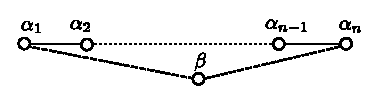
\includegraphics[scale=0.8]{305b.eps}}\\{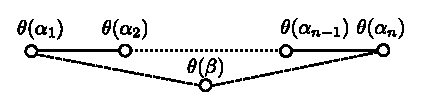
\includegraphics[scale=0.8]{305c.eps}}\end{tabular} & \begin{tabular}{c}
$\{\alpha_i , \theta (\alpha_i)\}$\\[0.5cm]
$2 i \neq n+1$ 
\end{tabular}\\\hline
\begin{tabular}{c}
$D_n, n$ odd\\[0.1cm]
$n > 3$
\end{tabular}  & \begin{tabular}{c}{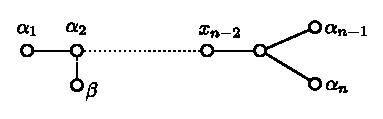
\includegraphics[scale=0.8]{305d.eps}}\end{tabular}  & $\{\alpha_{n-1}\}$ or $\{\alpha_n\}$\\\hline
\begin{tabular}{c}
$D_n \times D_n$\\[0.3cm]
$n$ odd \\[0.3cm]
$n > 3$
\end{tabular} & 
\begin{tabular}{c}
{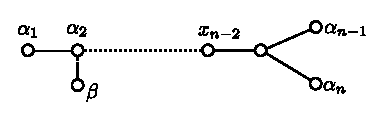
\includegraphics[scale=0.8]{305e.eps}}\\
{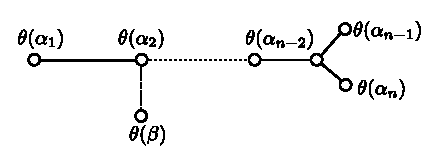
\includegraphics[scale=0.8]{305f.eps}}
\end{tabular} 
&
\begin{tabular}{c}
$\{\alpha_{n-1}, \theta (\alpha_{n-1})\}$\\[0.2cm]
or\\[0.2cm]
$\{\alpha_n, \theta(\alpha_n)\}$
\end{tabular}\\\hline
$E_6$
&
\begin{tabular}{c}
{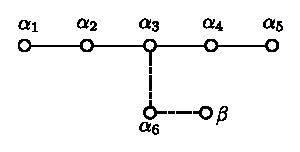
\includegraphics[scale=0.8]{305g.eps}}
\end{tabular}
&
\begin{tabular}{c}
$\alpha_1$ or $\alpha_2$\\[0.3cm]
or $\alpha_4$ or $\alpha_5$
\end{tabular}\\\hline
$\fprod{E_6}{E_6}{-}$ & 
\begin{tabular}{c}
{\includegraphics[scale=0.8]{305h.eps}}\\
{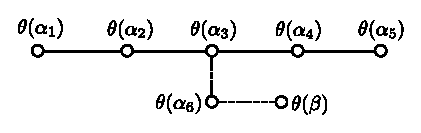
\includegraphics[scale=0.8]{305i.eps}}
\end{tabular}& 
\begin{tabular}{c}
$\{\alpha_1, \theta (\alpha_1)\}$ or\\[0.2cm]
$\{\alpha_2, \theta (\alpha_2)\}$ or \\[0.2cm]
$\{\alpha_4, \theta (\alpha_4)\}$ or \\[0.2cm]
$\{\alpha_5, \theta (\alpha_5)\}$
\end{tabular}\\\hline
\end{longtable}}\relax

\subsection{}\label{art9-subsec5.20}
~


{
\tabcolsep=3pt
\begin{longtable}{@{}|c|c|c|@{}}
\caption{($G$ absolutely simple)}\\
\hline
Type & 
\begin{tabular}{l}
Possible diagrams of $\bM_0$\\
as subdiagram  of $\Delta$ and \\
position of $\mu_0$, $\theta(\mu_0)$  
\end{tabular}& 
\begin{tabular}{l}
Possible diagrams of $\bM_1$\\
as subdiagram of $\Delta$ and \\
position of $\mu$, $\theta(\mu)$.
\end{tabular}\\
\hline
$A_n -$ I
& \begin{tabular}{c}
{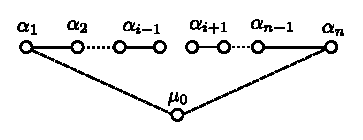
\includegraphics[scale=0.75]{306a.eps}}\\
$a < i <n/2$~ and ~$2i \neq n + 1$.
\end{tabular} &
\begin{tabular}{@{}l|l@{}}
\multicolumn{2}{l}{(a) $\bM_1 = \bM_0$; diagram as}\\
\multicolumn{2}{l}{in second column}\\\hline
(b)$^{\dagger}$ &  (c)\\
{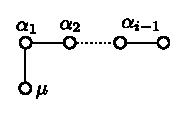
\includegraphics[scale=0.75]{306f.eps}} &
{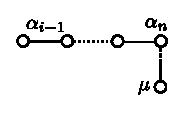
\includegraphics[scale=0.75]{306g.eps}}
\end{tabular} \\\hline
$A_n -$ II & \begin{tabular}{c}{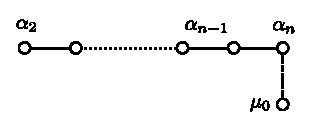
\includegraphics[scale=0.8]{306b.eps}}
\end{tabular} & 
\begin{tabular}{l}
$\bM_1 = \bM_0$; diagram as in\\
second column
\end{tabular}\\\hline
\begin{tabular}{c}
$D_n$\\
$n>3$
\end{tabular} & 
\begin{tabular}{c}
{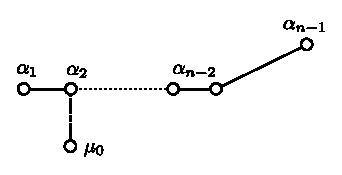
\includegraphics[scale=0.75]{306c.eps}}
\end{tabular}&
\begin{tabular}{l}
$\bM_1 = \bM_0$; diagram as in \\
second column
\end{tabular}\\\hline
$E_6-$ I & 
\begin{tabular}{c}
{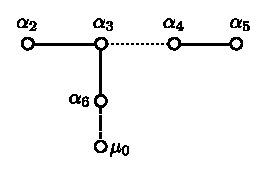
\includegraphics[scale=0.75]{306d.eps}}
\end{tabular}& 
\begin{tabular}{l}
$\bM_1 = \bM_0$; diagram as in \\
second column
\end{tabular}\\\hline
$E_6 -$ II & 
\begin{tabular}{c}
{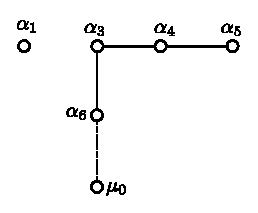
\includegraphics[scale=0.8]{306e.eps}}
\end{tabular} & 
\begin{tabular}{l}
$\bM_1 = \bM_0$; diagram is \\
same as in second column.\\
Here we use the classifi-\\
cation of real forms of $E_6$: \\
if the parabolic group\\
corresponding to $\alpha_2$ is \\
defined over $\bR$, real form \\
is split$^{\ddagger}$.
\end{tabular}\\\hline
\multicolumn{3}{l}{} \\[-0.2cm]
\multicolumn{3}{l}{($\dagger$) It is shown later that (b) cannot in fact occur.}\\
\multicolumn{3}{l}{($\ddagger$) See for example Tits \cite{art9-key1}.}
\end{longtable}}\relax


{
\tabcolsep=3pt
\begin{longtable}{@{}|c|c|@{}}
\caption{($G$ non-absolutely simple)}\\
\multicolumn{2}{l}{In this case $\bM_0 =\bM_1$ always.}\\\hline
Type & Diagram of $\bM_0 = \bM_1$ and position of $\mu$. \\\hline
$A_n \times A_n - I$ & 
\begin{tabular}{c}
{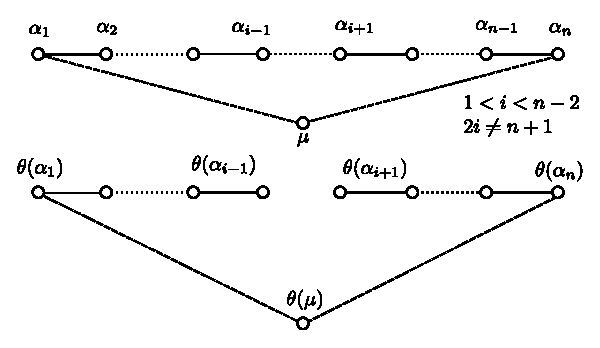
\includegraphics[scale=0.8]{307a.eps}}
\end{tabular}\\\hline
$A_n - $ II &
\begin{tabular}{c}
{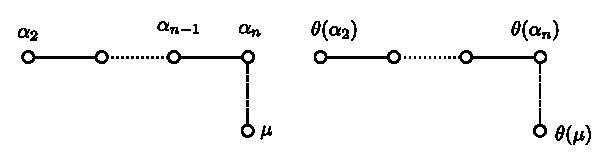
\includegraphics[scale=0.8]{307b.eps}}
\end{tabular}\\\hline
$D_n$ & 
\begin{tabular}{c}
{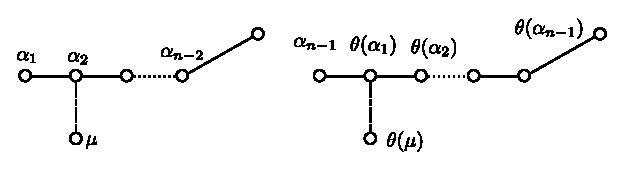
\includegraphics[scale=0.8]{307c.eps}}
\end{tabular}\\\hline
$E_6 - $ I &
\begin{tabular}{c}
{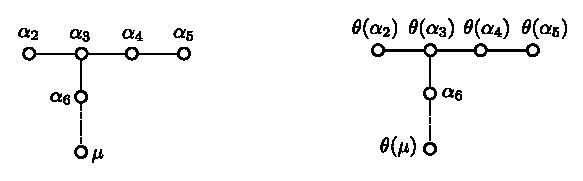
\includegraphics[scale=0.8]{307d.eps}}
\end{tabular}\\\hline
$E_6$ - II &
\begin{tabular}{c}
{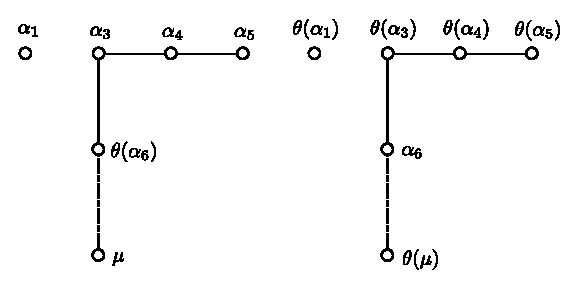
\includegraphics[scale=0.8]{307e.eps}}
\end{tabular}\\\hline
\end{longtable}
}\relax

\setcounter{subsection}{20}
\subsection{}\label{art9-subsec5.21}
From\pageoriginale Tables II and III, it is clear that if $\bM_0$ has two $\bR$-simple factors, then their absolute types are not the same. It follows that if $\bM_1 = \bM_0$ is not $\bR$-simple, then it breaks up also over $\bQ$ into exactly two factors. We will now treat two cases separately. Case A: $\bQ$-rank $\bM_1 > 1$; Case B: $\bQ$-rank $M_1 = 1$.

\subsection{}\label{art9-subsec5.22}
\textsc{Case A.} $\bQ$-rank $M_1 > 1$. If $\bM_1$ is $\bR$-simple, it is $\bQ$-simple. Now the following result is known (Raghunathan \cite{art9-key2}, \S \ref{art9-sec3}, Theorem 2).

Let $\Phi$ be an arithmetic subgroup of a $\bQ$-simple algebraic group $\bH$ of $\bQ$-rank $>1$. Then for any non-trivial irreducible representation $\rho$ of $\bH$, $H^1 (\Phi, \rho) =0$.

It is seen from Tables II and III \ref{art9-subsec5.20} that $M_1$ acts non-trivially on every simple factor of $\fK$. Hence in this case $H^1 (\Gamma_1, \fK) = 0$. Consider next the case when $M_1$ is not simple. In Tables II and III this corresponds to $A_n - I$ (a) and $E_6-$ II. In the case $A_n - I$, one sees that $\fK$ is (over $\bR$) a tensor product $\rho_1 \otimes \rho_2$ where $\rho_1$ and $\rho_2$ are faithful $\bR$-irreducible representations of the simple factors of $\bM_1$. Let $\bM_1 = \bM'_1 \times \bM''_1$. Then a subgroup $\Gamma_2$ of $\Gamma_1$ of finite index decomposes into a direct product of the form $\Gamma'_1 \times \Gamma''_2$, $\Gamma'_2 \subset \bM'_1$ and $\Gamma''_2 \subset \bM''_2$ According to Kunneth formula for cohomology we then find 
$$
H^1 (\Gamma_2, \rho) \simeq H^1 (\Gamma'_2 , \rho_1) \otimes H^0 (\Gamma''_2, \rho_2) \otimes H^0 (\Gamma'_2,\rho_1) \otimes H^1(\Gamma''_2, rho_2)
$$
and $H^0 (\Gamma'_2, \rho_1) = H^0 (\Gamma''_2, \rho_2) = 0$ since $\rho_1$ and $\rho_2$ are nontrivial. Finally, $H^1 (\Gamma_1, \rho) \to H^1 (\Gamma_2, \rho)$ is injective since $\Gamma_2$ has finite index in $\Gamma_1$. We are left with the case $E_6 - $ II now. In the discussion below in 5.23 - 5.24 we will prove the following. In the case of $E_6 - $ II, the (unique) simple component of type $A_4$ has $\bQ$-rank \textit{at least} 2. Once this claim is admitted, we observe that factor acts non-trivially on $\fK$ while the other factor of type $A_1$ acts trivially on $\fR$. We can appeal to the theorem quoted above (applied to the factor of type $A_4$) and the Kunneth formula to conclude that $H^1 (\Gamma_1, \fK) =0$. Thus in case $\bQ$-rank $\bM_1 \geqslant 2$, $\bN$ is $\Gamma$-rational.

\subsection{}\label{art9-subsec5.23}
We introduce some additional notation now; this notation will be used in the entire sequel. Let $\bU \subset \bM_1$ be a maximal unipotent $\bQ$-subgroup. Let $\bU = \sigma^{-1} (\bU_1)$. Evidently, then $U/U \cap \Gamma$ is compact. Moreover $U \cap \Gamma$ is a maximal unipotent subgroup of $\Gamma$: in fact if $\theta$ generates\pageoriginale with $U \cap \Gamma$ a unipotent group and $X \in \fg$ is the nilpotent element such that $\exp X = \theta$, then $X$ is orthogonal to $\ff$ w.r.t. $\langle , \rangle$ and hence belongs to $\fn$ so that $\exp X = \theta \in N$; it follows that $\sigma (\theta) \in \bU_1$ so that $\theta \in U \cap \Gamma$. Let $\bU^\ast$ be a maximal unipotent subgroup of $\bG$ containing $\bU$. Let $\gamma \in \Gamma$ be an element such that $\gamma U^\ast \gamma^{-1} \cap U^{\ast} = \{e\}$. For a subgroup $H$ of $\bG$, let $H^-= \gamma H \gamma^{-1}$. Then clearly $U^-/ U^- \cap \Gamma$ is compact. Since $N_0 / N_0 \cap \Gamma \to G/ \Gamma$  is proper, $N_0 \cap U^- \cap \Gamma$ is a lattice in $N_0 \cap U^-$. Let $U^-_1 = \sigma(N_0 \cap U^-)$. Then $\bU^-_1$ is defined over $\bQ$. Now from the structure of parabolic subgroups and our choice of $\gamma$ one deduces easily that $\dim \bU^-_1 =\dim \bU_1$. Thus $\bU^-_1$ is also a maximal unipotent subgroup of $\bM_1$. Let $\bP^-_1$ (\resp $\bP_1$) be the normaliser of $\bU_1$ (\resp $\bU^-_1$) in $\sigma (\bM_0)$. Then $\bP_1$ and $\bP^-_1$ are easily seen to be opposed to each other. Choosing $\bM$ so that it normalises $\bF$ and $\bF^-$, we can also choose $\bT$ (\cf \ref{art9-subsec5.15}) to normalise $\bU$ and $\bU^-$ and to have all roots is $\fu$ positive. We assume such a choice made; then the parabolic subgroup $P_1$ can be described as the maximal parabolic subgroup of $\bM_0$ associated to certain roots in the diagrams of $\bM_0$ and as indicated below:

\subsection{}\label{art9-subsec5.24}
We use the notation of Tables II and III.

{
\tabcolsep=3pt
\begin{longtable}{@{}|l|l|@{}}
\caption{}\\
\multicolumn{2}{l}{(A). $G$ absolutely simple.}\\\hline
\multicolumn{1}{|c|}{Type of $(\bG, \bM_0)$} & \multicolumn{1}{c|}{Roots defining the parabolic $P_1$}\\\hline
\qquad $A_n-$ I & \qquad \qquad $\alpha_{n+1-i}$\\
\qquad $A_n -$ II & \qquad \qquad $\alpha_n$\\
\qquad $D_n$ & \qquad \qquad $\alpha_{n-1}$\\
\qquad $E_6 -$ I & \qquad \qquad $\alpha_5$\\
\qquad $E_6 -$ II & \qquad \qquad $\alpha_4$\\\hline
\multicolumn{2}{l}{} \\[-0.2cm]
\multicolumn{2}{l}{(B) $G$ non-absolutely simple}\\\hline
Type of $G$ & Roots associated to $P_1$\\
\hline
\quad $A_2 \times A_n -$ I & \qquad $(\alpha_{n+1-i},\theta(\alpha_{n+1-i}))$\\
\quad $A_n \times A_n- $ II & \qquad $(\alpha_n, \theta(\alpha_n))$\\
\quad $D_n \times D_n$ & \qquad $(\alpha_{n-1}, \theta(\alpha_{n-1}))$\\
\quad $E_6 \times E_6 -$ I & \qquad $(\alpha_5 , \theta(\alpha_5))$\\
\quad $E_6 \times E_6 $ - II &  \qquad $(\alpha_4, \theta(\alpha_4))$\\\hline
\end{longtable}
}

Table IV\pageoriginale shows immediately--since $\bU_1 \subset \bM_1$--that the possibility (b) in $A_n - I$, Table II, is ruled out. Also, in the case of $E_6 -$ II, this shows that the $\bR$-simple component of type $A_4$ in $\bM_0$ does occur in $\bM_1$ as an isotropic factor. Moreover, the parabolic group $\bP_1$ in this case is non-symmetric. It follows that this component of $\bM_1$ (and hence $\bM_1$ itself) cannot have $\bQ$-rank 1 in this case. (This was what was claimed in \ref{art9-lem4.22}) Symmetry arguments show that $\bM_1$ can have $\bQ$-rank 1 only in the following cases:
\begin{tabular}{llll}
(1) & $A_{3r-1} -$ I, $i = r$. & (1$'$) & $A_{3r-1} \times A_{3r-1} - $ I, $i = r$. \\
(2) & $A_2 - $ II & (2$'$) & $A_2 \times A_2 -$ II \\
(3) & $E_6 - $ II & (3$'$) & $E_6 \times E_6 -$ II. 
\end{tabular}

\subsection{}\label{art9-subsec5.25}
We shall consider now the cases ($A_{3r-1} - $ I, $i=r$) and ($A_{3r-1} \times A_{3r-1}$, $i = r$) with $r \geqslant 2$. In the case ($A_{3r-1} -$ I, $i=r$) since the maximal parabolic subgroups corresponding to the roots $\alpha_r$  and $\alpha_{2r}$ are defined over $\bR$, the classification of $\bR$-simple groups of Type $A_n$ show that over $\bR$ both factors of $\bM_0$ are isotropic except when $r = 2$ and $\bG$ is not quasi-split over $\bR$ (see for instance Tits \cite{art9-key1}).

As already shown, in the non-absolutely simple case $A_n \times A_n - $ I, $n \geqslant 2$, $\bM_0$ has two factors both isotropic over $\bR$. Moreover, as remarked earlier again, these factors do not have isomorphic absolutely simple components. Thus $\bM_0 = \bM_1$ decomposes over $\bQ$ into two factors $\bM'_0 \times \bM''_0$ both of which are isotropic over $\bR$. The group $\Gamma_1$ decomposes---upto fintie index-into a product and since the representation on $\fK$ is a tensor product of non-trivial $\bR$-irreducible representations of the factors $\bM'_0$ and $\bM''_0$, the Kunneth formula can again be applied to establish that $H^1 (\Gamma_1, \fK) =0$.

\subsection{}\label{art9-subsec5.26}
The preceding discussion shows that except possibly in the case of $E_6 -$ II and $E_6 \times E_6 -$ II, if $\bM_1$ has $\bQ$-rank 1, $\bG$ has $\bR$-rank exactly 2. In all these cases we argue as follows: let $\alpha$ (\resp $(\alpha, \theta (\alpha))$) be the unique element (\resp pair) in $\Delta$ determining the parabolic subgroup $\bN$ in $\bG$. Let $\alpha$ (\resp ($\alpha$, $\theta(\alpha)$)) denote the unique element (\resp pair) equivalent to $\alpha$ (\resp $(\alpha, \theta(\alpha))$) under the non-trivial symmetry of $\Delta$. Let $\lambda$ (\resp $\lambda^\wedge$) denote the fundamental weight\pageoriginale associated to $\alpha$ (\resp $\hat{\alpha}$). Let $\omega_1$ be the element in the Weyl group of $\bM_0$ which changes the sign of all the roots of $\bM_0$. A simple computation then shown the following:
\begin{equation}
w_1 (\lambda - \mu) = \mu \text{ and } w_1\theta (\lambda - \mu) = \theta (\mu). 
\tag{($\ast$)}
\end{equation}
(In fact one has, $\omega_1 (\lambda) = \lambda$ while $w_1 (\mu) = \lambda - \mu$). Now let $\fT$ be the Lie algebra of $\fT$ and $H_\lambda$ (\resp $H_\mu$) the unique element in $\fT$ such that $\langle H, H_\lambda\rangle  = \lambda (H)$ (\resp $\langle H, H_\mu \rangle = \mu (H)$). Let $H^\ast_\lambda = (H_\lambda + \theta (H_\lambda))/2$ and $H^\ast_\mu = (H_\mu + \theta (H_\mu)/2)$; then $\ad H^\ast_\lambda$ and $\ad H^\ast_\mu$ are semisimple and their eigen-values are $\pm 1$ and 0. Further $\fF$ (\resp $\fF^-$) is the eigen-space of $\ad H^\ast_\lambda$ (\resp $\ad H^\ast_\mu$) corresponding to the eigen-value + 1 (\resp $-1$). It is also easy to verify the following: $\fu$ (\resp $\fu^-$) is the span of eigen-spaces of $\ad (H^\ast_\lambda + H^\ast_\mu)$ corresponding to the eigen-values 1 and 2 (\resp $-1$ and $-2$); moreover, the centre $\fC$(\resp $\fC^-$) of $\fu$(\resp $\fu^-$) is the eigen-space corresponding to the eigen-value 2 (\resp $-2$). Let $H = H^\ast_\lambda - H^\ast_\mu$. Let $\fB$ be the eigen-space of $H$ corresponding to the eigen-value 1. According to ($\ast$), this eigen-space is conjugate to the parabolic group \textit{opposed} to $\fF^-$ (w.r.t. $\bT$) (note that $\fF$ and $\fF^-$ are not opposed to each other). The corresponding subgroup $\bV$ of $\bG$. Moreover, it is easy to see that $\fo = \fn_0 \cap \ff^- + \fn^-_0 \cap \ff$. Since $(N^-_0 \cap F)/(N_0 \cap F \cap \Gamma)$ and $(N_0 \cap F^-)/(N_0 \cap F^- \cap \Gamma)$ are compact, $V/V \cap \Gamma$ is compact. It follows that if $\rho$ denotes the adjoint representation of $\bP$ on $\fB$ and $\bP_0 = \{x \in \bP \big| \det \rho (x) = \pm 1\}$ and $P_0 =\bP_0 \cap G$, then $P_0/P_0 \cap \Gamma \to G / \Gamma$ is proper. Also $\fB$ carries a $\bQ$-structure determined by a lattice $\sM$ in $\fB$ such that the map $P_0/ P_0 \cap \Gamma \to GL (\fo)/ GL (\sM)$ is proper. Now, by general position argument, we can find $\varphi\in \Gamma $ such that $\varphi \bP \varphi^{-1}$ is opposed to $\bF$ (as also to $\bF^-$). The arguments in \ref{art9-subsec5.4} with minor modifications now show that $\bN$ is $\Gamma$-rational.

This completes the proof of the main theorem.
 


\appendix

\begin{center}
{\textbf{\Large{Appendix I}}}\labeltext{I}{art9-app-I}
\end{center}

\renewcommand{\thesection}{A.\arabic{section}}

\section{}%% A.1 
Let $\bG$ be\pageoriginale a connected algebraic group defined, simple and of rank $\geqslant 2$ over $\bR$. Let $\bP$ be an $\bR$-parabolic subgroup of $\bG$ and $\bU$ the unipotent radical of $\bP$. Let $\fu$ be the Lie algebra of $\bU$ and $\sigma : \bP \to GL (\fu)$ the adjoint representation of $\bP$ on $\fu$. Let $\bM$ be a maximal reductive $\bR$-subgroup of $\bP$ and $\bM^\ast$ the product of the maximal $\bR$-split central torus $\bS$ in $\bM$ and all the $\bR$-isotropic $\bR$-simple components of $\bM$. Let $\bM^\ast_0$ be the identity component of 
$$
\bM^{\ast'}_0 = \{x \in \bM^\ast \big| \det \sigma (x) = \pm 1\},
$$
and $\bS_0$ the identity component of 
$$
\fS'_0 = \{x \in \fS \big| \det \sigma (x) = \pm 1\} = \bS \cap \bM^{\ast'}_0.
$$
With this notation we will prove the following two results. 

\section{}%%% A.2
\begin{alphlemma}\label{art9-lem-A}
Assume that $\bG$ has no absolutely simple component of type $\bG_2$. Then the centraliser of $\bM^\ast_0$ in $\fu$ is contained in the centre of $\fu$.
\end{alphlemma}

\section{}%%% A.3
\begin{alphlemma}\label{art9-lem-B}
Assume that the absolutely simple components of $\bG$ are all of the following types : $A_n$, $D_n$, $n$ odd $> 3$, or $E_6$. Let $\bP$ be non-maximal and `non-symmetric'--\ie $\bP \cap g \bU g^{-1} \neq \{e\}$ for any $g \in G$. Then $\bS_0$ acts non-trivially and as scalar automorphisms on the centre $\fC$ of $\fu$.
\end{alphlemma}

\section{}\label{art9-appsec-A4}%%% A.4
\begin{notation*}
Choose tori ${}_\bR \bT$ and $\bT$ such that $\bS \subset {}_\bR \bT \subset \bT \subset \bM$ and ${}_\bR \bT$ (\resp $\bT$) is maximal $\bR$-split (\resp maximal and defined over $\bT$) in $\bG$. Introduce compatible orderings on $X(\bT)$ (= group of characters on $\bT$) and $X ({}_\bT \bT)$ (= group of characters on ${}_\bR \bT$). Let $\Phi$ denote the roots of $G$ w.r.t. $\bT$. For $\alpha \in \Phi$, let $\fG (\alpha)$ denote the root space of $\alpha$ in the Lie algebra $\fG$ of $\bG$. Let $\fM$ denote the Lie subalgebra corresponding to $\bM$ and let $\Phi (\bM) = \{\alpha \in \Phi \big| \fG (\alpha) \subset \bM\}$. We assume the order on $X (\bT)$ so chosen that for $\alpha \in \Phi$, if $\fG (\alpha) \subset \fu$ (= Lie algebra of $\bU$), $\alpha > 0$. Let $\Delta$ denote the system of simple roots and $\Delta (M) = \Delta \cap \Phi (\bM)$. Let $\Delta' = \Delta - \Delta (\bM)$; then 
\begin{itemize}
\item[(i)] $\{\fG (a) \big| \alpha \in \Delta (\bM)\}$ generate $[\fM, \fM]$ as a Lie algebra ($\Delta (\bM)$ is a simple root system for $\fM$) and 

\item[(ii)] $\fu$ is\pageoriginale the linear span of
$$
\left\{\fG (a) \big| \alpha = \sum\limits_{\varphi \in \Delta} m(\varphi) . \varphi \text{ with } m (\varphi ) >0 \text{ for some } \varphi \in \Delta'  \right\}.
$$
\end{itemize}
Let $2 \rho $(\resp $2\rho(\bM)$) denote the sum of the positive roots of $\bG$ (\resp $\bM$). Then one sees from the definition of $\sigma$ that for $x \in \bT$, 
\begin{equation}
\det \sigma (x) = (2 \rho - 2 \rho (\bM)) \;(x).  \tag*{$(\ast)$}\label{art9-eqapp-*}
\end{equation} 
Let $\theta$ be the involution of $X (\bT)$ defined by complex conjugation; then $\theta(\Phi) = \Phi$. Further if $\alpha \in \Delta$ is non-trivial on ${}_\bR \bT$, there exists a unique element $\hat{\alpha} \in \Delta$ such that $\hat{\alpha}$ is non-trivial on ${}_\bR \bT$ and 
\begin{equation}
\theta (\alpha) = \hat{\alpha} + \sum\limits_{\varphi \in \Delta} m (\varphi) \varphi \tag*{$(\ast\ast)$}\label{art9-eqapp-**}
\end{equation}
with $m(\varphi) \neq 0$ only if $\varphi$ is trivial on ${}_\bR \bT$; if $\bG$ is \textit{not} absolutely simple $\theta(\alpha) = \hat{\alpha}$. Finally all the elements in $\Delta'$ are non-trivial on ${}_\bR \bT$ and for $\alpha \in \Delta'$, $\hat{\alpha} \in\Delta'$ (this is true since $\bP$ is defined over $\bR$). Finally we also note that since $\bM$ is defined over $\bR$,
\begin{equation}
\theta (\alpha) \in \Phi (\bM) \text{ for all } \alpha \in \Phi (M) ; \tag*{$(\ast\ast\ast)$}\label{art9-eqapp-***}
\end{equation}
in particular $\Phi(\bM)$ and $\theta (\Phi (\bM))$ are linear combinations of elements in $\Delta (\bM)$. After these preliminary common remarks, we will now first take up the proof of Lemma \ref{art9-lem-A}.
\end{notation*}

\section{Proof of Lemma \ref{art9-lem-A}}%%% A5
Let $\fC$ be the centre all $\fu$. Suppose now that $E \not\in \fC$. Since $\bM^\ast_0$ is normal in $\bM$, $E$ is $\bM$-stable. On the other hand $\fC$ is evidently $\bM$-stable. Let $E'$ be an $\bM$-stable supplement to $E \cap \fC$ in $E$ ($E'$ is in fact unique since $\bT \subset \bM$ and $\fu$ is a sum of mutually inequivalent simple $\bT$-modules). Let $\beta'$ be the highest root in $\Phi$ such that $\fG (\beta') \subset E'$. We then have (for the natural scalar product on $X(T)$),
\begin{equation*}
\left.
\begin{aligned}
& \langle \varphi, \beta' \rangle  \geqslant 0 \text{ for all  } \varphi \in \Delta (\bM) \text{ and }\\
& \langle \varphi, \beta' \rangle = 0 \text{ for } \varphi \in \Delta (\bM^\ast) = \{\alpha \in \Delta \big| \fG (\alpha) \subset \fM^\ast_0\} 
\end{aligned}
\right\}
\tag{I} 
\end{equation*}
(here $\fM^\ast_0$ = Lie algebra of $M^\ast_0$). Further, since $\beta'(x) =1$ for all $x \in_\bR \bT^0 = \{y \in \bT \big| \det \sigma(y) =1\} \; (\subset \bM^\ast_0)$ we have necessarily
$$
\beta \big|_{\bR} \bT = p (2\rho -2 \rho (\bM)) \big|_{\bR} \bT \text{ with } p > 0.
$$

If $\lambda$\pageoriginale is any character on $\bT$, $\lambda + \theta (\lambda)$ is defined over $\bR$ so that if $\mu$ and $v$ are characters on $\bT$ which coincide on ${}_\bR \bT$, we have $v+ \theta(v) = \mu + \theta(\mu)$. Also $\theta(\lambda) = \lambda$ if and only if $\lambda$ is defined over $\bR$. These considerations show that 
$$
\beta' + \theta (\beta') = q (2\rho - 2 \rho (M)), \; q > 0.
$$
Now as is well known we have 
\begin{equation*}
\left. 
\begin{aligned}
& 2 \langle \rho, \alpha \rangle  = \langle \alpha, \alpha \rangle  \hspace{1cm} \text{ for } \alpha \in \Delta \text{ and }\\
&  2 \langle \rho (\bM), \alpha \rangle  = \langle \alpha, \alpha \rangle  \quad \text{ for } \alpha \in \Delta (\bM).
\end{aligned}
\right\}
\tag{II}
\end{equation*}
It follows that
\begin{align*}
\langle \beta' + \theta (\beta'), \alpha \rangle & = 0 \text{ for  } \alpha \in \Delta (\bM)\\
& = r \langle \alpha, \alpha \rangle \text{ for } \alpha \in \Delta'
\end{align*}
for a suitable \textit{ positive } number $r$. Suppose now that $\langle \beta, \alpha \rangle < 0$ for some $\alpha \in \Delta'$; then we have 
$$
2 \langle \beta', \alpha \rangle  = - k \langle \alpha, \alpha \rangle 
$$
where $k = \langle \beta', \beta' \rangle / \langle \alpha, \alpha \rangle $; since $\langle \theta (\beta'), \alpha \rangle / \langle \alpha, \alpha  \rangle \leqslant k \langle \alpha, \alpha \rangle $, in this case, we are led to a contradiction. Thus we necessarily have (combining with ($\ast$))
$$
2 \langle \beta', \alpha \rangle  \geqslant 0 \text{ for all } \alpha \in \Delta.
$$
Suppose $\alpha \in \Delta'$ is a root such that $\beta' + \alpha$  is again a root, then we have
$$
\langle \beta' + \alpha, \beta' + \alpha \rangle = \langle \beta', \beta' \rangle + \langle  \alpha, \alpha \rangle + 2 \langle \beta', \alpha \rangle .
$$
Since $\beta'$ is not the highest root, we see that such a root a exists; it follows that there are \textit{necessarily two root lengths}. Moreover, if $\langle \beta',\alpha \rangle \neq 0$, $\beta' + \alpha$ is atleast thrice as long as the shorter of the roots $(\alpha, \beta')$. Thus since $\bG$ has no components of type $G_2$ we are led to the following conclusion: (absolutely) simple components of $\bG$ are of type $B_n$, $C_n$ or $F_4$ and 
\begin{equation*}
\left. 
\begin{aligned}
\langle \beta' ,\alpha \rangle & \geqslant 0 \text{ for all } \alpha \in \Delta \\
& = 0 \text{ for } \alpha \in \Delta (\bM^\ast) \cup \Delta'. 
\end{aligned}
\right\}
\tag{III}\label{art9-app-III}
\end{equation*}
Now if $\beta$ denotes the highest root, $\beta = \beta' + \sum\limits_{\varphi \in \Delta} m (\varphi). \varphi$ with $m(\varphi) \geqslant 0$ so that from \ref{art9-app-III} we deduce that $\langle \beta, \beta \rangle > \langle \beta', \beta' \rangle$. Thus $\beta'$ is the unique short\pageoriginale root which is a dominant weight. Now since $\bM^\ast_0$ contains all the isotropic simple factors of $\bM$, one sees that the roots $\alpha \in \Delta$ which are non-trivial on ${}_\bR \bT$ are necessarily contained in $(\Delta (\bM^\ast) \cup \Delta')$. \textit{ In particular if $\langle \beta', \alpha \rangle > 0$ for $\alpha \in \Delta, \alpha$ is trivial on ${}_\bT \bT$}. We now list below the possible Tits diagrams for $\bG$ showing also to which simple roots $\beta$ and $\beta'$ are lined. Roots in $\Delta$ which are non-trivial on ${}_\bR \bT$ are indicated by drawing a circle around them. The arrows point towards the short root.

\medskip
\noindent
\textsc{Case I.} $G$ \textit{absolutely simple} (note that $R$-rank $G \geqslant 2$). $r = \bR-rank G$. 
{
\tabcolsep=1.5pt
\setcounter{table}{0}
\begin{longtable}{@{}|c|cl|@{}}
\hline
Type & \multicolumn{2}{c|}{Diagram}\\\hline
$B_{n,r}$ & 
\begin{tabular}{c}
{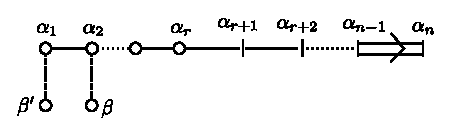
\includegraphics[scale=0.73]{315a.eps}}
\end{tabular} & 
\begin{tabular}{l}
$\{\alpha_i \big| 1 \leqslant i \leqslant r \}$ are\\
non-trivial on ${}_\bR \bT$
\end{tabular}\\
\begin{tabular}{c}
$C^{(1)}_{n,r}$\\
$(n = r)$
\end{tabular} & 
\begin{tabular}{c}
{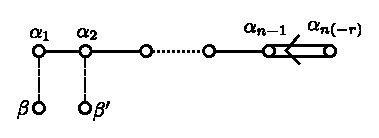
\includegraphics[scale=0.73]{315b.eps}}
\end{tabular} &
\begin{tabular}{l}
$\bT = {}_\bR \bT$; all roots are \\
non-trivial on ${}_\bR \bT$
\end{tabular}\\
\begin{tabular}{c}
$C^{(2)}_{n,r}$\\
$(n>2r)$
\end{tabular} & 
\begin{tabular}{c}
{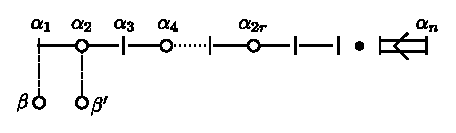
\includegraphics[scale=0.73]{315c.eps}}
\end{tabular} &
\begin{tabular}{l}
$\{\alpha_{2i} \big| 1 \leqslant i \leqslant r\}$ are \\
non-trivial on ${}_\bR \bT$
\end{tabular}\\
\begin{tabular}{c}
$C^2_{n,r}$\\
$(n=2r)$
\end{tabular}& 
\begin{tabular}{c}
{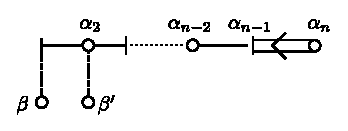
\includegraphics[scale=0.73]{315d.eps}}
\end{tabular}&
\begin{tabular}{l}
$\{\alpha_{2i} \big| 1 \leqslant i \leqslant r\}$ are\\
non-trivial on ${}_\bR \bT$.
\end{tabular}\\
\begin{tabular}{c}
$F^0_{44}$\\
$(n=r=4)$
\end{tabular} & 
\begin{tabular}{c}
{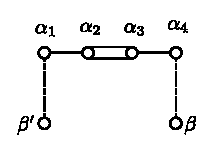
\includegraphics[scale=0.73]{315e.eps}}
\end{tabular} & 
\begin{tabular}{l}
${}_\bR \bT = \bT$; all roots are\\
non-trivial on ${}_\br \bT$.
\end{tabular}\\\hline
\end{longtable}}\relax

\medskip
\noindent
\textsc{Case II.} $\bG$\pageoriginale \textit{non-absolutely simple}. In this situation every root of $\bG$ is necessarily non-trivial on ${}_\bR \bT$.

The table on p. 315 shows that the short dominant root has always a non-trivial scalar product with a simple root which is non-trivial on ${}_\bR \bT$, leading to a contradiction.
 
\section{Proof of Lemma \ref{art9-lem-B}}%%% A.6
The fact that $\bP$ is non symmetric leads us in the first place immediately to the conclusion that the (absolutely) simple components of $\bG$ are of one of the following types: $A_n$, $D_n$ ($n$ odd) or $E_6$: these are the groups in which the Weyl group element that takes all simple roots into negative roots, is different form $x \longmapsto -x$ (on the character group of the maximal torus); this automorphism is in fact of the form $\alpha \longmapsto - \tau (\alpha)$, where $\tau$ is the unique \textit{non-trivial symmetry} of the Dynkin diagram of each simple factor. The subset $\Delta'$ corresponding to the parabolic group, one now observes, must necessarily be \textit{not} stable under $\tau$. Since $\bP$ is defined over $\bR$, $\alpha$ is non-trivial on ${}_\bR\bT$ for all $\alpha \in \Delta'$ and for $\alpha \in \Delta'$, $\hat{\alpha} \in \Delta'$. Finally since $\bP$ is non-maximal, there exist a pair $\alpha$, $\alpha_2 \in \Delta'$ such that $\alpha_1 \neq \hat{\alpha}_2$. The torus $\bS$ is precisely the identity component of the intersection ${}_\bR \bT \bigcap\limits_{\alpha \in \Delta - \Delta'} \ker \alpha$. Now it is easy from the description of $\fu$ as a sum of root spaces of $\fG$ that the centre $\fC$ of $\fu$ is in fact an $\bR$-irreducible $\bM$-module. Since $\bS$ is $\bR$-split and \textit{central} in $\bM$, $\bS$ acts as scalars on $\fC$ (Schur's lemma). Finally if $\beta$ is a highest root of $\fG$, $\fG (\beta) \subset \fu$. In view of our remarks in \ref{art9-appsec-A4} (in particular \ref{art9-eqapp-*} and \ref{art9-eqapp-***}) Lemma \ref{art9-lem-B} reduces to the following assertion:

The set of roots $(\Delta - \Delta' ) \cup \{\beta, 2 \rho - 2 \rho (\bM)\}$ restricted to ${}_\bR \bT$ are linearly independent. Equivalently,
$$
\Delta - \Delta' \cup \{\beta + \theta (\beta), 2\rho\}
$$
are linearly independent in $X(\bT)$ (note that for $\alpha \in \Delta - \Delta' = \Delta (\bM)$, $\theta(\alpha)$ is again a linear combination of elements in $\Delta (M)$). From \ref{art9-eqapp-**} of \ref{art9-appsec-A4}, we see immediately that if 
$$
\beta = \sum\limits_{\varphi \in \Delta} p (\varphi) . \varphi
$$\pageoriginale 
and 
$$
\theta (\beta) = \sum\limits_{\varphi \in \Delta} \hat{p} (\varphi) \varphi,
$$
then $\hat{p}(\varphi) = p (\varphi)$ for all $\varphi$ which are non-trivial on ${}_\bR\bT$, in particular for $\varphi \in \Delta'$. Now, let
$$
\beta + \theta (\beta) = \sum\limits_{\varphi \in \Delta} r (\varphi)\cdot \varphi
$$
and 
$$
2 \rho = \sum\limits_{\varphi \in \Delta} q (\varphi) \cdot \varphi.
$$
We have to show then that there exist $\varphi_1$, $\varphi_2 \in \Delta'$ such that $r(\varphi_1)/ r (\varphi_2) \neq q (\varphi_1)/ q(\varphi_2)$. Let $\Delta_0$ be the set of elements of $\Delta$ which are trivial on ${}_\bR\bT$. Let $\kappa$ be the Weyl group element of the corresponding root system $\Phi_0$ (associated to $\Delta_0$) which takes all of $\Delta_0$ into negative roots. For $\alpha \in \Delta_0$, let $\hat{\alpha} = -\kappa (\alpha)$. Then $\longmapsto \hat{\alpha}$ is an automorphism of the diagram of $\Delta$; this automorphism of $\Delta$ cannot be the same as $\tau$  since $\Delta'$ is stable under it. It follows that in the absolutely simple case $\alpha = \hat{\alpha}$ for $\alpha \in \Delta$; in the non-absolutely simple case $\Delta$ breaks into two components and $\theta$ exchanges the two. One sees immediately from this that for all $\varphi \in \Delta'$, we have $p(\varphi) = \hat{p}(\varphi)$. The problem reduces once again to show that there exist $\varphi_1, \varphi_2 \in \Delta'$ such that $p(\varphi_1) / p (\varphi_2)$ is not equal to $q(\varphi_1)/q(\varphi_2)$. This can be seen immediately from the following table. (The first three are absolutely simple and the last three are not).
{
\tabcolsep=1.5pt
\fontsize{9}{11}\selectfont
\setcounter{table}{0}
\begin{longtable}{@{}|c|c|l|l|@{}}
\hline
Type & Diagram of $\bG$ & \;\; $p_i = p (\alpha_i)$, $p'_i = p (\beta_i)$ & \; $q_i = q (\alpha_i)$, $q'_i = q(\beta_i)$\\\hline
$A_n$ & 
\begin{tabular}{c}
{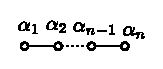
\includegraphics[scale=0.8]{318a.eps}}
\end{tabular} & \; $p_i = 1$ & $q_i = i (n-i+1)$\\\hline
\begin{tabular}{c}
$D_n$\\
$n$ odd \\
$n > 3$
\end{tabular} & 
\begin{tabular}{c}
{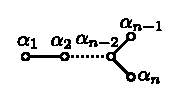
\includegraphics[scale=0.8]{318b.eps}}
\end{tabular} & 
\begin{tabular}{l}
$p_i = 2$ for $1 < i < n -1$ \\
\quad~ $= 1 $ for  $i = 1$, $n - 1$\\
\hspace{2cm} or $n$
\end{tabular} & 
\begin{tabular}{l}
$q_i = i (2n - i - 1)$\\
\qquad $l \leqslant i < n - 1$\\
$q_{n-1} = q_n = n (n -1) / 2$
\end{tabular}\\\hline
$E_6$ & 
\begin{tabular}{c}
{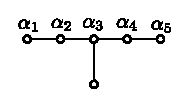
\includegraphics[scale=0.8]{318c.eps}}
\end{tabular}&
\begin{tabular}{l}
$p_1 = p_5 = 1 $, $p_2 = p_4 = $\\
$ p_6 = 2$, $p_3 = 3$
\end{tabular} & 
\begin{tabular}{l}
$q_1 = q_5 = 16$,\\
 $q_2 = q_4 = 15$\\
$q_3 = 21$, $q_6 =11$
\end{tabular}\\\hline
$A_n$ &
\begin{tabular}{c}
{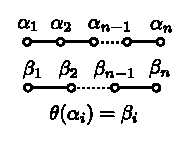
\includegraphics[scale=0.8]{318e.eps}}
\end{tabular} & 
$p_i = p'_i =1$ &
$q_i = q_i = i (n-i+1)$\\\hline
\begin{tabular}{c}
$D_n$ \\
$n$ odd\\
$n>3$
\end{tabular} & 
\begin{tabular}{c}
{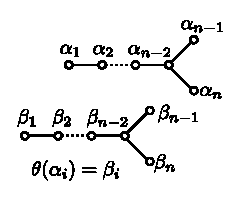
\includegraphics[scale=0.8]{318f.eps}}
\end{tabular} & 
\begin{tabular}{l}
$p_i = p'_i = 2$ for $1< i < n -1$\\
\quad $ = 1 $ for $i = 1$, $n -1$\\
\qquad \quad or $n$
\end{tabular} & 
\begin{tabular}{l}
$q_i = q'_i = i (2n - i -1)$\\
$q_{n-1} = q'_{n-1} = q_n =$ \\
$q'_n = n (n-1) /2$
\end{tabular} \\\hline
$E_6$ & 
\begin{tabular}{c}
{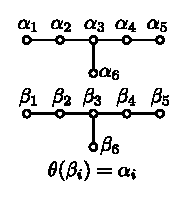
\includegraphics[scale=0.8]{318g.eps}}
\end{tabular}&
\begin{tabular}{l}
$p_1 = p'_1 = p_5 = p'_5 = 1$,\\
$p_2 = p'_2 = p_4 = p'_4 = 2$\\
$p_6 = p'_6 = 2$, $p_3 = p'_3 = 3$
\end{tabular} & 
\begin{tabular}{l}
$q_1 = q'_1 = q_5 = q'_5 = 16$,\\
$q_2 = q'_2 = q_4 = q'_4 = 15$\\
$q_3 = q'_3 = 21$, $q_6 = q'_6 = 11$
\end{tabular}\\\hline
\end{longtable}}\relax

\begin{center}
{\textbf{\Large{Appendix II}}}\labeltext{II}{art9-app-II}
\end{center}

\section{}%% A.7 
Let $A$ be\pageoriginale a ring and $B$ the centre of $A$. Let $M$ and $N$ be $A$-modules. Then a homothesy by an element $b \in B$ induces a $A$-linear map of $M$ in $M$. Consequently it induces a map
$$
\bar{b} : \Ext^p_A (M,N) \longrightarrow \Ext^p_A (M,N).
$$
It is a simple consequence of the definition of the groups $\Ext$ that this defines a structure of a $B$-module on $\Ext^p_A (M,N)$ and that this structure is the same as that obtained by treating an element $b \in B$ as the $A$-linear homothesy of $N$. An immediate result of this observation is the following:

\setcounter{appenprop}{7}
\begin{appenprop}\label{art9-appenpropA8}
Suppose $b \in B$ is such that corresponding homothesy of $M$ is trivial while that of $N$ is an automorphism of $N$; then $\Ext^p_A (M,N) = 0$ for $p \geqslant 0$.
\end{appenprop}

One has only to remark that $\bar{b}$ is both the zero map and an automorphism.

\begin{appencoro}\label{art9-appencoroA9}
Let $k$ be a field and $\pi$ (\resp $\fg$) a group (\resp a $k$-Lie algebra). Let $\rho$ be an `irreducible' representation of $\pi$ (\resp $\fg$) on a $k$-vector space $M$. Suppose there is a central element $x$ (\resp $X$) in $\pi$ (\resp $\fg$) such that $\rho (x) \neq$ identity (\resp $\rho(X) \neq 0 $). Then $H^p(\pi, \rho) =0$ (\resp $H^p (\fg, \rho) =0$) for all $p \geqslant 0$. 
\end{appencoro}

By definition $H^p(\Gamma, \rho) \simeq \Ext^p_{k(\pi)} (k, M) (\resp H^p(\fg, \rho) \simeq \Ext^p_{k(g)} (k, M))$ where $k(\pi)$ (\resp $k(\fg)$) is the group-algebra (\resp the enveloping algebra) of $\pi$ (\resp $\fg$), and $M$ is considered a $k(\pi)^-$ (\resp $k(\fg)^-$) module through the trivial action of $\pi$ (\resp $\fg$) on $k$. The element $b = x -1$ (\resp $=X$) is then a central element of $A = k(\pi)$ (\resp $= k (\fg)$) and the corollary follows directly from the proposition and Schur's lemma (note that $\rho$ is \textit{irreducible}).

\begin{appencoro}\label{art9-appencoroA10}
Let $\pi$ (\resp $\fg$) be an `abelian' group (\resp Lie algebra) and $\rho$ `any nontrivial' irreducible representation of $\pi$ (\resp $\fg$); then $H^p(\pi,\rho) =0$ (\resp $H^p (\fg, \rho) =0$) for all $p \geqslant 0$.
\end{appencoro}

This follows from Corollary 1 choosing for $x$ (\resp $X$) any element of $\pi$ (\resp $\fg$) such that $\rho (x) \neq 1$ (\resp $\rho(X) \neq 0$).

\begin{thebibliography}{99}
\bibitem{} \textsc{L. Auslander : [1]} Bieberbach's\pageoriginale theorem on space groups and discrete uniform subgroups, \textit{Ann. of Math.} 71 (1960), 579-590 II, \textit{Amer. J. Math.,} 86 (1961), 276-280.

\bibitem{} \textsc{A. Borel : [1]} Density properties of certain subgroups of semisimple groups, \textit{Ann. of Math.,} 72 (1960), 179-188.

\bibitem{} [2] Sousgroupes discrets de groupes semisimple, \textit{Seminaire Bourbaki} (1968-69), \textit{Expose} 358.

\bibitem{} [3] \textit{Linear algebraic groups,} Benjamin, New York, (1969).

\bibitem{} \textsc{A. Borel,} and \textsc{J. Tits:} [1] Groupes reductifs, \textit{Publ. Mathematiques, I.H.E.S.,} 27 (1965), 55-150.

\bibitem{} \'El\'ements unipotents et sous-groupes paraboliques de groups r\'eductifs. I., \textit{Inv. Math.,} 12 (1971), 95-104.

\bibitem{} \textsc{H. Garland} and \textsc{M. S. Raghunathan : [1]} Fundamental domains for lattices in ($R$-) rank 1 semisimple Lie groups, \textit{Ann. of Math.,} 92 (1970), 279-326.

\bibitem{} \textsc{D. A. Kazdan} and \textsc{G. A. Margolis :} [1] A proof of Selberg's, hypothesis, \textit{Math. Sbornik (N. S.)}, 75 (117)  (1968), 162-168 (Russian).

\bibitem{} \textsc{A. I. Mal'cev :} [1] On a class of homogeneous spaces, \textit{Amer. Math. Soc. Transl. No.} 39 (1951).

\bibitem{} \textsc{G. A. Margolis :} [1] On arithmeticity of discrete groups, \textit{Soviet. Math. Dokl., } 10 (1969), 900-902 (Russian).

\bibitem{} [2] On the action of unipotent groups in the space of lattices, \textit{Math. Sb,} 86 (1969), 552 (Russian).

\bibitem{} \textsc{G. D. Mostow : [1]} On maximal subgroups of real Lie groups. \textit{Ann. of Math., } 74 (1961), 503-517.

\bibitem{} \textsc{I. I. Pjatets$\check{\textsc{k}}\check{\textsc{i}}$-Shapiro} : [1] Discrete subgroups of Lie groups. \textit{Trudy Moskov. Mat. Obsc.,} 18 (1968) , 3-18.

\bibitem{} \textsc{M. S. Raghunathan : } [1] \textit{Discrete subgroups of Lie groups,} Springer-Verlag, New York (1972).

\bibitem{} [2] Cohomology of arithmetic subgroups of algebraic groups, I., \textit{Ann. of Math.} 86 (1967), 409-424.

\bibitem{} [3] A note on\pageoriginale quotients of real algebraic groups by arithmetic subgroups, \textit{Inv. Math.}

\bibitem{} [4] Lattices in semisimple Lie groups, \textit{Actes du Congr\`es International des math\'ematiciens} (Nice 1970), 2, 337-341, Gautier-Villars, Paris (1971).

\bibitem{} \textsc{M. Rosenlicht: } [1] Some rationality questions on algebraic groups, \textit{Ann. di. Math.,} 43 (1957),  25-50.

\bibitem{} [2] On quotient varieties and affine embedding of certain homogeneous spaces, \textit{Trans. Amer. Math. Soc.,} 101 (1961), 211-233.

\bibitem{} \textsc{J. Tits : } [1] Classification of semisimple algebraic groups, algebraic groups and discontinuous groups, \textit{A. M. S., Proceedings of Symposia in Pure Mathematics,} IX.

\bibitem{} \textsc{H. C. Wang :} [1] On the deformation of lattices in a Lie group, \textit{Amer. J. Math., 91 (1967), 921-937}.

\bibitem{} \textsc{H. Zassenhaus : } [1] Beweis eines Satzes uber diskrete Gruppen, \textit{Abh. Math. Sem. Hansisch. Univ.,} 12 (1938), 289-312.
\end{thebibliography}
